\chapter{泌尿系统疾病}

\chapterabstract{本章重点介绍肾小球疾病和肾盂肾炎;简单介绍肾细胞癌和膀胱乳头状移形细胞癌。要求掌握各种原发性肾小球肾炎的基本病变及临床病理联系,急、慢性肾盂肾炎的病理变化。熟悉肾细胞癌和膀胱移行细胞癌的组织学类型及生物学特性,各型原发性肾小球肾炎的病因、发病机制、分类。了解肾盂肾炎的病因与发生机制。}

泌尿系统由肾、输尿管、膀胱和尿道组成。其生理功能是排泄代谢废物及毒物,以维持机体内水、盐代谢,渗透压和酸碱平衡。肾脏是泌尿系统中最重要的脏器,以肾单位(nephron)为基本的结构和功能单位,由肾小球(glomerulus)和与之相连的肾小管(renal
tubule)及间质构成。肾小球是由入球小动脉和出球小动脉、肾球囊和伸入囊内的丛状的毛细血管襻组成。毛细血管襻是肾小球的基本结构,内衬内皮细胞,外为基膜和脏层上皮覆盖,并由系膜(mesangium)支持固定。肾小球滤过膜(filter
membrane)由内皮细胞(endothelial cell)、基膜(basement
membrane,BM)和脏层上皮细胞(visceral epithelial
cell)共同构成,其超滤屏障是尿液形成时所必需。肾球囊又称鲍曼囊(Bowman's
capsule),是肾小管盲端凹陷形成的杯状双层囊,分别由脏层上皮和壁层上皮构成,两层间的腔为肾小囊腔。脏层上皮有许多突起突向囊腔称为足突(foot
process),所以脏层上皮又被称为足细胞(foot cell or
podocyte)。系膜由系膜细胞(mesangial
cell)和基膜样的系膜基质(mesangial matrix)构成。

肾脏的主要功能是排泄代谢产物,调节水、电解质和酸碱平衡。肾脏还具有内分泌功能,分泌肾素(renin)、促红细胞生成素(erythropoietin,EPO)、前列腺素(prostaglandin,PG)和1,25-二羟胆骨化醇(1,25-dihydroxy
cholecalciferol)等。肾脏具有很强的代偿功能,但超过了其代偿能力,就可以发生各种肾脏疾病,严重时可发展成肾衰竭(kidney
failure)。

泌尿系统疾病中以累及肾脏的疾病对人体造成的危害性最为严重,而且是引起慢性肾衰竭的主要原因。泌尿系统的疾病很多,根据病因和病变发生的部位可分为以下几类:①以肾小球损害为主的疾病,如原发性肾小球肾炎;②以肾小管损害为主的疾病,如急性肾小管坏死;③血管源性疾病,如高血压病的肾细动脉硬化和动脉粥样硬化性肾硬化;④以间质病变为主的疾病,如急、慢性肾盂肾炎、肾结核;⑤泌尿道梗阻,如肾和尿路的结石、肾盂积水等;⑥先天性发育畸形,如多囊肾;⑦肿瘤,如肾细胞癌、肾母细胞瘤等。

\section{肾小球疾病}

肾小球疾病(glomerular
diseases),又称肾小球肾炎(glomerulonephritis,GN),是以肾小球损伤和改变为主的一组疾病。肾小球疾病可分为原发性肾小球肾炎、继发性肾小球疾病和遗传性肾炎(hereditary
nephritis)。原发性肾小球肾炎,肾是唯一或主要受累的脏器;而在继发性肾小球疾病时,肾的损害往往是全身性疾病损害的一部分。例如系统性红斑狼疮;血管病变如高血压和结节性多动脉炎;代谢性疾病如糖尿病;遗传性肾炎则显示有遗传性家族性疾病,例如Alport综合征(由于编码IV型胶原cx链的基因突变导致肾小球基膜变薄,出现血尿或蛋白尿等症状)、Fabry's病等。本章主要讨论原发性肾小球肾炎。

\subsection{肾小球肾炎的发病机制}

有两种基本的肾小球损伤的机制:免疫机制和非免疫机制。大部分原发性肾小球肾炎和许多继发性肾小球疾病是由免疫机制引起。

\subsubsection{免疫机制}

与肾小球肾炎有关的抗原分为内源性和外源性两大类。内源性抗原包括肾小球性抗原[肾小球基膜(glomerular
basement
membrane,GBM)抗原、足细胞、内皮细胞和系膜细胞的细胞膜抗原等]和非肾小球性抗原(DNA、核抗原、免疫球蛋白、肿瘤抗原和甲状腺球蛋白等);外源性抗原包括细菌、病毒、寄生虫、真菌和螺旋体等生物性病原体的成分,以及药物、外源性凝集素和异种血清等。

在肾小球内的抗原抗体复合物的沉积是肾小球损伤的主要机制,复合物可在肾小球原位形成或在循环中形成。少数可为细胞免疫机制。

\paragraph{原位免疫复合物性肾炎}
抗体能与肾小球原位抗原成分直接发生反应引起肾小球病变,这些原位抗原可能来自肾小球本身的固有抗原或经血液循环植入肾小球的植入抗原,多为不溶性的。相关的类型有:

(1)抗肾小球基膜抗体引起的肾炎:这是由抗肾小球基膜抗体与肾小球本身的抗原(肾小球基膜抗原)成分反应引起的自身免疫性疾病(图\ref{fig10-1})。

\begin{figure}[!htbp]
 \centering
 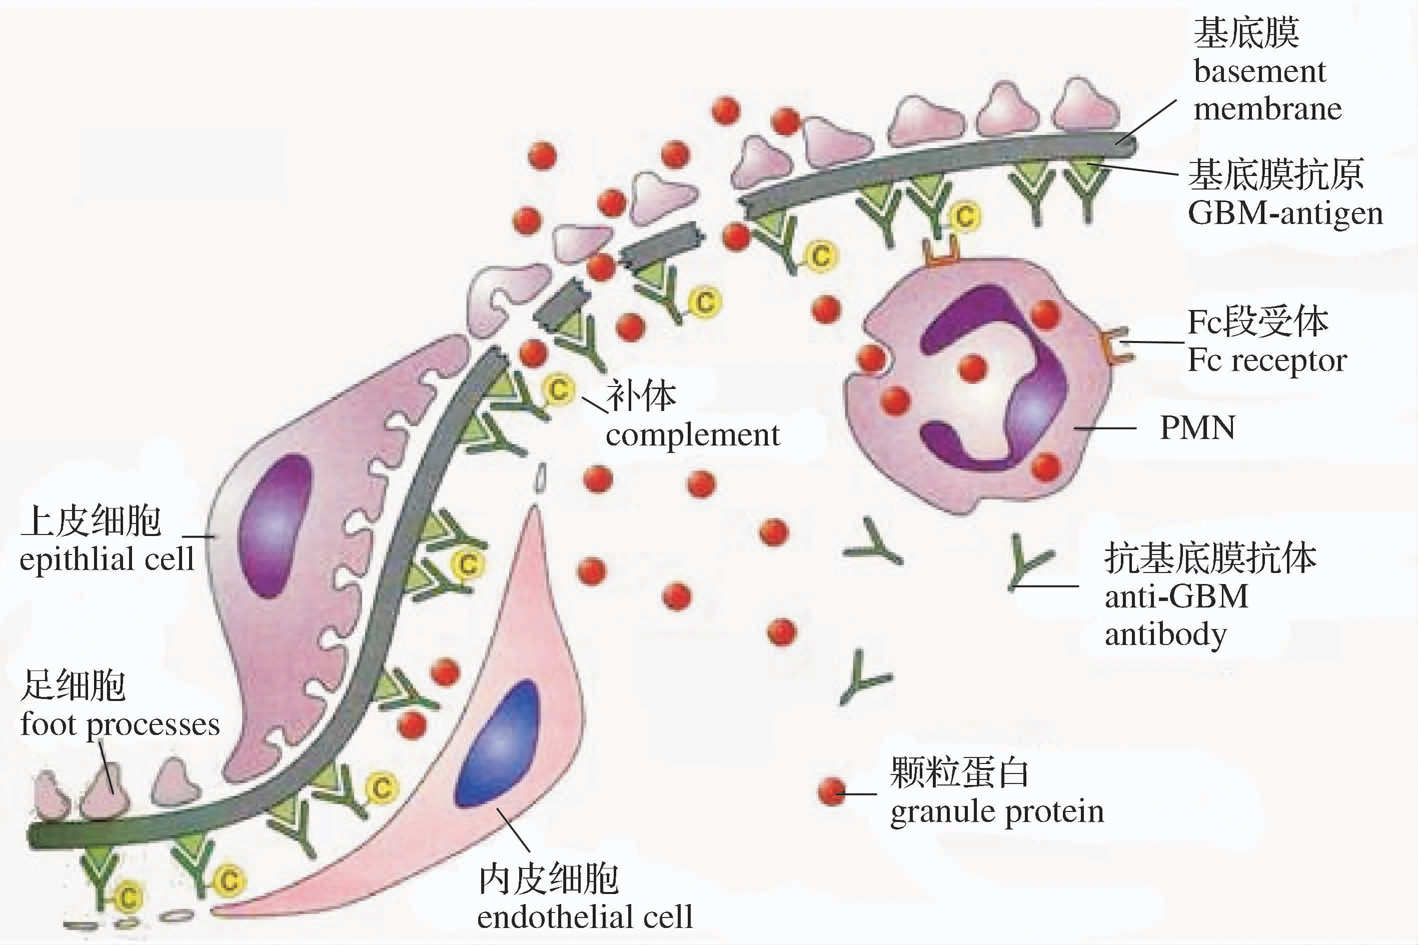
\includegraphics{./images/Image00147.jpg}
 \captionsetup{justification=centering}
 \caption{原位免疫复合物性肾炎的模式图}
 \label{fig10-1}
  \end{figure} 

显示抗肾小球基膜抗体引起的肾炎,抗肾小球基膜抗体与肾小球本身的抗原(肾小球基膜抗原)成分反应

电镜见抗体沿基膜沉积,免疫荧光检查显示有特征性的连续的线性荧光(图\ref{fig10-2})。目前证实该抗原为基膜Ⅳ型胶原α3链羧基端非胶原区即α3(Ⅳ)NCl结构域。作用的机制可能是由于细菌或其他物质与肾小球基膜成分具有共同抗原特性(交叉抗原)引起了交叉免疫,或可能是由于肾小球基膜在与细菌病毒等物质的某些成分结合后使基膜结构发生改变获得了抗原性(自身抗原)。若该抗肾小球基膜抗体还与肺泡壁毛细血管基膜结合,临床引起肺部出血,则称为肺出血肾炎综合征(Goodpasture's
syndrome)。

\begin{figure}[!htbp]
 \centering
 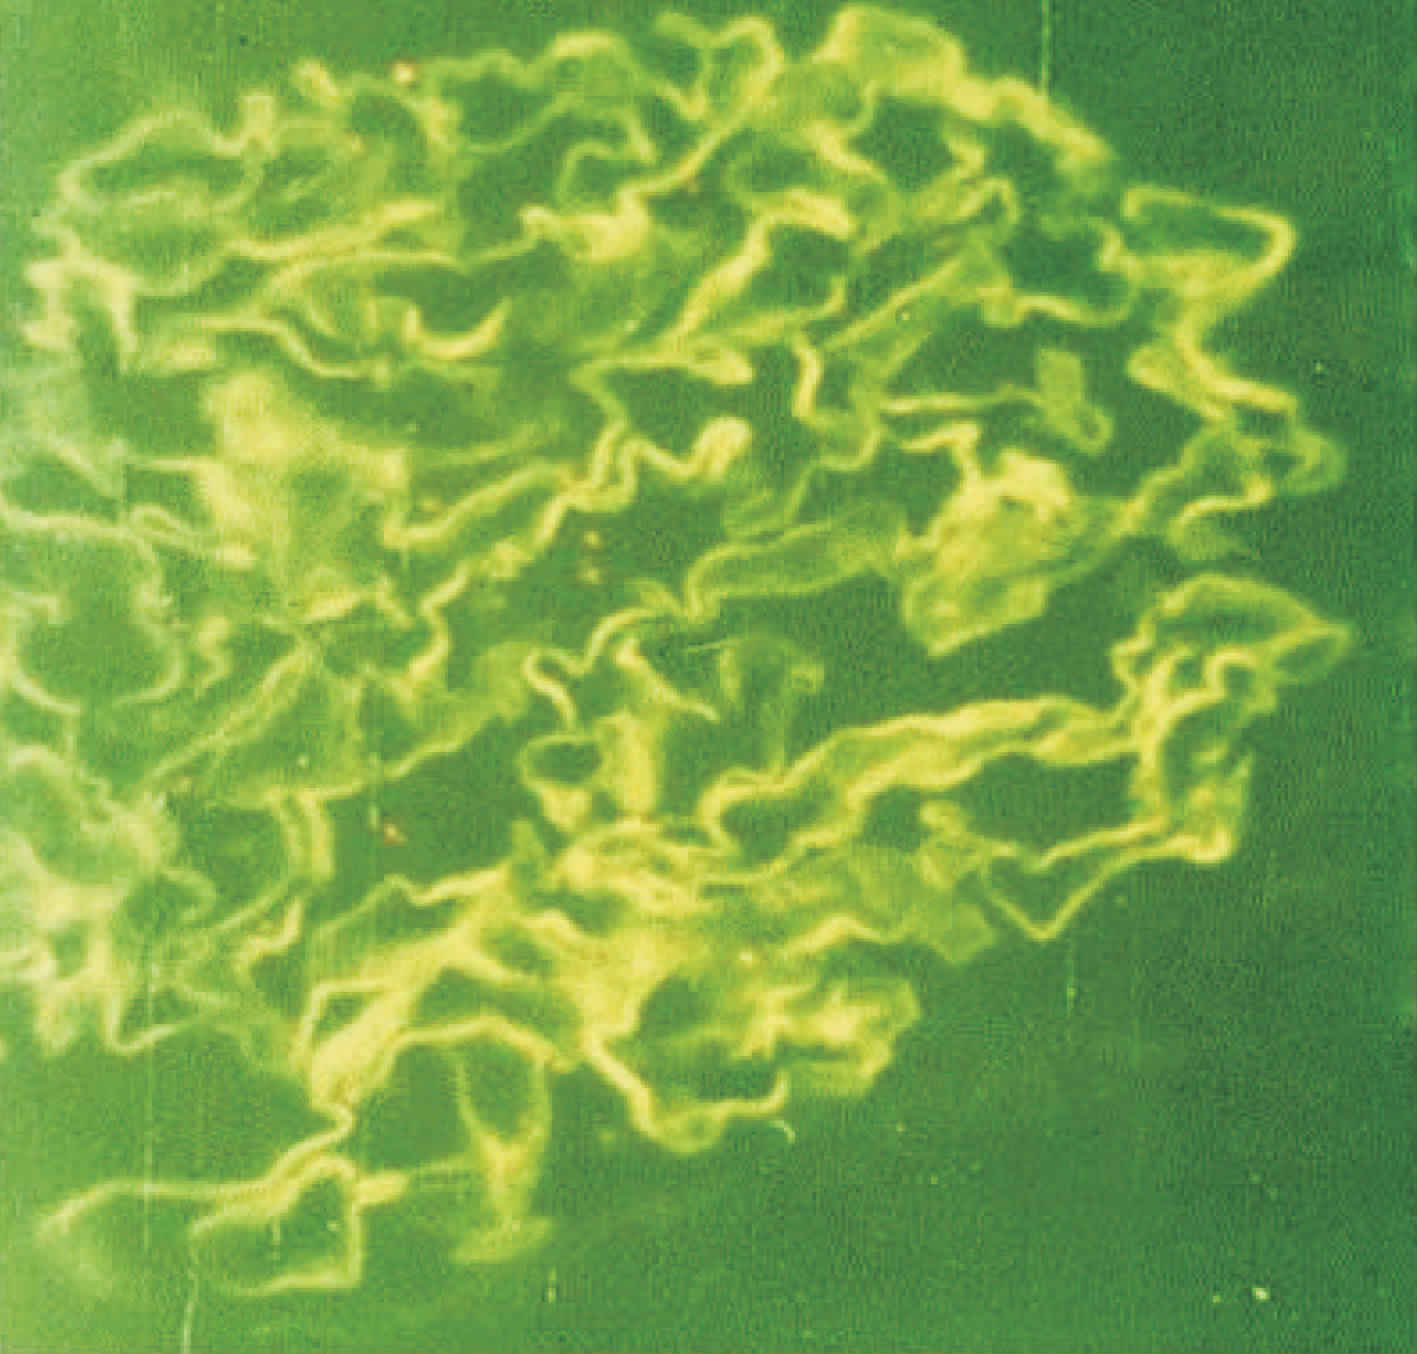
\includegraphics{./images/Image00148.jpg}
 \captionsetup{justification=centering}
 \caption{抗肾小球基膜抗体引起的肾炎\\ {\small 免疫荧光检查显示有特征性的连续的线性荧光}}
\label{fig10-2}
  \end{figure}

(2)Heymann肾炎:这是研究人类原发性膜性肾小球病变的经典的动物模型。复制原理是:由于肾小球脏层上皮细胞足突表面的糖蛋白(即Heymann抗原)与肾小管刷状缘抗原有共同的抗原性,所以当用近曲小管刷状缘成分为抗原免疫大鼠,使大鼠产生抗体,然后抗体与足细胞小凹上的抗原复合物结合,并激活补体,引起与人膜性肾小球病相似的病变,但抗原是否一致尚未确定。电镜检查显示毛细血管基膜与足细胞之间有许多小块状电子致密沉积物。免疫荧光检查显示弥漫的颗粒状分布的免疫球蛋白或补体沉积。

(3)抗体与植入抗原的反应:所谓植入性抗原即指外源性或内源性的植入于肾小球的抗原,是由肾小球以外的成分,随血液流经肾脏时,通过与肾小球成分反应定位于肾小球形成。体内产生的抗体与被植入的抗原反应而非肾小球。免疫荧光检查显示散在的颗粒状荧光。

\paragraph{循环免疫复合物性肾小球肾炎}
机体受刺激后产生的抗体与非肾小球性可溶性抗原在血循环中结合形成抗原抗体复合物(循环免疫复合物),随血液循环沉积于肾小球,并常与补体结合引起肾小球病变(图\ref{fig10-3})。抗原可为内源性的(如核抗原、免疫球蛋白、甲状腺球蛋白等)或是外源性的(如感染因子,包括细菌、病毒和寄生虫等的抗原成分)。在人类的肾小球肾炎中,致病的内源性或外源性抗原常常是未知的。电镜见高密度电子沉积物,可分别定位于系膜区、内皮和基膜间构成内皮下沉积或基膜与足细胞间构成上皮下沉积。免疫荧光检查显示肾小球病变部位有颗粒状免疫荧光,为免疫球蛋白或补体成分(图\ref{fig10-4})。

\begin{figure}[!htbp]
 \centering
 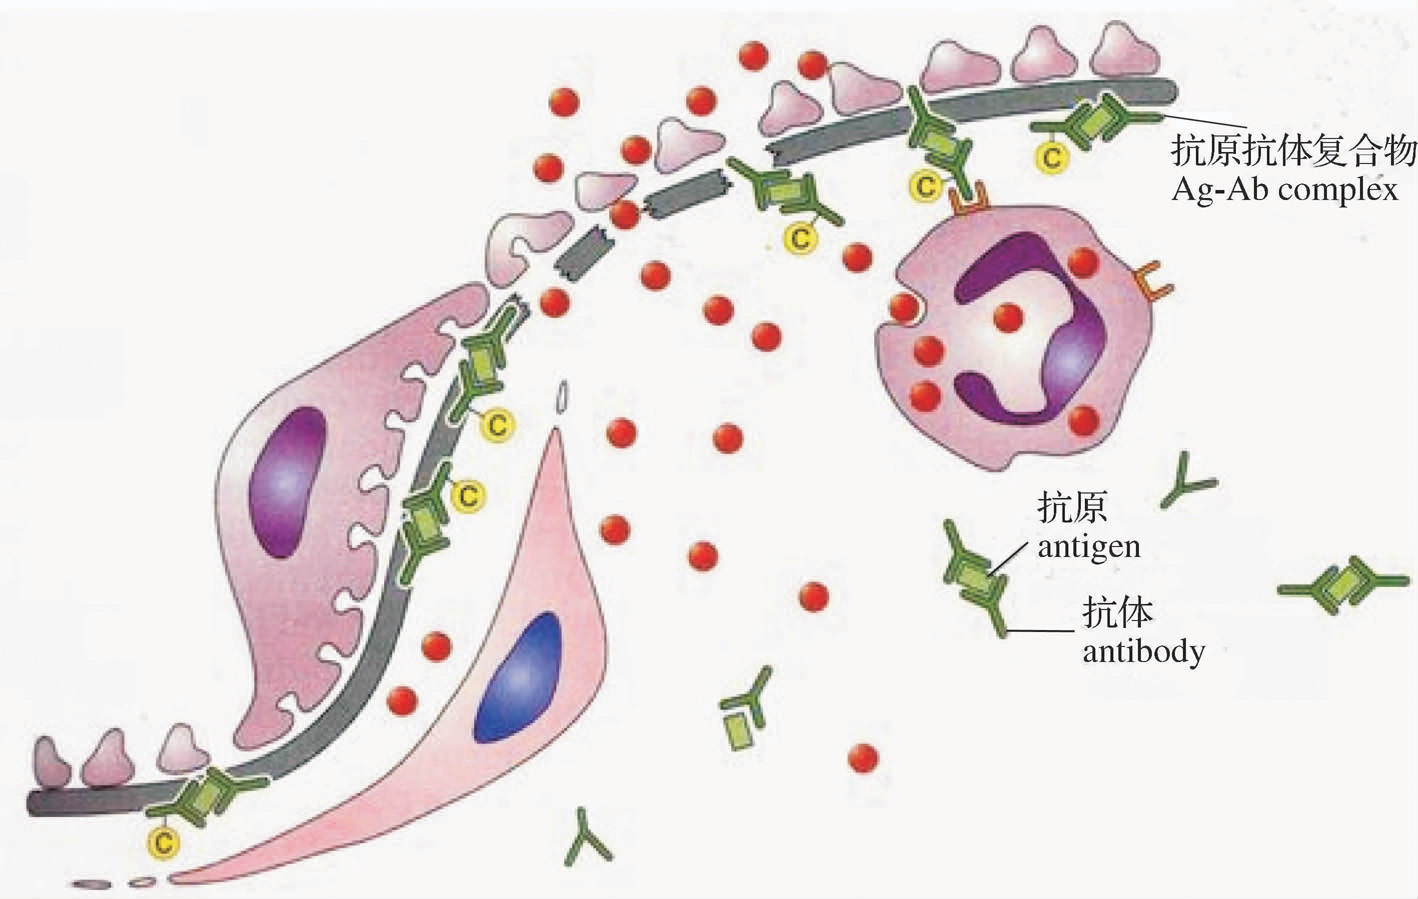
\includegraphics{./images/Image00149.jpg}
 \captionsetup{justification=centering}
 \caption{循环免疫复合物性肾小球肾炎的模式图\\ {\small 机体受刺激后产生的抗体与非肾小球性可溶性抗原在血循环中结合形成抗原抗体复合物(循环免疫复合物),随血液循环沉积于肾小球}}
\label{fig10-3}
  \end{figure}

\begin{figure}[!htbp]
 \centering
 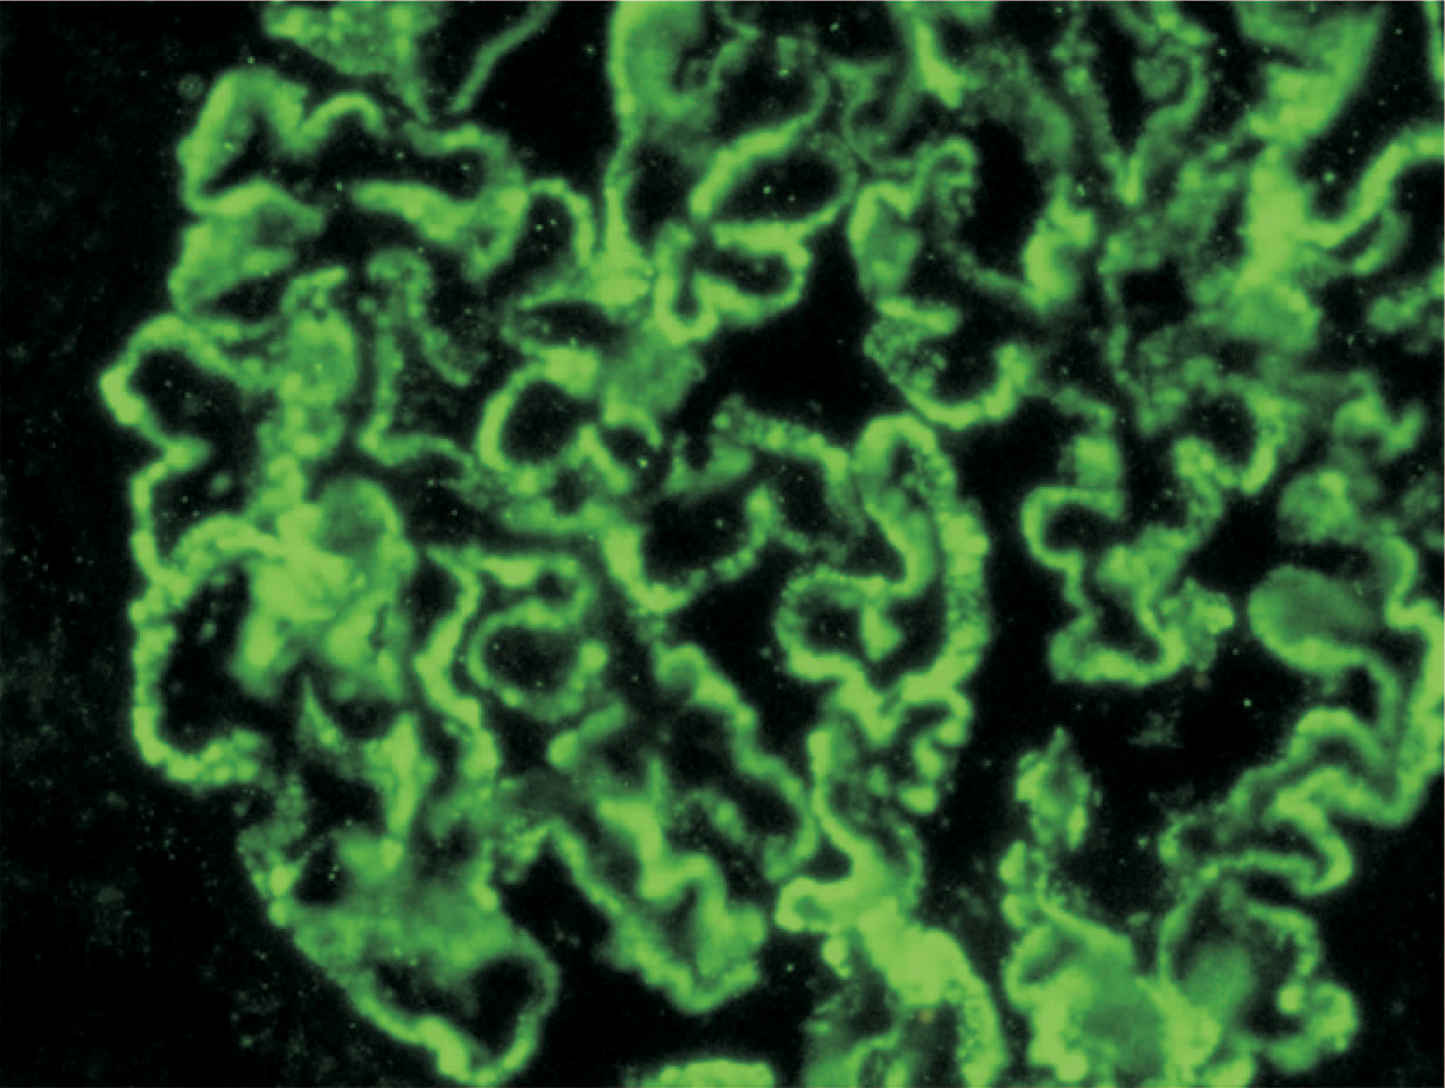
\includegraphics{./images/Image00150.jpg}
 \captionsetup{justification=centering}
 \caption{免疫荧光检查显示沿肾小球毛细血管壁分布之颗粒状荧光}
 \label{fig10-4}
  \end{figure} 

循环免疫复合物是否在肾小球内沉积、沉积的部位和数量受多种因素的影响,其中两个最重要的因素是复合物分子的大小和复合物携带的电荷。大分子复合物常被血液中的吞噬细胞清除,小分子复合物易通过肾小球滤过膜,均不易在肾小球内沉积。含阳离子的复合物可穿过基膜,易沉积于上皮下(毛细血管基膜与脏层上皮细胞之间),含阴离子的复合物不易通过基膜,常沉积于内皮下(毛细血管基膜与内皮细胞之间);电荷中性的复合物易沉积于系膜区。其他影响免疫复合物沉积的因素包括肾小球血流动力学、系膜细胞的功能和滤过膜的电荷状况等。

\paragraph{细胞免疫性肾小球肾炎}
细胞免疫可能是未发现抗体反应的肾炎发病的主要机制。现已证明致敏的T淋巴细胞可引起肾小球损伤,这是因为致敏的T淋巴细胞可释放多种淋巴因子,吸引单核细胞,后者被活化分化成巨噬细胞,除具有吞噬功能外,还能分泌胶原酶、弹性蛋白酶及其他蛋白酶,均能损伤肾小球。

此外,抗肾小球细胞抗体和补体替代途径的激活也可引起肾小球损伤。

\paragraph{肾小球损伤性介质}
肾小球内出现免疫复合物或致敏T淋巴细胞后需有各种介质的参与才能引起肾小球损伤,这些介质包括细胞性(中性粒细胞源性、单核细胞-巨噬细胞-淋巴细胞源性、血小板源性、肾小球源性)和体液来源的大分子可溶性介质(图\ref{fig10-5})。各自功能概括如下:

\begin{figure}[!htbp]
 \centering
 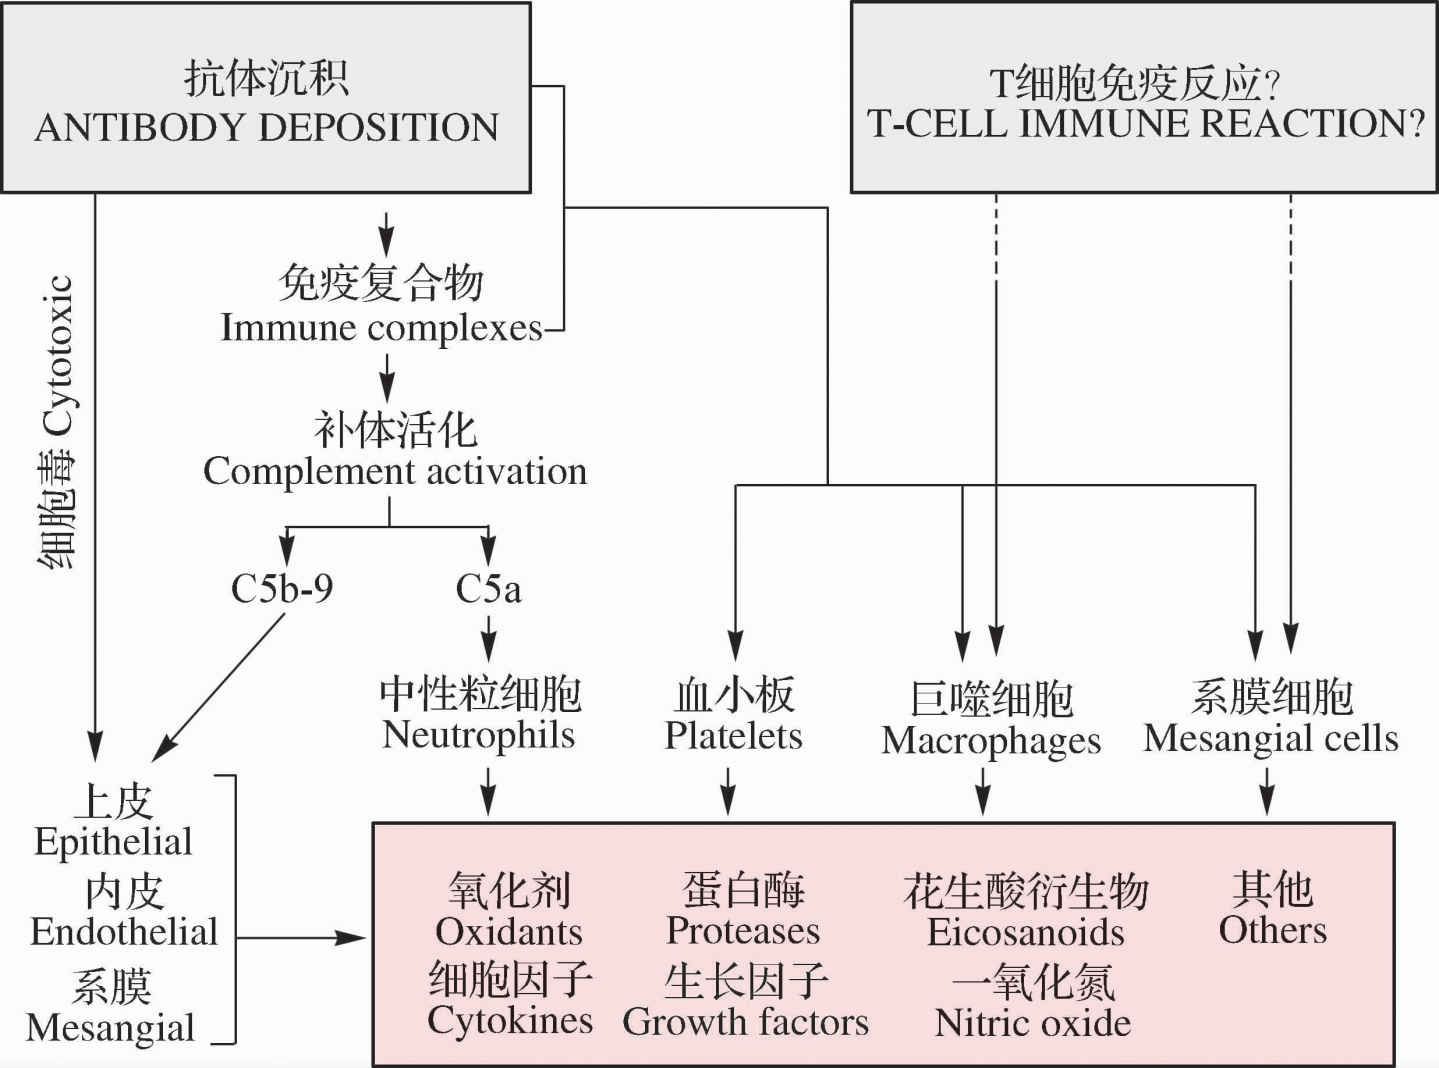
\includegraphics{./images/Image00151.jpg}
 \captionsetup{justification=centering}
 \caption{肾小球损伤的介质}
 \label{fig10-5}
  \end{figure} 

(1)免疫复合物沉积的肾小球疾病中,补体-白细胞介导的机制是引起肾小球病变的一个重要途径。补体激活后产生C5a等趋化因子,引起中性粒细胞和单核细胞浸润。中性粒细胞释放蛋白酶,在补体活化反应区积聚然后释放蛋白酶、花生四烯酸代谢产物和氧自由基。蛋白酶使肾小球基膜降解,氧自由基引起细胞损伤,花生四烯酸代谢产物使肾小球滤过率降低。另一些肾炎病变中炎细胞数量很少,病变则可能由不依赖白细胞的补体依赖性机制引起。如C5b-C9末端膜攻击复合物可引起细胞溶解并刺激肾小球系膜细胞释放复杂的蛋白酶、氧自由基、白细胞介素-1和前列腺素。

(2)在未发现免疫复合物沉积的肾小球疾病中,抗肾小球细胞抗体引起的细胞损伤可能起主要作用。抗体可直接与肾小球细胞的抗原成分反应,通过抗体依赖的细胞毒反应等机制诱发病变。抗系膜细胞抗原的抗体造成系膜溶解,并使系膜细胞增生;抗内皮细胞抗原的抗体引起内皮细胞损伤和血栓形成;抗脏层上皮细胞糖蛋白抗体引起的损伤可导致蛋白尿。

(3)其他引起肾小球损伤的介质 包括:①单核细胞和巨噬细胞:通过抗体或细胞介导的反应浸润至肾小球,被激活时释放大量生物活性物质[细胞中介物、细胞因子(cytokine)和生长因子],加剧肾小球损伤;②血小板:聚集在肾小球内的血小板可释放花生四烯酸代谢物和生长因子等,促进肾小球的炎性改变;③肾小球固有细胞:肾小球固有细胞包括系膜细胞、上皮细胞和内皮细胞,肾小球免疫损伤中生成的多种细胞因子、系膜基质和肾小球基膜降解产物可作用于细胞表面相应的受体,使之激活,并释放多种介质。系膜细胞受炎症刺激时可释放活性氧、细胞因子、趋化因子、花生四烯酸衍生物、一氧化氮和内皮素等。在无炎细胞浸润的情况下,系膜细胞等肾小球固有细胞释放的介质可引起肾小球病变;④凝血蛋白,特别是纤维蛋白,可引起白细胞浸润和肾小球细胞增生,可能是新月体形成的主要刺激物之一。

(4)其他炎性介质 详见炎症章,也可引起肾小球的损伤。

综上所述,肾小球损伤机制的要点为:①抗体介导的免疫损伤是肾小球损伤的重要机制,这一机制主要通过补体和白细胞介导的途径发挥作用;②大多数抗体介导的肾炎由循环免疫复合物沉积引起,免疫荧光检查时,免疫复合物呈颗粒状分布;③抗肾小球基膜成分的自身抗体可引起抗肾小球基膜性肾炎,免疫荧光检查时抗体呈线性分布;④抗体可与植入肾小球的抗原发生反应,导致原位免疫复合物形成,免疫荧光检查显示颗粒状荧光。

\subsubsection{非免疫机制}

不论何种肾脏疾病,肾小球的或是其他方面的,损坏大量的肾单位都会降低肾小球滤过率(glomerular
filtration
rate,GFR)至正常的30%~50%,晚期必然会引起肾小球硬化和肾衰竭(尽管病程不一)。长期的高血压会导致上皮和内皮的损伤,产生蛋白尿。肾小球基膜的变化,包括系膜细胞增生和基质沉积,以及肾小球内的凝固作用将导致肾小球硬化症。肾小球的损害会导致肾功能的进一步丧失和进行性肾小球硬化症的恶性循环。

\subsection{肾小球肾炎的基本病理变化}

不论肾小球疾病的病因是什么,肾小球对损伤的反应主要有以下几种基本病变,肾小球疾病时可出现一种或联合出现几种基本病变,包括:

\paragraph{细胞增多}
表现有肾小球内细胞数目增多(图\ref{fig10-6}),可能与肾小球内系膜细胞、内皮细胞或上皮细胞的增殖有关,或与炎性细胞如中性白细胞或单核细胞的浸润有关。毛细血管内增生指内皮细胞增生,伴或不伴有系膜细胞的增生。而毛细血管外增生指上皮细胞的增生,有利于形成细胞性新月体。细胞增生是潜在可逆的过程。

\begin{figure}[!htbp]
 \centering
 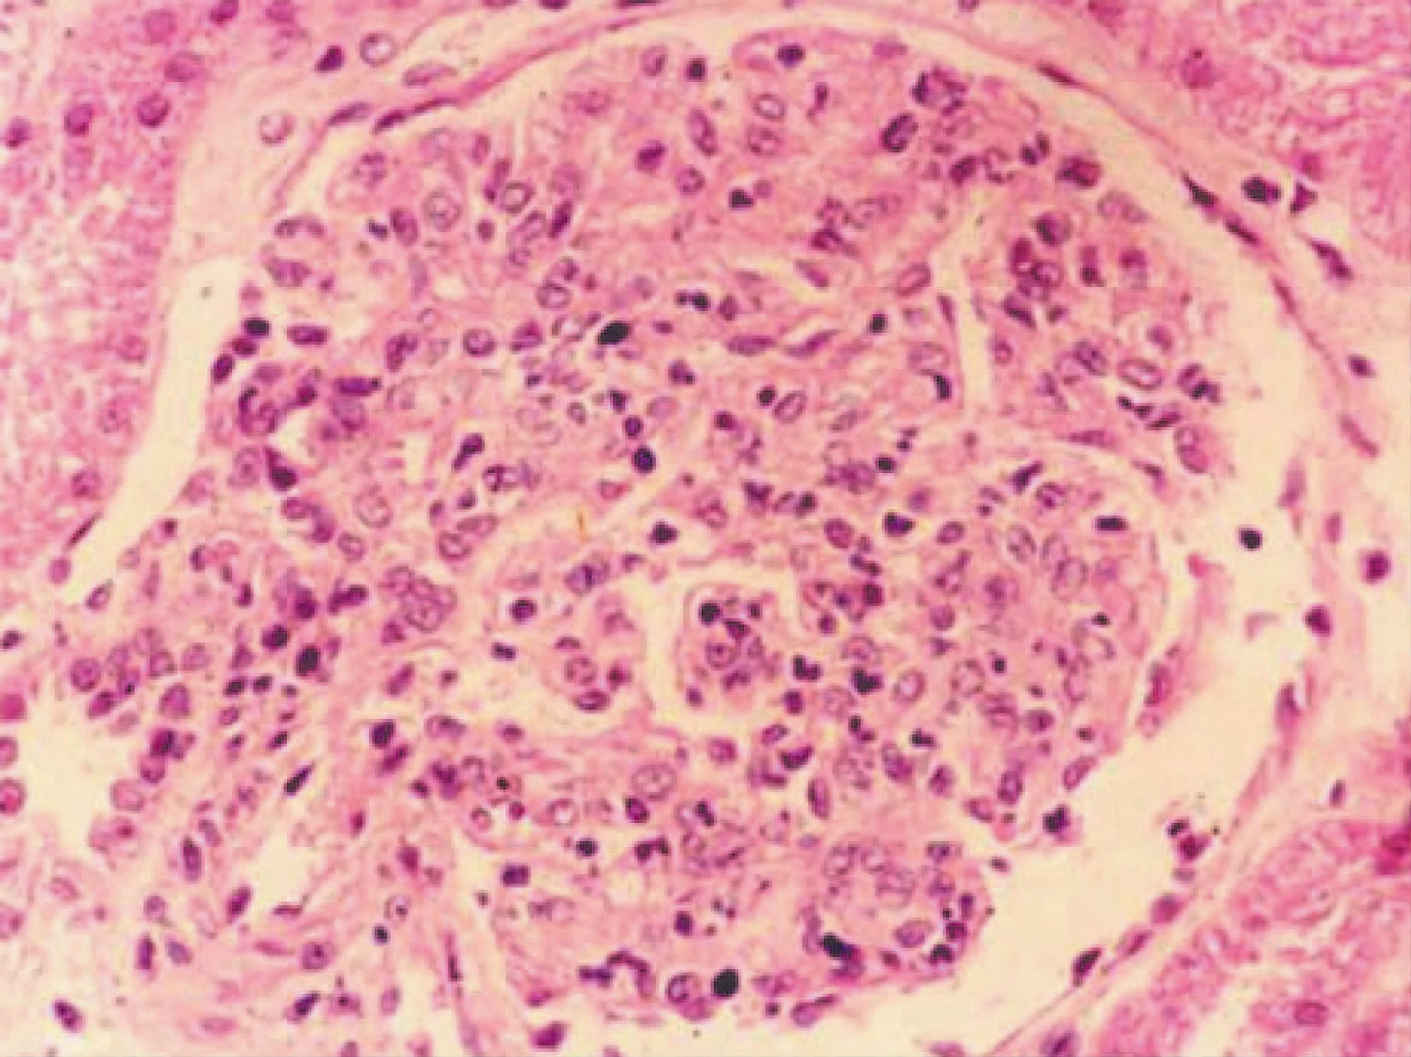
\includegraphics{./images/Image00152.jpg}
 \captionsetup{justification=centering}
 \caption{肾小球肾炎基本病理变化(HE染色,高倍)\\ {\small 肾小球体积增大,其内细胞数目增多,包含有系膜细胞、内皮细胞,炎性细胞浸润如中性粒细胞和单核细胞}}
\label{fig10-6}
  \end{figure}

\paragraph{渗出和坏死}
表现有肾小球内中性白细胞的浸润,纤维蛋白的沉积,毛细血管纤维素样坏死(图\ref{fig10-7})、基膜的断裂,可能伴有血栓形成。病变通常是节段性的(累及肾小球的部分小叶),可能伴有细胞性新月体或被细胞性新月体掩盖。坏死性病变愈合后形成节段性硬化。

\begin{figure}[!htbp]
 \centering
 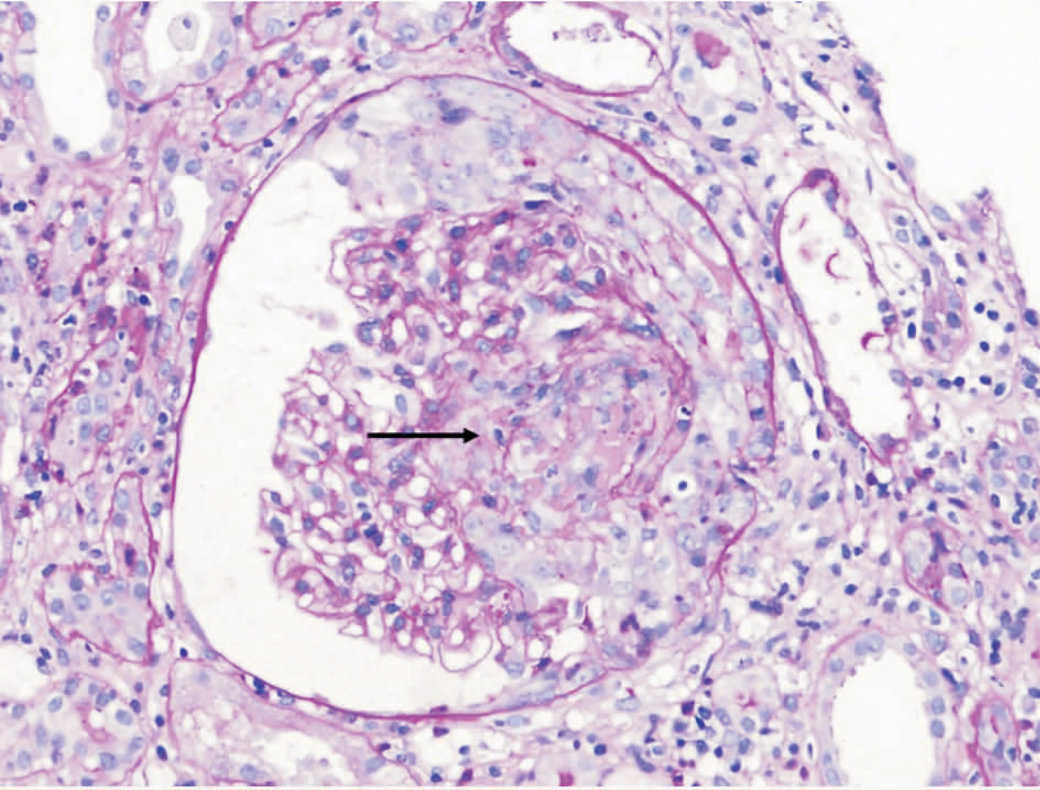
\includegraphics{./images/Image00153.jpg}
 \captionsetup{justification=centering}
 \caption{肾小球肾炎基本病理变化(PAS染色,高倍)\\ {\small 肾小球毛细血管丛节段纤维素样坏死(箭头所示),细胞性新月体形成}}
\label{fig10-7}
  \end{figure}

\paragraph{基膜增厚}
光镜下,过碘酸-Schiff(periodic
acid-schiff,PAS)和过碘酸六亚甲基四胺银(periodic acid-sliver
methenamine,PASM)等染色可显示基膜增厚。电镜观察表明基膜改变可以是基膜本身的增厚,也可为内皮下、上皮下或基膜内免疫复合物沉积。

\paragraph{玻璃样变性和硬化}
肾小球玻璃样变性亦称肾小球硬化,在光镜下呈现非细胞的嗜伊红物质(图\ref{fig10-8}),主要为糖蛋白,与淀粉样物质(图\ref{fig10-9})不易区分。

\begin{figure}[!htbp]
 \centering
 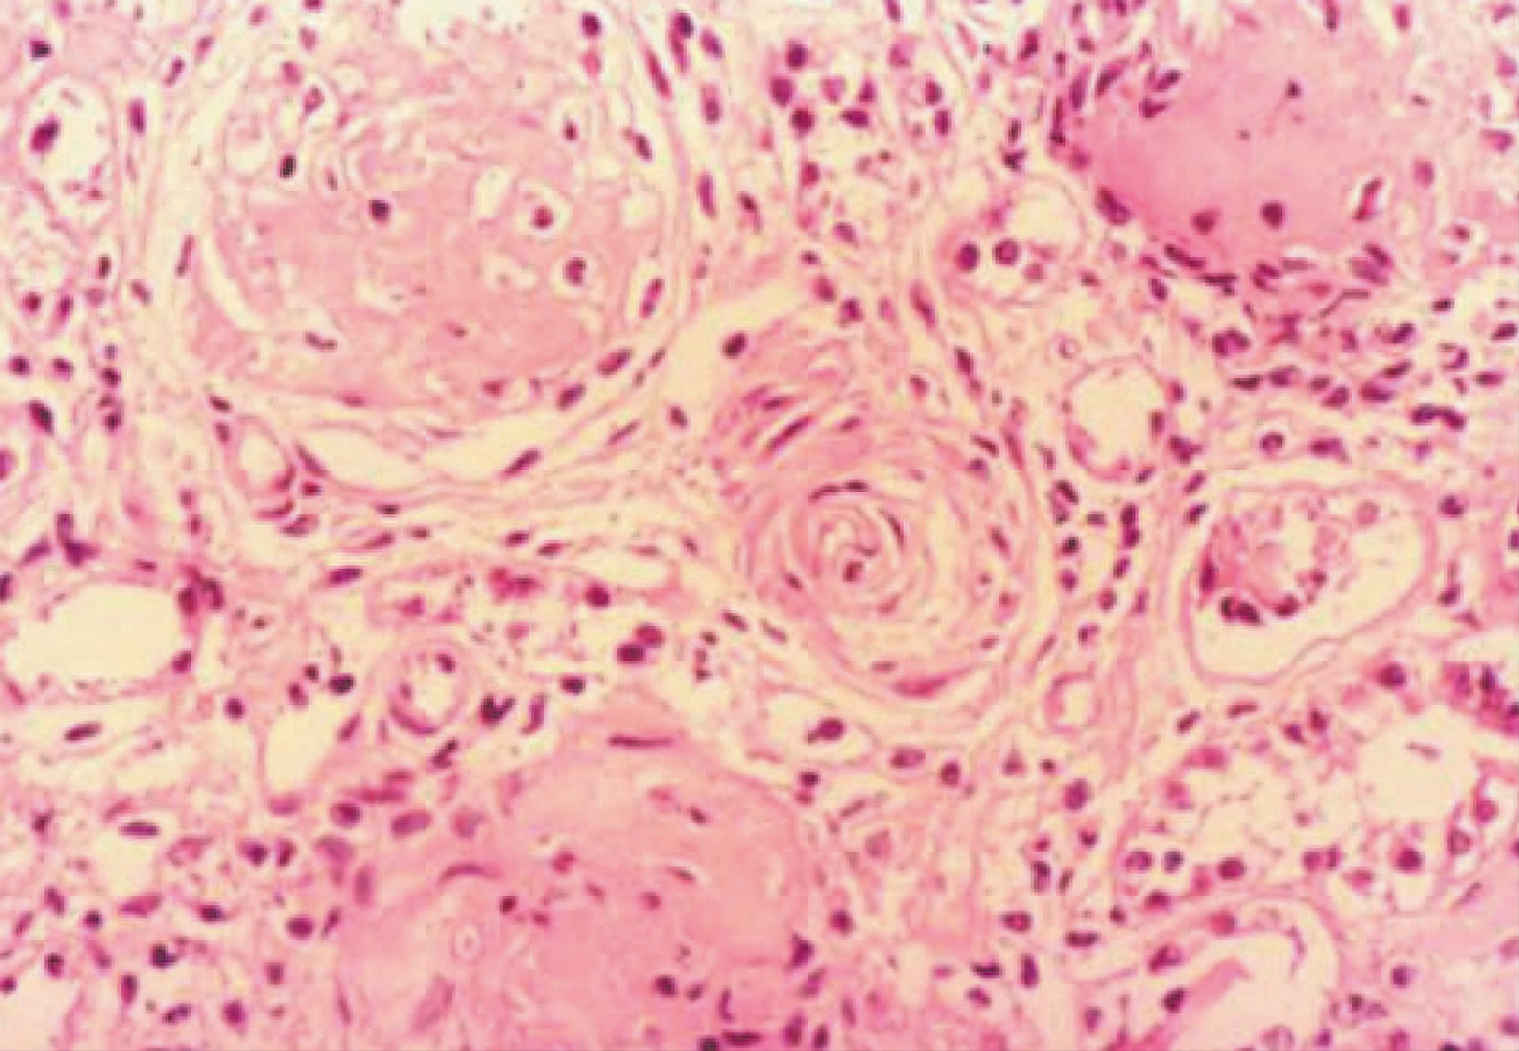
\includegraphics{./images/Image00154.jpg}
 \captionsetup{justification=centering}
 \caption{肾小球玻璃样变性(HE染色,高倍)}
 \label{fig10-8}
  \end{figure} 

\begin{figure}[!htbp]
 \centering
 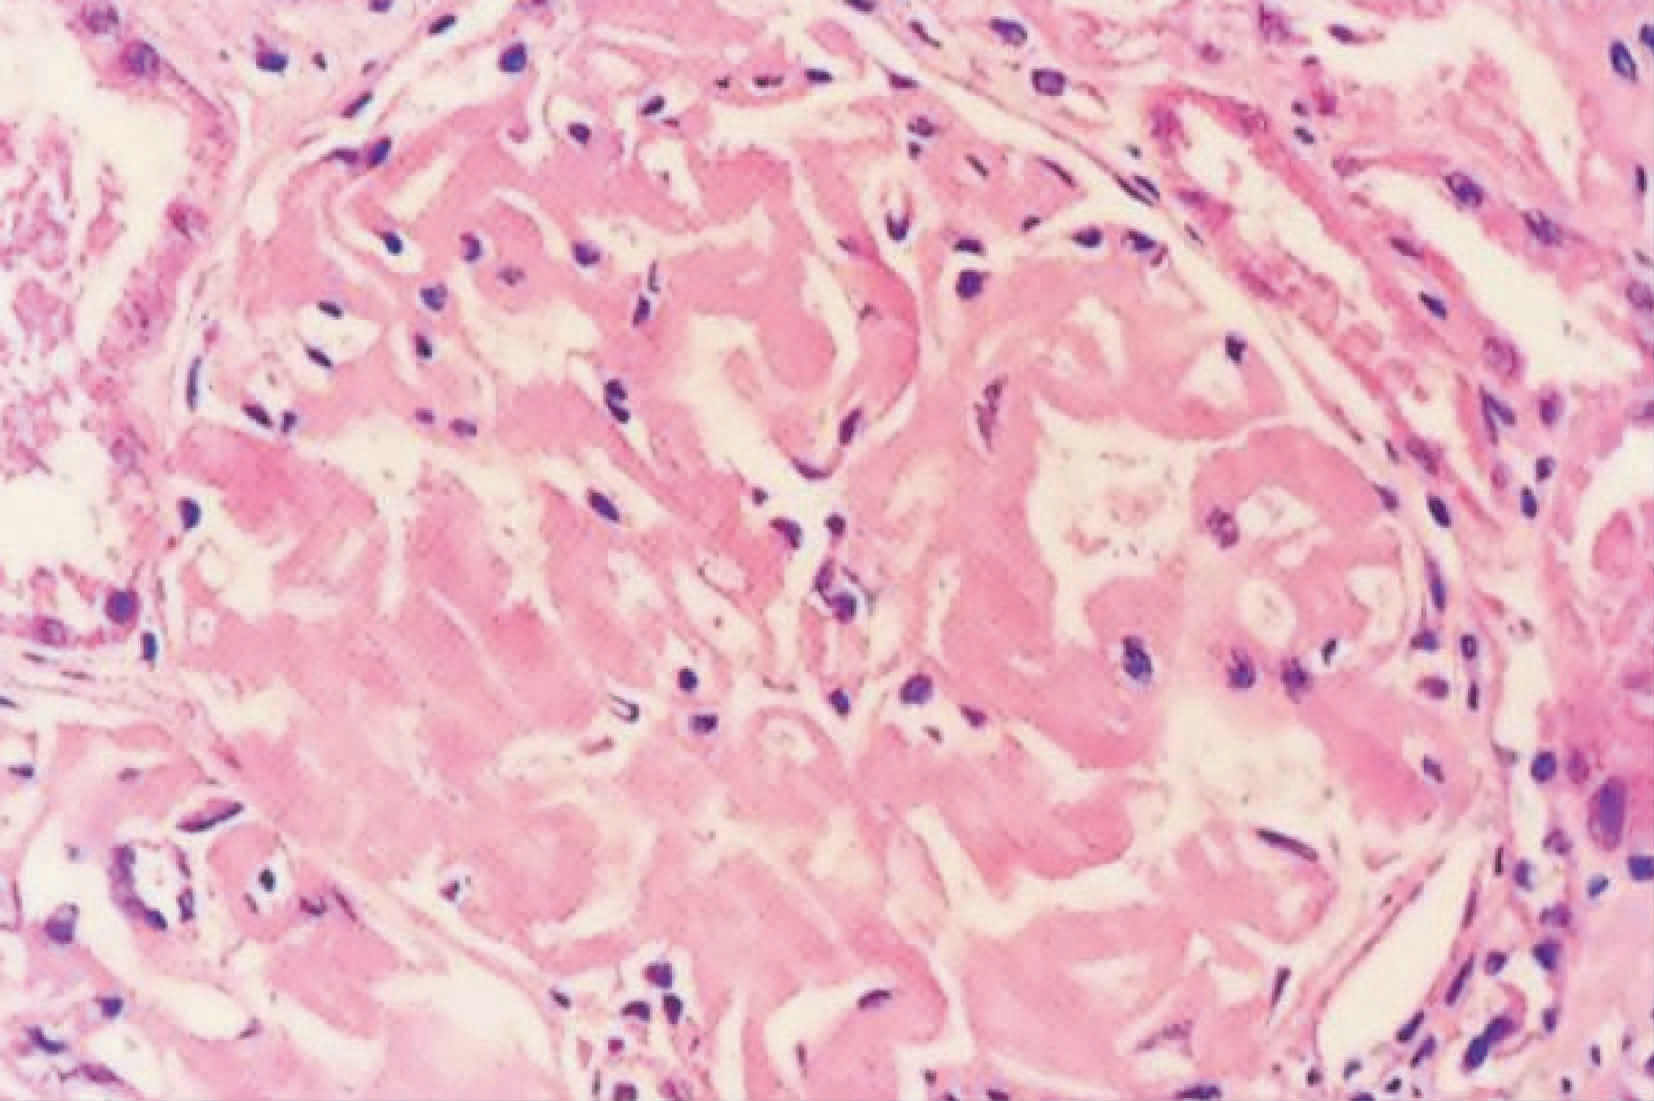
\includegraphics{./images/Image00155.jpg}
 \captionsetup{justification=centering}
 \caption{肾小球内淀粉样物质沉积(HE染色,高倍)}
 \label{fig10-9}
  \end{figure} 

电镜下见细胞外出现无定形物质,可为沉积的血浆蛋白、增厚的基膜和增多的系膜基质。胶原纤维进一步增加则肾小球固有细胞减少甚至消失,最终导致节段性或整个肾小球的硬化,这是一个不可逆过程,常伴有泡沫细胞黏附到鲍曼囊(Bowman's
capsule)壁。PAS或PASM染色能很好地显示硬化,借此可将硬化与纤维化相鉴别,纤维化时PAS或PASM染色呈阴性。透明变性和淀粉样物的鉴别则依赖特殊染色或超微结构。

\paragraph{肾小管和间质的改变}
继发于肾小球玻变和硬化,相应肾小管萎缩或消失,肾间质可不同程度地充血、水肿、炎细胞浸润和纤维化。若肾小管上皮细胞变性,肾小管腔内还可能出现蛋白质管型、细胞管型或颗粒管型。

肾穿刺活检标本的光镜学检查是肾脏疾病常用的病理学检查方法,相应的组织切片染色除常规苏木素伊红(HE)染色外,更常借助PAS染色、PASM和Masson三色染色等特殊染色法。PAS染色可显示基膜和系膜基质,PASM对基膜的染色更为清晰;Masson染色可显示特殊蛋白性物质(包括免疫复合物),也可显示胶原纤维等。此外,还可用Fibrin染色显示血栓和纤维素样坏死。肾活检组织还常规运用免疫荧光法检查免疫球蛋白(IgG,IgM,IgA)和补体成分(C3,C1q和C4)沉积。透射电镜被用以观察超微结构改变和免疫复合物沉积的状况及部位。

\subsection{肾小球肾炎的主要临床表现}

肾小球肾炎的临床症状主要包括尿量、尿性状的改变、水肿和高血压等表现。尿量的改变有少尿、无尿、多尿或夜尿。若24小时尿量少于400
ml则为少尿,其中少于100 ml为无尿,若24小时尿量超过2 500
ml则为多尿。尿性状的改变有血尿、蛋白尿和管型尿。血尿分为肉眼血尿和显微镜下血尿。尿中蛋白含量每天超过150
mg为蛋白尿,每天超过3.5
g则为大量蛋白尿。管型由蛋白质、细胞或细胞碎片在肾小管凝集形成,尿中出现大量管型称为管型尿。若肾小球滤过率下降,血尿素氮和血浆肌酐水平增高,则形成氮质血症。尿毒症可发生于各型肾炎晚期,除氮质血症的表现外,还具有一系列自体中毒的症状和体征,常出现胃肠道、神经、肌肉和心血管等系统的病理改变,如尿毒症性胃肠炎、周围神经病变、纤维素性心外膜炎等。急性肾衰竭表现为少尿和无尿,并出现氮质血症。慢性肾衰竭表现为多尿、夜尿、低比重尿,和持续出现的尿毒症。

肾小球肾炎的临床表现因不同的病理类型而出现上述不同的症状和体征,二者既密切联系又非完全对应,而且疾病的病程、病变性质和程度也常使疾病呈现不同的临床表现。肾小球肾炎患者所表现出来的这种具有一定结构和功能联系的症状组合,即为综合征。不同的肾小球肾炎具有的综合征可概括如下:

\paragraph{急性肾炎综合征}
起病急,肉眼血尿、蛋白尿、水肿和高血压,肾小球滤过率降低伴氮质血症。见于急性弥漫性肾小球肾炎。因少尿使机体代谢产物排出受阻,结果血中尿素氮、肌酐等非蛋白氮含量增高称氮质血症。

\paragraph{急进性肾炎综合征}
起病急,肉眼血尿、水肿、蛋白尿,迅速进展的少尿或无尿,氮质血症和快速进行性肾衰竭,可伴贫血。见于急进性肾小球肾炎。

\paragraph{肾病综合征}
大量蛋白尿,每天尿中蛋白含量超过3.5
g;严重水肿、低蛋白血症、高脂血症和脂尿。见于多种类型的肾小球肾炎。

\paragraph{无症状性血尿或蛋白尿}
持续或复发性肉眼或镜下血尿,和(或)轻度蛋白尿。多见于IgA肾病。

\paragraph{慢性肾炎综合征}
慢性进行性,多尿、夜尿、低比重尿,可伴血尿、蛋白尿、高血压、贫血、氮质血症和尿毒症。见于慢性肾小球肾炎。

\subsection{肾小球肾炎的病理类型}

肾小球肾炎可分为原发性和继发性,原发性是指病因不明和(或)主要累及肾小球的病变。继发性肾小球肾炎指肾小球病变与已知的系统性疾病有关,在继发性病变中病变可以以肾小球病变为主,也可以以其他病变为主。有些疾病如IgA肾病由于对它的发病机制还不完全理解,可能有其他的分类标准。

由于原发性肾小球肾炎的病因不明,因此该病主要根据各自的形态学特点来分类。原发性肾小球肾炎的主要病理类型包括:急性弥漫性增生性肾小球肾炎;急进行性(新月体)肾小球肾炎;膜性肾小球病(膜性肾病);轻微病变性肾小球病(脂性肾病);局灶性节段性肾小球硬化;膜性增生性(系膜毛细血管性)肾小球肾炎;IgA肾病(Berger病);慢性肾小球肾炎。

继发性肾小球肾炎是根据相关的病因或系统性疾病进行分类。如狼疮性肾炎提示肾小球病变与系统性红斑狼疮相关。继发性肾小球肾炎的一些分类可进一步进行亚分类,如代谢性肾小球疾病包括特征性的糖尿病性肾小球硬化、淀粉样物沉积、多发性骨髓瘤、冷球蛋白血症、肝疾病等。

WHO规定以下术语可用于肾小球疾病的分类。由于术语很好地反映了形态学特点,有实用价值。

(1)局灶性:基本病变累及部分但不是所有肾小球(<50%);

(2)弥漫性:基本病变累及到所有或几乎所有肾小球(>50%);

(3)节段性:基本病变累及肾小球的部分毛细血管襻(不超过肾小球切面的50%);

(4)球性:基本病变累及整个肾小球的全部或大部分毛细血管襻。

\begin{framed}
{案例10-1}

{【病例摘要】}

令××,女性,16岁。近3天全身水肿,小便呈酱油色。2周前曾“感冒”一次。血压140/100
mmHg。实验室检查:蛋白尿2+,血清白蛋白32
g/L;尿沉渣红细胞3+。肾穿刺检查发现肾小球内皮细胞、系膜细胞增生以及中性粒细胞浸润;局灶节段肾小球毛细血管壁纤维素样坏死,约20%肾小球有新月体形成;肾小管上皮细胞颗粒变性和玻璃样变,腔内偶见红细胞管型;间质充血。免疫荧光检查显示沿肾小球毛细血管壁分布的颗粒状荧光。

{【问题】}

(1)试问本病最可能的诊断是什么?

(2)为什么会出现全身水肿?
\end{framed}

\subsubsection{急性弥漫性增生性肾小球肾炎}

急性弥漫性增生性肾小球肾炎(acute diffuse proliferative
glomerulonephritis),以包括双肾所有肾小球在内的急性炎症、弥漫性毛细血管内皮细胞和系膜细胞增生、中性粒细胞和巨噬细胞浸润为特征。因减少了肾小球的滤过率,所以又称毛细血管内增生性肾小球肾炎,临床简称急性肾炎。因多数病例发生于溶血性链球菌感染后,因此又称为感染后肾小球肾炎。根据感染病原体的类型,又分为链球菌感染后性肾炎和非链球菌感染性肾炎。前者较为常见。后者由肺炎球菌、葡萄球菌等细菌和腮腺炎、麻疹、水痘和乙型肝炎等病毒引起。

本病主要表现为急性肾炎综合征,好发于儿童和青年,男性比女性更多见,是临床预后较好的肾炎类型。

\paragraph{病因和发病机制}
本型肾炎主要由感染引起,常发生于A族乙型溶血性链球菌(致肾炎菌株12、4、1型)感染后1~4周,与抗体和免疫复合物形成时间相符,同时患者血清抗链球菌溶血素“O”和抗链球菌其他抗原的滴度增高,说明患者近期链球菌的感染史。患者血清补体水平降低,说明有补体的激活和消耗。但肾小球内并不存在链球菌。免疫学、免疫荧光和电镜研究表明此病由循环免疫复合物的沉积引起,免疫球蛋白呈颗粒状“满天星”分布或在上皮下呈“驼峰状”沉积。

\paragraph{病理变化}
(1)肉眼观:双肾轻到中度肿大,被膜紧张,表面充血,故称大红肾,有时肾表面见散在粟粒状的出血点,故又有蚤咬肾之称(图\ref{fig10-10})。切面见肾皮质增宽,有小出血点。

\begin{figure}[!htbp]
 \centering
 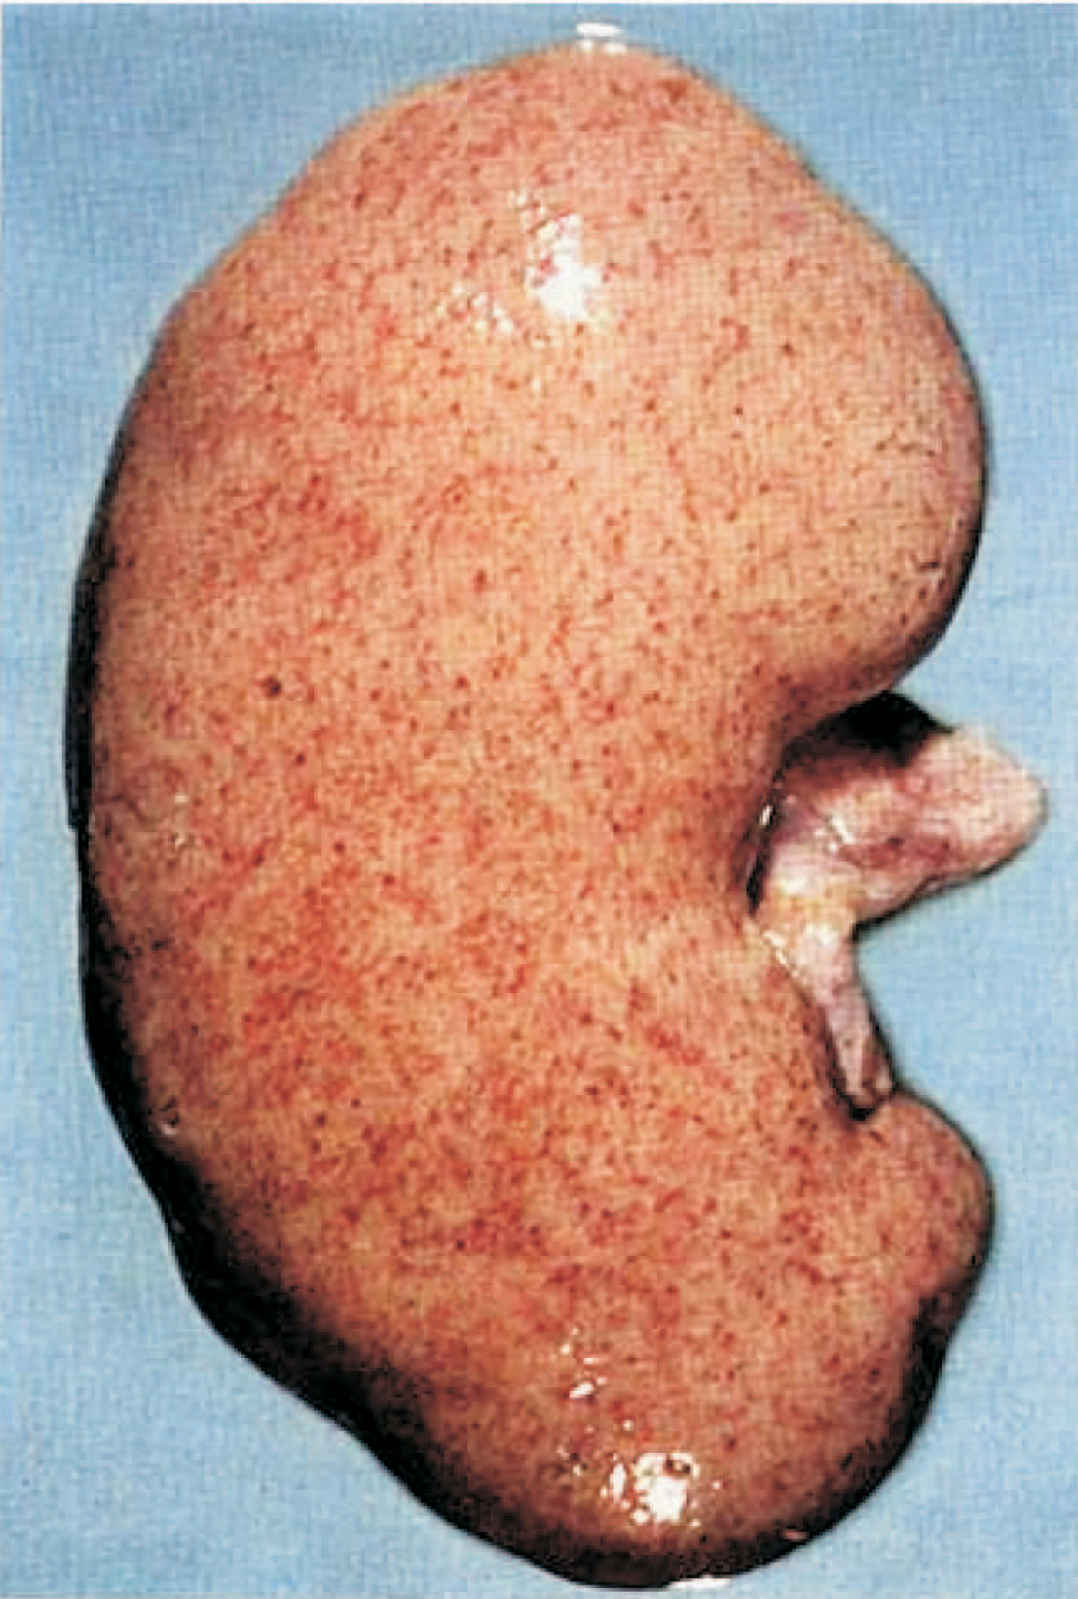
\includegraphics{./images/Image00156.jpg}
 \captionsetup{justification=centering}
 \caption{急性弥漫性增生性肾小球肾炎\\ {\small 大体见肾脏充血肿大,被膜紧张,表面可见散在粟粒状的出血点(蚤咬肾)}}
\label{fig10-10}
  \end{figure}

(2)光镜下:HE显示双肾大多数肾小球广泛受累。肾小球体积增大,毛细血管丛的细胞数明显增多(即球高细胞性),主要是由于内皮细胞、系膜细胞明显增生,伴中性粒细胞和单核细胞浸润所致(图\ref{fig10-11})。受增生细胞的充填和挤压,毛细血管腔及肾小球囊狭窄或闭塞,肾小球血量减少。病变严重的病例,毛细血管壁可发生节段性纤维素样坏死,局部出血,可伴血栓形成。在某些病例中,少数肾小球可显示沿鲍曼囊排列的上皮细胞增生,并伴早期“新月体”形成。

\begin{figure}[!htbp]
 \centering
 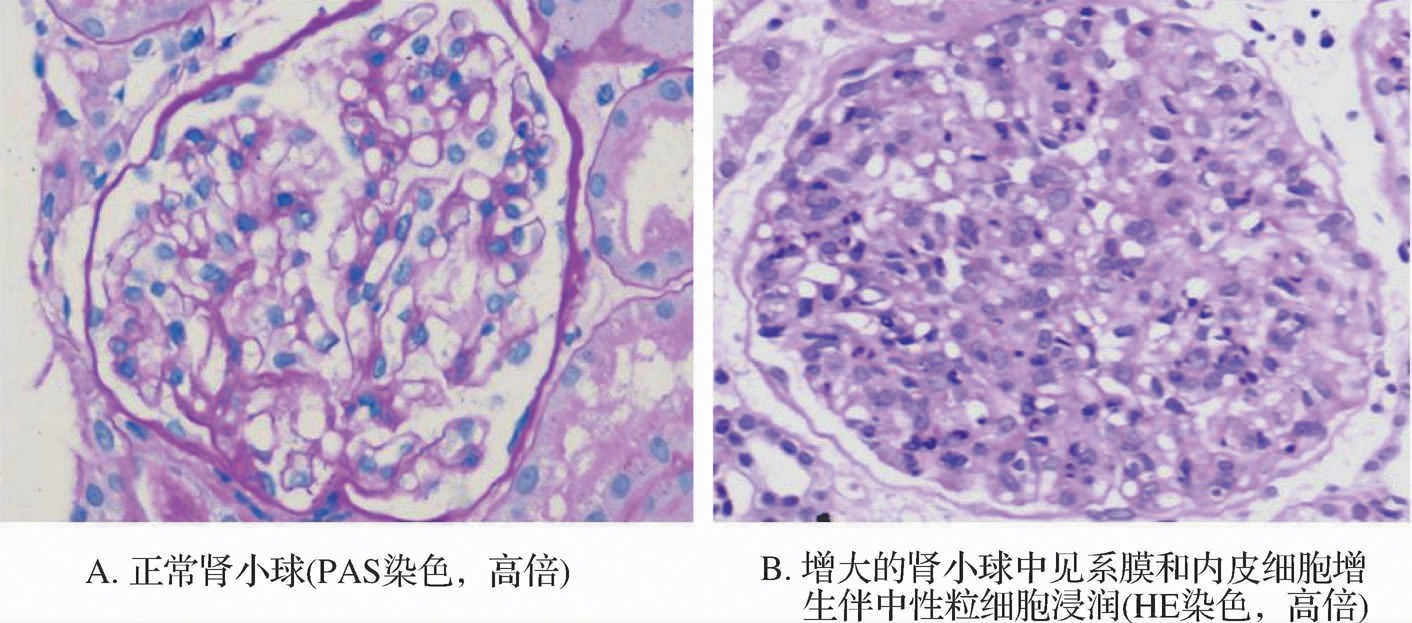
\includegraphics{./images/Image00157.jpg}
 \captionsetup{justification=centering}
 \caption{急性弥漫性增生性肾小球肾炎}
 \label{fig10-11}
  \end{figure} 

肾小管改变不如肾小球明显,但是炎症严重时可发生小管扩张、上皮细胞水肿、细胞内玻璃样变性(透明小滴变性)或脂肪样变性,严重者发生坏死。部分肾小管管腔内出现蛋白管型、红细胞或白细胞管型及颗粒管型。肾间质常有不同程度的充血、水肿和少量淋巴细胞、中性粒细胞浸润。

(3)电镜下:见电子密度较高的沉积物,通常呈驼峰状(图\ref{fig10-12}A),多位于上皮下(脏层上皮细胞和肾小球基膜之间),也可位于内皮细胞下、基膜内或系膜区。

\begin{figure}[!htbp]
 \centering
 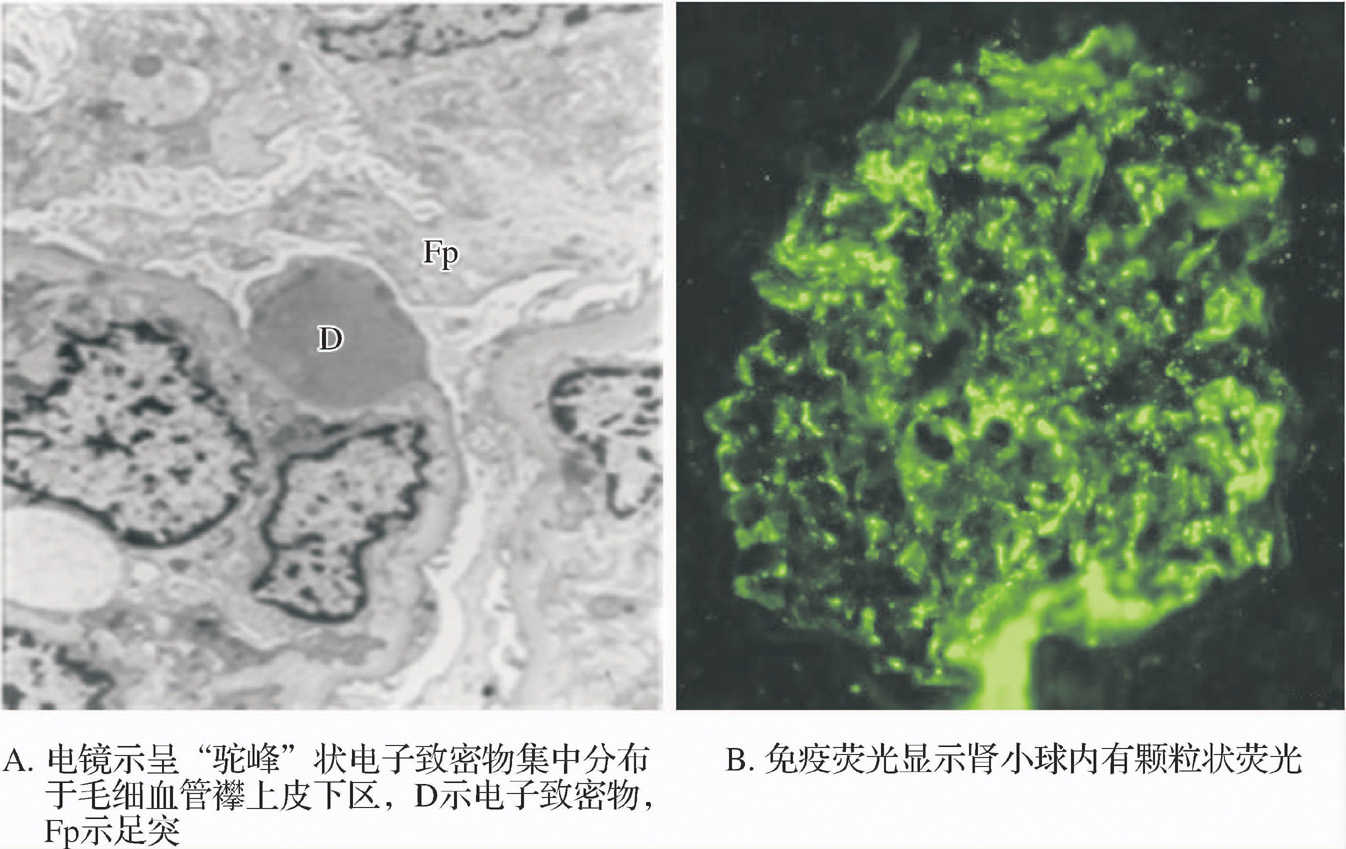
\includegraphics{./images/Image00158.jpg}
 \captionsetup{justification=centering}
 \caption{急性弥漫性增生性肾小球肾炎}
 \label{fig10-12}
  \end{figure} 

(4)免疫荧光:检查显示肾小球内有颗粒状IgG,IgM和C3沿毛细血管襻分布(图\ref{fig10-12}B)。

\paragraph{临床病理联系}
急性肾炎综合征:即由急性发作所致的以肾小球症状占优势。表现有血尿、轻-中度蛋白尿、各种管型(红细胞管型为主),少尿、水肿、高血压,常伴血尿素氮增高。

蛋白尿、血尿、管型尿是因为肾小球损伤、滤过膜通透性增加所致。蛋白尿一般较轻。血尿多为镜下血尿;约30%呈肉眼血尿,常常描述为烟色、赭色或红褐色(酱油色)(由于红细胞释放的血红蛋白在酸性尿中变成血黄质所致),严重血尿可因肾小球毛细血管壁发生纤维素样坏死、出血所致。

少尿是因为毛细血管丛的细胞增生及炎细胞浸润致毛细血管腔狭窄,血流减少,滤过率下降,但肾小管重吸收功能正常,因而少尿甚至无尿。

水肿为最初症状,轻症早期为眼睑水肿,重者波及全身。主要原因是肾小球滤过率降低,水、钠潴留。超敏反应引起的毛细血管通透性增高可使水肿加重。

高血压的原因可能是钠、水潴留,血容量增加。病人的血管神经兴奋性增高也可能起作用,但血浆肾素水平一般不增高。成人患者的症状不典型,可表现为高血压和水肿,常伴有血尿素氮增高。

\paragraph{预后}
95%以上的患病儿童能康复,尤其儿童链球菌感染后肾小球肾炎预后更好,约1%的患儿迁延不愈或发展为快速进行性肾小球肾炎,极少数进展为慢性肾衰竭。在成人,以流行病模式发病的有较好的预后,但以散发模式发病的仅有60%康复,余下者进展为快速进行性肾小球肾炎、慢性肾衰竭。

\subsubsection{急进性(新月体性)肾小球肾炎}

急进性(新月体性)肾小球肾炎(rapidly progressive or crescentic
glomerulonephritis)是一种临床较为少见的肾小球肾炎,可发生于任何年龄组,成人多见。临床上起病急,发展快速,以快速进行性肾小球肾炎综合征为主要表现,并通常在数周至数月内发展成肾衰竭而死亡。主要病理特征为大多数肾小球的鲍曼氏囊腔内细胞积聚,形成“新月体”(crescent)。

\paragraph{病因和发病机制}
新月体性肾小球肾炎为一组由不同原因引起的疾病,可原发于感染后,也可继发于全身性疾病,更多见于特发性原因不明。相应的发病也各有差异,但多数由免疫机制引起。临床常根据免疫学和病理学检查结果,将其病变分为三个类型(表\ref{tab10-1})。

\begin{longtable}[ht]{lll}
    \caption{新月体性肾小球肾炎的分类}
    \label{tab10-1}\\
    \toprule
    I型(抗GBM抗体性)&Ⅱ型(免疫复合物性)&Ⅲ型(免疫反应缺乏性)\\
    \midrule
    \endhead
    原发性&原发性&ANCA相关性\footnote{抗中性粒细胞胞质抗体}\\
Goodpasture综合征&感染后性&原发性\\
&系统性红斑狼疮&Wegener肉芽肿病\\
&过敏性紫癜&显微型结节性多动脉炎/显微型多血管炎\\
&其他&\\
    \bottomrule
\end{longtable}

Ⅰ型为抗肾小球基膜性肾炎。免疫荧光检查呈特征性的线性荧光,主要为IgG沉积,少部分伴有C3沉积。一些病人的抗GBM抗体还与肺泡壁基膜发生交叉反应,引起肺出血-肾炎综合征。病人血清中可检出抗GBM抗体,血浆置换疗法可清除循环血液中的抗体。

Ⅱ型为免疫复合物性肾炎,我国较常见。可发生在链球菌感染后、系统性红斑狼疮、IgA肾病及过敏性紫癜等引起的免疫复合物性肾炎中。免疫荧光检查呈颗粒状荧光,电镜见高密度电子致密物。血浆置换通常无效。

Ⅲ型又称为免疫反应缺乏型肾炎。电镜和免疫荧光检查均呈阴性。主要表现为大部分病人血清内可检出抗中性粒细胞胞质抗体。该抗体与某些类型血管炎的发生有关。本型可以是Wegener肉芽肿病或显微型多动脉炎等系统性血管炎的组成部分。但许多病例的病变局限于肾脏,有的学者认为此类病变由局限于肾小球的血管炎引起。

三种类型中约有50%的病例为原发性病因不明,其余病例与已知的肾脏和肾外疾病有关。三种类型的共同特点是有严重的肾小球损伤。

\paragraph{病理变化}
(1)肉眼观:双肾对称性肿大,柔软,色苍白,有“大白肾”之称,表面可不光滑甚至有点状出血。切面皮质增厚。

(2)光镜下:超过50%肾小球囊内有新月体形成。新月体是肾小球肾炎的一种严重病变,是由于肾小球基膜的灶性损伤处渗出的纤维素等刺激了球囊壁层上皮细胞,使其增生成层,状如新月,故称之。若围绕肾球囊呈环状,则称环状体。新月体主要由增生的壁层上皮细胞和渗出的单核细胞构成,可伴有纤维素以及中性粒细胞和淋巴细胞浸润。早期新月体以细胞成分为主,称为细胞性新月体,或称上皮性新月体(图\ref{fig10-13}A);之后在单核细胞分泌转化生长因子、成纤维细胞生长因子等的作用下,上皮细胞可转分化为成纤维细胞,产生胶原纤维渐增多,转变为纤维-细胞性新月体(图\ref{fig10-13}B);最终完全被纤维所取代,成为纤维性新月体。新月体可使肾小球球囊腔变窄或闭塞,并压迫毛细血管丛,使肾血流量减少,肾小球滤过率下降。部分病人肾小球可分别出现节段性坏死、弥漫或局灶性内皮细胞增生或系膜细胞增生等改变。

\begin{figure}[!htbp]
 \centering
 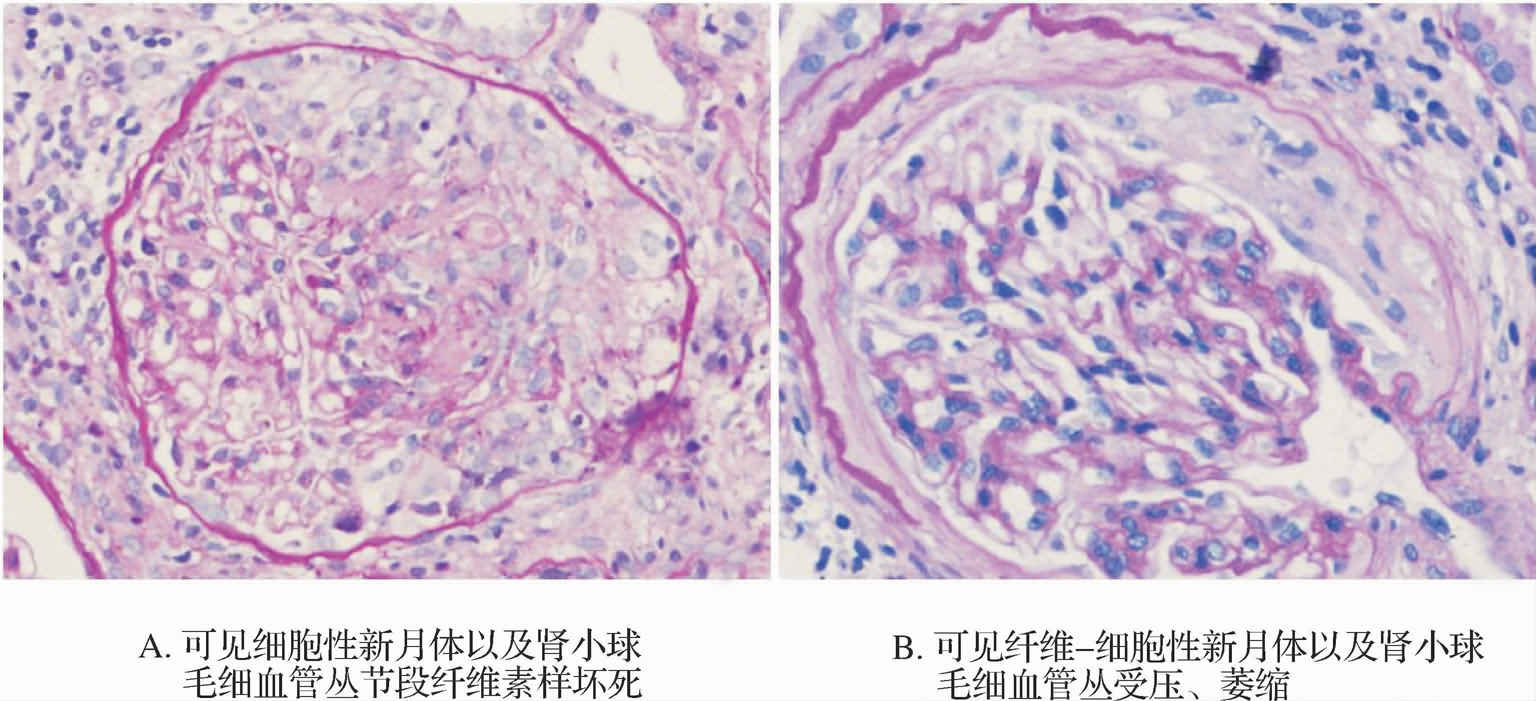
\includegraphics{./images/Image00160.jpg}
 \captionsetup{justification=centering}
 \caption{新月体性肾小球肾炎(PAS 染色,高倍)}
 \label{fig10-13}
  \end{figure}

肾小管上皮细胞可因缺血而出现细胞水肿,因蛋白被吸收而形成细胞内玻璃样变。严重时肾小管上皮细胞可萎缩、坏死甚至消失。肾间质常水肿,炎细胞浸润和纤维化。

(3)电镜下:见新月体,基膜局灶性缺损和断裂(图\ref{fig10-14})。Ⅱ型病例还可在上皮下或内皮下见电子致密沉积物。

\begin{figure}[!htbp]
 \centering
 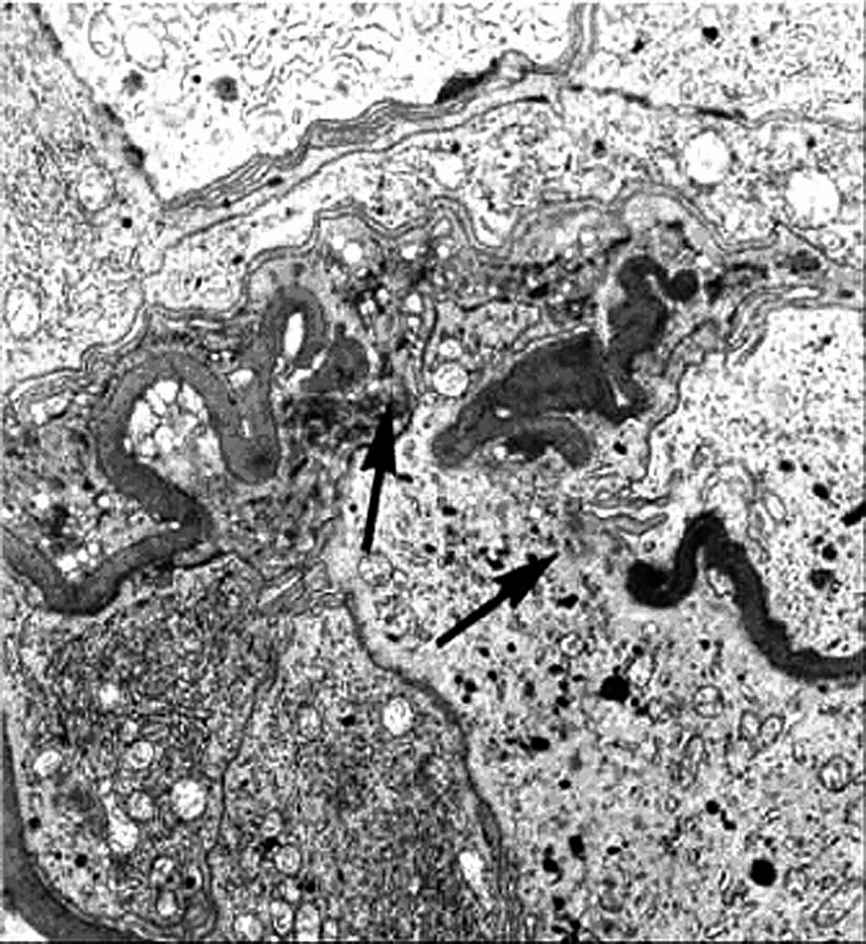
\includegraphics{./images/Image00161.jpg}
 \captionsetup{justification=centering}
 \caption{新月体性肾小球肾炎\\ {\small 电镜下见基膜局灶性缺损和断裂(箭头所示)}}
\label{fig10-14}
  \end{figure}

(4)免疫荧光:见IgG和C3沿毛细血管襻分布,I型为线性荧光,Ⅱ型为颗粒状荧光,Ⅲ型免疫荧光检查结果为阴性。

\paragraph{临床病理联系}
主要表现为快速进行性肾小球肾炎综合征。起病急,进展快,少尿或无尿,明显血尿,伴红细胞管型或中度蛋白尿、高血压、氮质血症和快速进行性肾功能不全。

由于肾小球毛细血管纤维素样坏死、基膜缺损和缺血,故血尿明显,蛋白尿相对较轻。由于大量新月体形成和球囊腔阻塞,肾小球滤过率下降而肾小管重吸收功能尚正常,故病人迅速出现少尿、无尿和氮质血症等症状。高血压主要是由于钠、水潴留,血容量增加,新月体压迫肾缺血激活的肾素-血管紧张素系统有协同作用。病变后期肾小球玻璃样变,肾单位功能丧失,最终发生肾衰竭。

\paragraph{预后}
新月性肾小球肾炎预后较差,尽管通过适当的血液透析后症状可显著减轻,但大多数病人最终还是发展为慢性肾衰竭。病人的预后一般与呈现新月体的肾小球的比例相关,新月体性肾小球少于75%者病程稍长,超过80%者多在半年内死于尿毒症。

\subsubsection{肾病综合征及相关的肾炎类型}

肾病综合征最重要的特征是肾小球毛细血管壁损伤,使血浆蛋白滤过增加,形成大量蛋白尿。若滤过膜的损伤相对较轻,滤过的为低分子量的清蛋白和转铁蛋白,则为选择性蛋白尿,相反,损伤严重时大分子量的蛋白也可滤过,则形成非选择性蛋白尿。若长期大量蛋白尿使血浆蛋白丢失过多,则形成低蛋白血症,血浆胶体渗透压降低,大量水分外漏引起组织高度水肿,同时血容量下降,使肾小球滤过减少,醛固酮和抗利尿激素分泌增加,致使钠、水潴留,水肿加重。低蛋白血症还可刺激肝脏合成脂蛋白,引起高脂血症。肾小球基膜通透性增高,脂蛋白滤过增加则可引起脂质尿。

多种原发性肾小球肾炎和系统性疾病均可引起肾病综合征。年龄与肾病综合征的发生有关,其中儿童主要由原发性肾小球病引起,成人中系统性疾病的比例增高。常见的病因见表\ref{tab10-2}。本部分介绍几种能引起肾病综合征的原发性肾小球病。

\begin{longtable}[htbp]{lll}
    \caption{肾病综合征的原因}
    \label{tab10-2}\\
    \toprule
    原因 &儿童患病率(\%) &成人患病率(\%)\footnote{引自Robbins Basic
Pathology(第9版)。儿童的肾病综合征中约有95%由原发性肾小球病引起,系统性疾病仅约5%;成人的肾病综合征中原发性肾小球病约占60%,系统性疾病占40%。}\\
    \midrule
    原发性肾小球病&&\\
膜性肾小球病&5&30\\
微小病变性肾小球病&10&35\\
局灶性节段性肾小球硬化&10&10\\
膜增殖性肾小球肾炎&10&10\\
IgA肾病及其他&10&15\\
伴肾病表现的系统性疾病&&\\
糖尿病&&\\
淀粉样变性&&\\
系统性红斑狼疮&&\\
某些药物(金,青霉胺,海洛因)&&\\
传染病(疟疾,梅毒,乙肝,艾滋病)&&\\
恶性肿瘤(癌.黑色素瘤)&&\\
其他(蜂叮咬,遗传性肾炎)&&\\
    \bottomrule
\end{longtable}

\paragraph{膜性肾小球病(膜性肾病)}
膜性肾小球病(membranous
glomerulopathy),或称膜性肾小球肾炎,因病变早期光镜下肾小球炎症不明显,所以又称膜性肾病(membranous
nephropathy)。为缓慢进展性疾病,常见于30~50岁,在我国是引起成人肾病综合征最常见的原因,特征为含有免疫球蛋白的电子致密物沉积于肾小球基膜的上皮下,使毛细血管壁弥漫性增厚。

(1)病因和发病机制:膜性肾小球病是慢性免疫复合物性肾炎的一种类型,约有85%为原发性,其余为继发性。原发性膜性肾小球病被认为是与Heymann肾炎相似的与易感基因有关的自身免疫病。自身抗体与肾小球上皮细胞膜抗原反应,在上皮细胞和基膜之间形成免疫复合物。病变部位通常没有中性粒细胞、单核细胞浸润和血小板沉积,但有补体出现,由补体C5b-C9组成的膜攻击复合体可激活肾小球上皮细胞和系膜细胞,释放蛋白酶和氧化剂,引起毛细血管壁损伤和蛋白漏出。

(2)病理变化:肉眼见双肾肿大,色苍白,有“大白肾”之称。晚期体积缩小,表面呈颗粒状。光镜下早期肾小球基本正常,之后肾小球毛细血管壁均匀一致的弥漫性增厚(图\ref{fig10-15}A)。若用PASM染色可显示黑色的基膜上有钉突状突起(图\ref{fig10-15}B)。后期,极度增厚的基膜使毛细血管腔受压狭窄或闭塞,肾小球缺血,最终导致肾小球纤维化和玻变。近曲小管上皮细胞肿胀,内常含有玻璃样小滴及脂肪空泡,为被吸收的蛋白小滴。肾间质有慢性炎细胞浸润和纤维化。电镜显示上皮细胞肿胀,足突消失,上皮与基膜之间有大量电子致密沉积物,呈钉突或圆顶状。早期,沉积物之间基膜样物质增多,形成钉状突起与增厚的基膜垂直,形如梳齿。之后,钉突向沉积物表面延伸并将其覆盖,使基膜明显增厚。晚期,被包裹的沉积物逐渐被溶解吸收,形成“虫蚀状”空隙(图\ref{fig10-16})。最后,基膜上的空隙被基膜样物质所填充,基膜显著增厚,毛细血管腔受压狭窄或闭塞,肾小球缺血,最终导致肾小球纤维化和玻变。免疫荧光显示免疫球蛋白IgG和补体C3沉积,沿基膜呈弥漫性的颗粒状分布(图\ref{fig10-17})。病变后期无免疫球蛋白或仅有少量C3沉积。

\begin{figure}[!htbp]
 \centering
 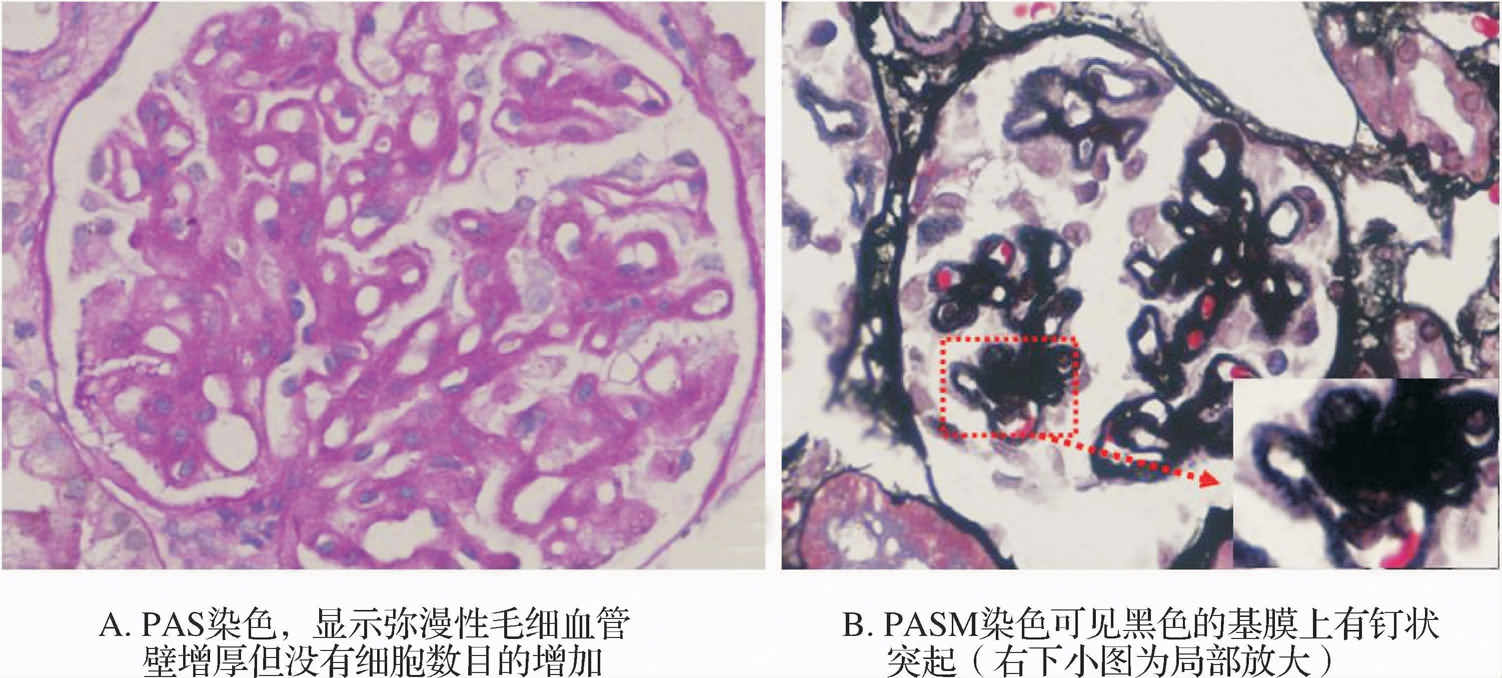
\includegraphics{./images/Image00163.jpg}
 \captionsetup{justification=centering}
 \caption{膜性肾小球病(高倍)}
 \label{fig10-15}
  \end{figure} 

\begin{figure}[!htbp]
 \centering
 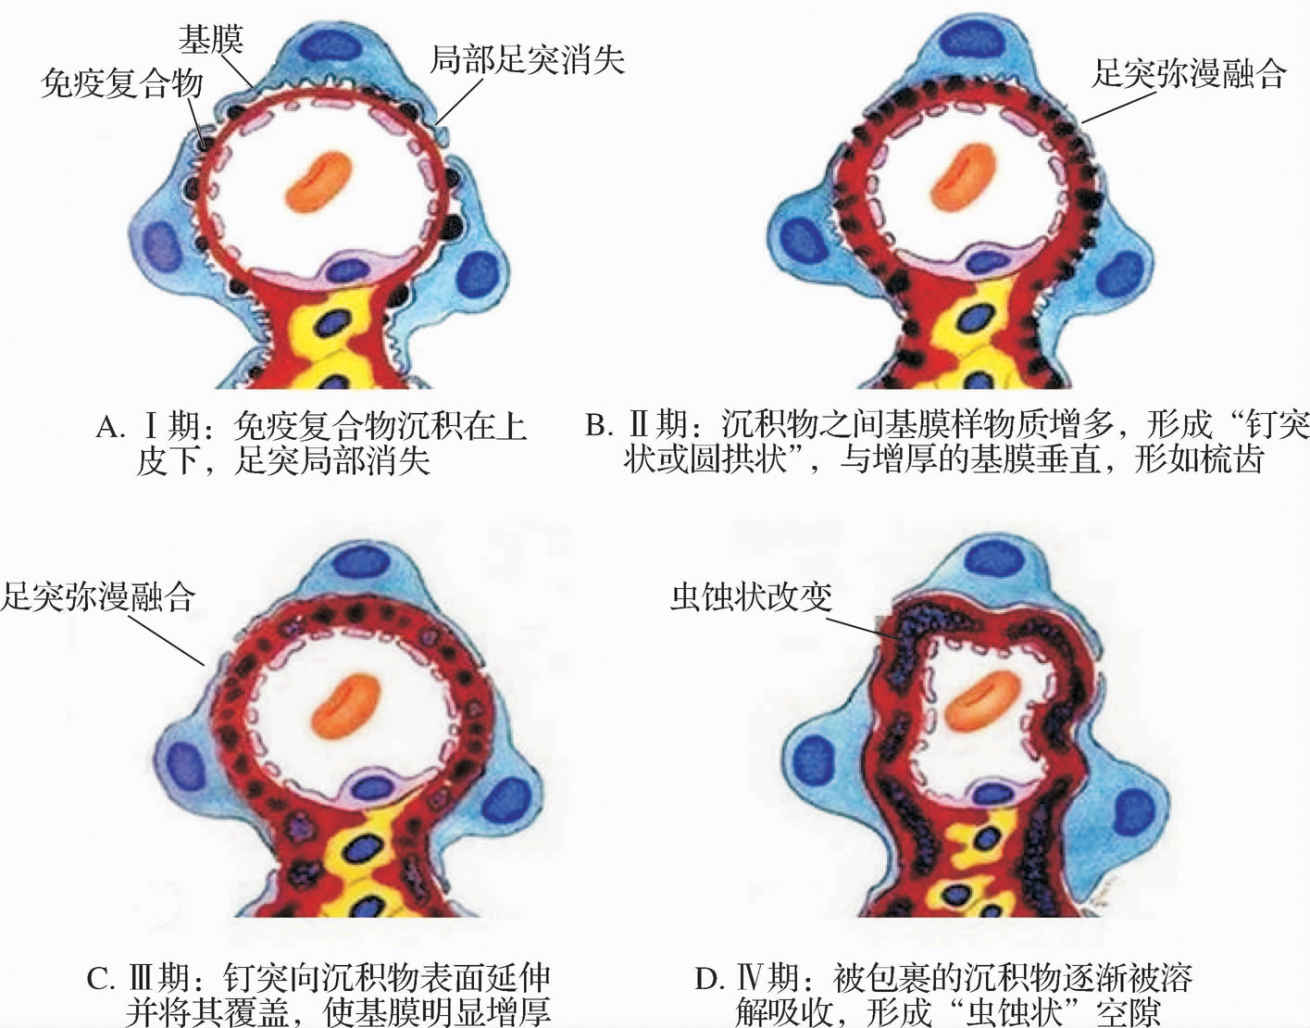
\includegraphics{./images/Image00164.jpg}
 \captionsetup{justification=centering}
 \caption{膜性肾小球病发展阶段模式图}
 \label{fig10-16}
  \end{figure} 

\begin{figure}[!htbp]
 \centering
 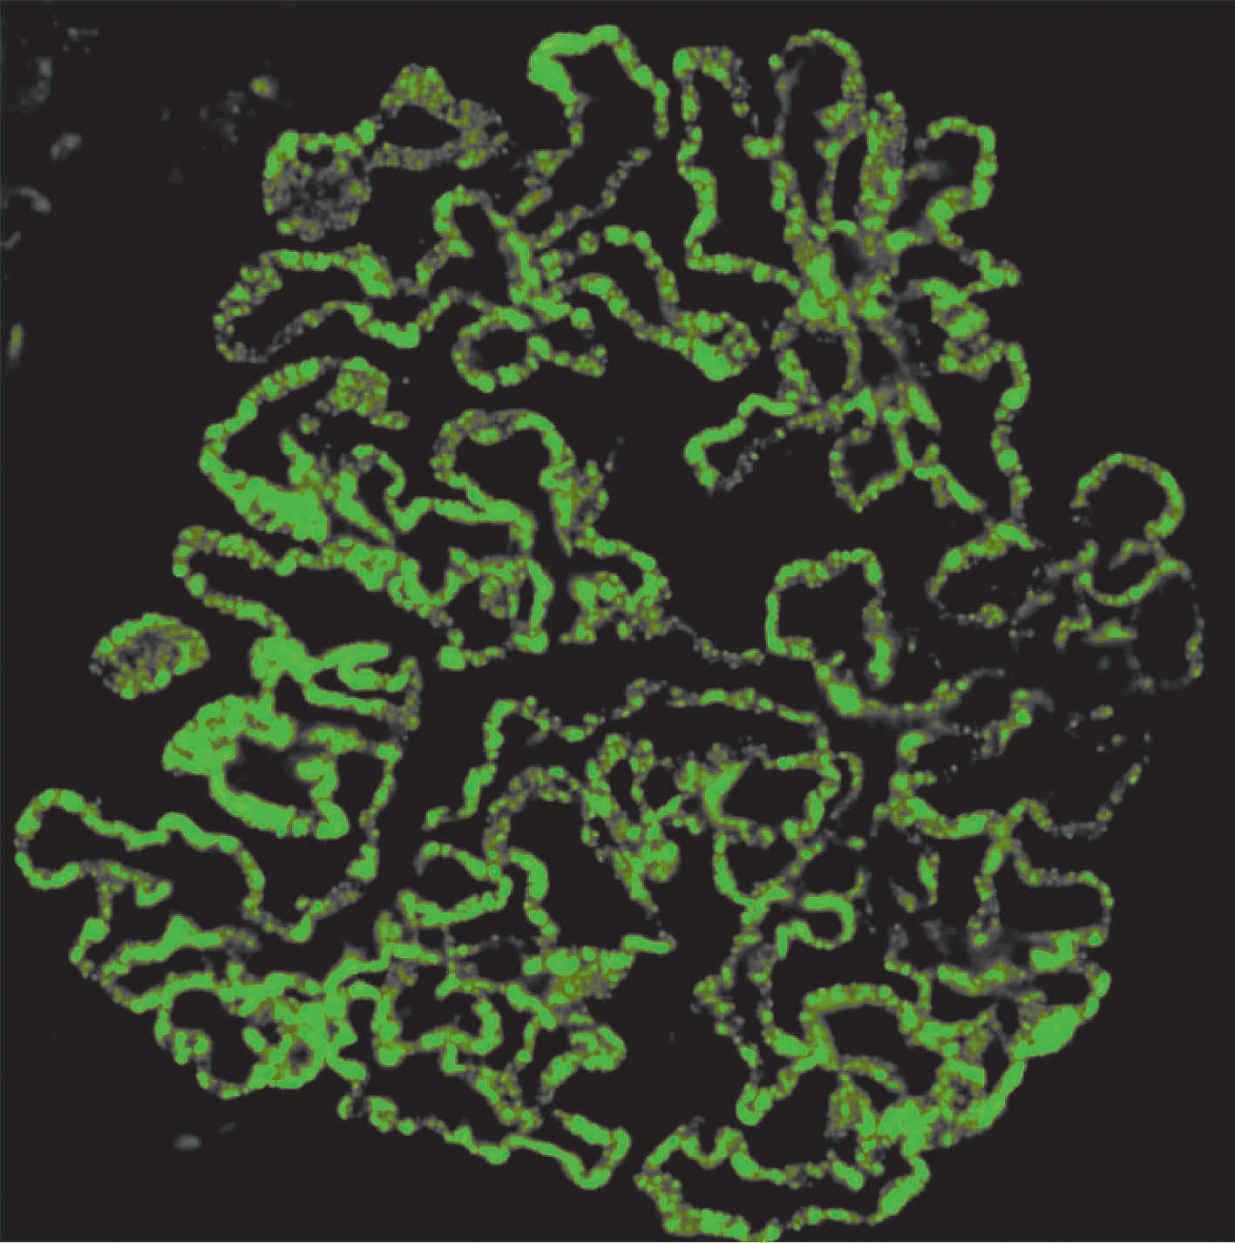
\includegraphics{./images/Image00165.jpg}
 \captionsetup{justification=centering}
 \caption{膜性肾小球病\\ {\small IgG免疫荧光沿肾小球毛细血管基膜分布,呈颗粒状}}
\label{fig10-17}
  \end{figure}

(3)临床病理联系:本型多见于成人,起病隐匿,主要表现为肾病综合征,或呈低于肾病范围的蛋白尿(约占15%)。由于肾小球基膜严重损伤,滤过膜通透性增高显著,常表现为非选择性蛋白尿。部分病人伴有血尿或轻度高血压。

任何患有膜性肾小球肾炎的病人必须首先排除上述的各种继发性疾病。随着肾小球硬化的进展,肾功能日趋丧失,并在晚期出现尿毒症,表现为终末期慢性肾小球肾炎的症状。

(4)预后:膜性肾小球病对类固醇类药物治疗不敏感,病程多呈慢性进行性,约一半原发性病例经过2~20年时间进展为慢性肾衰竭,仅10%~30%的病人可部分或全部缓解,10年内死亡率低于10%。

\paragraph{微小病变性肾小球病(脂性肾病或足突病)}
微小病变性肾小球病(minimal change
glomerulopathy)又称微小病变性肾小球肾炎或微小病变性肾病,是引起儿童(通常为2至6岁)肾病综合征最主要的原因。病变特征为光镜下肾小球基本正常,但在电镜下可见到均匀弥漫性的脏层上皮细胞足突消失,上皮足突的变平和融合是最显著的变化。肾近曲小管上皮内可显示有玻璃样小滴(蛋白尿的证据)和脂质小滴(脂尿的证据),故曾名“脂性肾病”。本病相对良性,临床最显著的特征是对皮质类固醇治疗有显著的疗效。

(1)病因和发病机制:脂性肾病的病因和发病机制不明,由于肾小球内无免疫复合物沉积,一般认为是非免疫复合物或抗肾小球基膜抗体引起的,目前多认为与T细胞免疫功能异常有关。可能是T淋巴细胞和巨噬细胞分泌的细胞因子损伤了脏层上皮细胞,引起滤过膜阴离子丧失的结果。最近有研究显示编码肾素等肾小球蛋白基因的突变与本病有关。

(2)病理变化:肉眼可见肾体积稍肿大,颜色苍白。切面肾皮质见黄白色条纹,是因肾小管上皮细胞吸收脂质并沉积引起。光镜可见:肾小球结构基本正常,部分病例有轻微的系膜增生和基质增多(图\ref{fig10-18}A)。肾近曲小管上皮细胞内出现大量脂质空泡和玻璃样蛋白小滴。电镜可见肾小球基膜基本正常,无沉积物,主要改变是弥漫性脏层上皮细胞足突融合或消失(图\ref{fig10-18}B,C),上皮细胞胞质内常有空泡形成,细胞表面微绒毛增多。值得注意的是膜性肾小球病和糖尿病等疾病也显示有足突消失,所以只有在光镜下肾小球结构正常,脏层上皮细胞足突消失才具有诊断价值。经肾上腺皮质激素治疗后,足细胞的改变可恢复正常。免疫荧光检查显示无免疫沉积物。

\begin{figure}[!htbp]
 \centering
 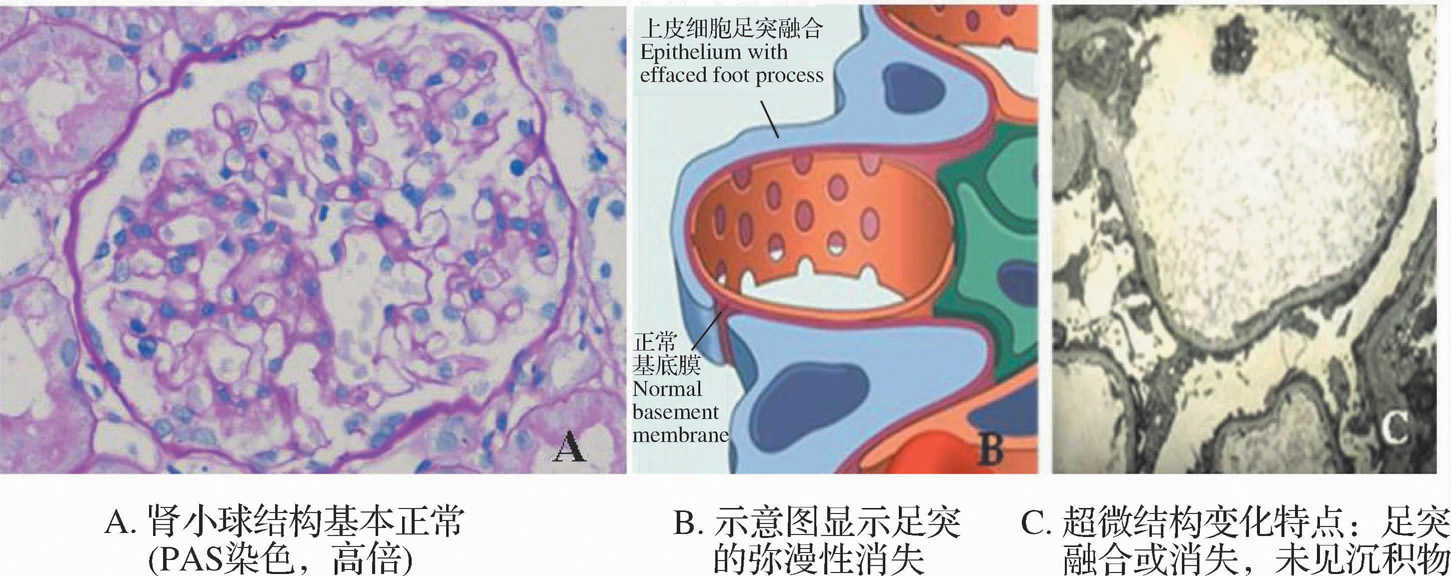
\includegraphics{./images/Image00166.jpg}
 \captionsetup{justification=centering}
 \caption{微小病变性肾小球病}
 \label{fig10-18}
  \end{figure} 

(3)临床病理联系:本病多见于儿童。可发生于呼吸道感染或免疫接种之后。临床主要表现为肾病综合征。水肿常为最早出现的症状。蛋白尿通常为选择性的,成分为小分子的血清蛋白,主要是白蛋白,机制可能是因为T细胞免疫功能异常损伤了脏层上皮细胞,使肾小球多聚阴离子(负性电荷)的丧失,毛细血管壁呈选择性通透性增高。

(4)预后:本病相对良性,90%以上的患儿对短期皮质类固醇治疗敏感,即使部分病人会伴有类固醇激素的依赖,但远期的预后较好。成人患者对激素治疗反应缓慢,疗效较差。不到5%的患者在25年后可以发展为慢性肾衰竭。

\paragraph{局灶性节段性肾小球硬化}
局灶性节段性肾小球硬化(focal segmental
glomerulosclerosis,FSGS)可引起肾病综合征或严重的蛋白尿,病变特点是部分肾小球硬化(局灶性的),以及在受累的肾小球中仅有部分毛细血管襻受到影响(节段性的)。

(1)病因和发病机制:本病具体的病因和发病机制尚不清楚,主要是由脏层上皮细胞的损伤和改变引起。可能由于一些循环因子引起局部通透性明显增高,血浆蛋白和脂质在细胞外基质内沉积,激活系膜细胞而导致。分别见于特发性的、继发性的(继发于另一种形式的肾小球肾炎或慢性肾脏疾病,如IgA肾病、复发性肾病,和伴发性的(伴发于特定的情况,如HIV肾病,海洛因成瘾者肾病)的三种情况。据报道有病人体内存在一种约50kD的非免疫球蛋白性因子,该因子可引起蛋白尿。

(2)病理变化:光镜下病灶呈局灶性,表现为病变的肾小球内部分毛细血管襻系膜基质增加,基膜崩解,玻璃样物质和脂质沉积(图\ref{fig10-19}),早期累及皮髓交界处肾单位,后期可波及皮质全层。偶尔肾小球可以完全硬化伴有肾近曲小管萎缩和间质纤维化,为晚期改变。电镜显示脏层上皮细胞足突消失,部分上皮细胞从肾小球基膜剥脱。免疫荧光为阴性,或在病变部位有IgM和C3沉积。

\begin{figure}[!htbp]
 \centering
 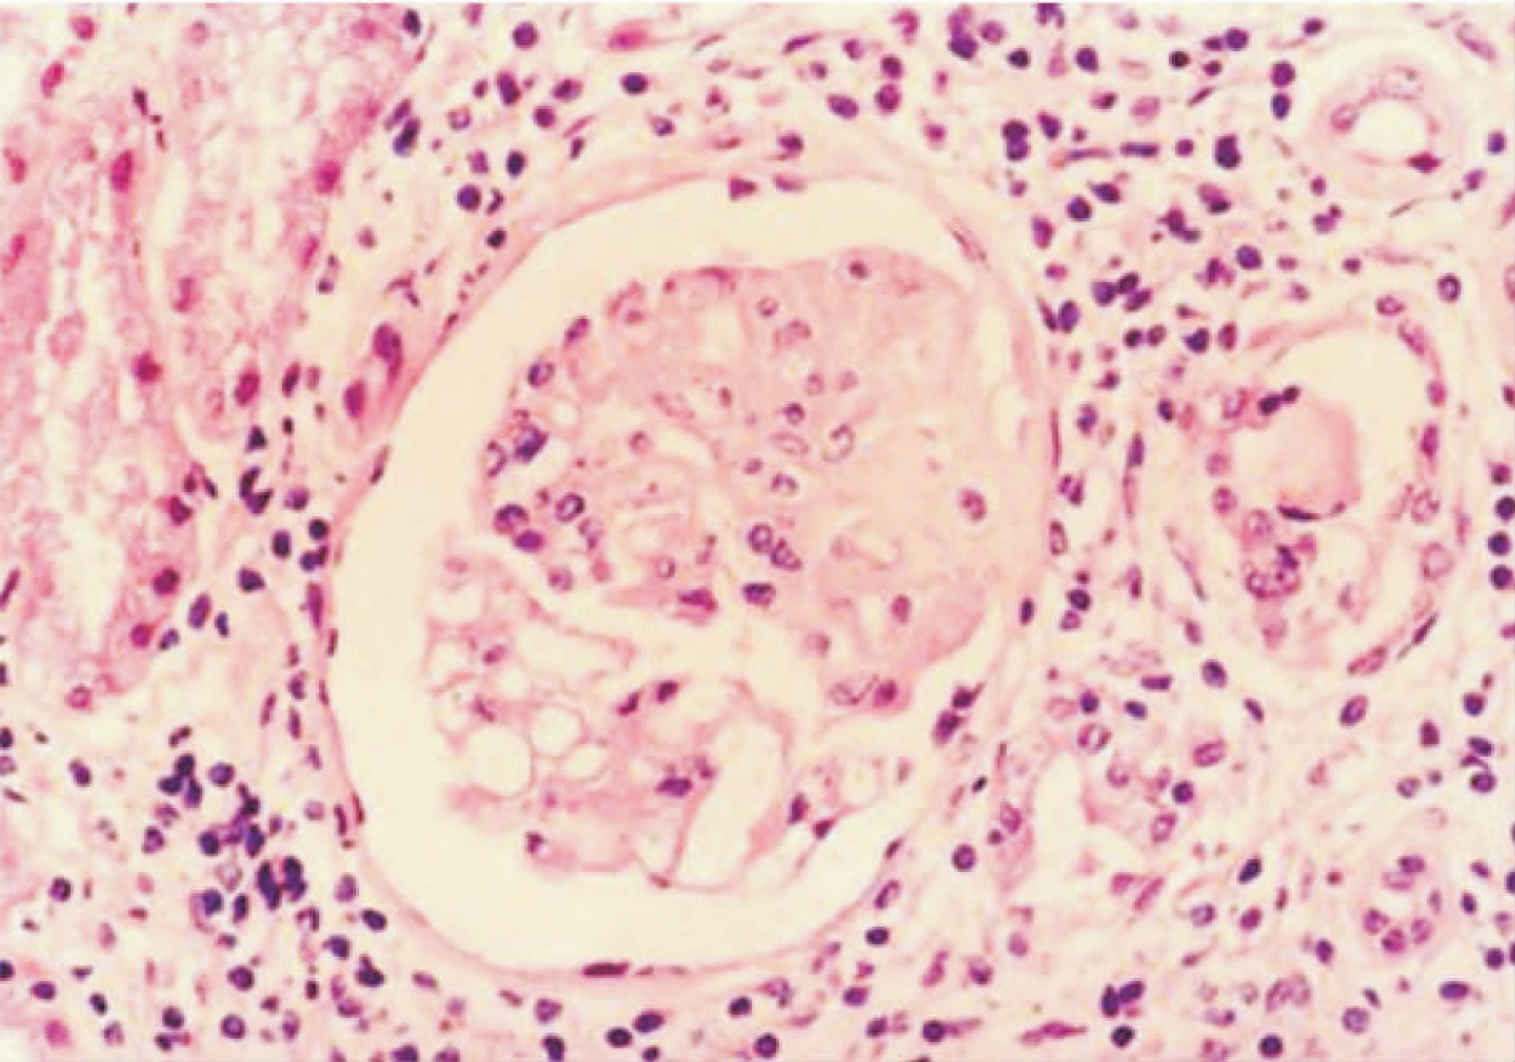
\includegraphics{./images/Image00167.jpg}
 \captionsetup{justification=centering}
 \caption{局灶性节段性肾小球硬化\\ {\small 病变显示肾小球内部分毛细血管襻系膜基质增加,基膜崩解,玻璃样物质和脂质沉积(HE染色,高倍)}}
\label{fig10-19}
  \end{figure}

(3)临床病理联系:大部分病人临床表现为肾病综合征,少数仅表现为蛋白尿。

原发性或特发性局灶性节段性肾小球硬化占肾病综合征的10%,在儿童须与由脂性肾病引起的肾病综合征鉴别,因为临床病理显著不同。局灶性节段性肾小球硬化的以下特点可与轻微病变性肾小球病相区别:①出现血尿,肾小球滤过率下降和高血压的比例较高;②非选择性蛋白尿;③类固醇疗效差或无效;④至少50%的病人10年内发展为慢性肾衰竭;⑤在硬化区域内出现IgM和C3沉积。

(4)预后:本病多发展为慢性肾小球肾炎,50%的病人在发病后十年内发展为终末期肾小球肾炎。小儿患者预后较好。

\paragraph{膜性增生性肾小球肾炎}
膜性增生性肾小球肾炎(membranoproliferative
glomerulonephritis,MPGN)是一种比较严重的组织学类型,临床上大部分病例(2/3)表现为肾病综合征。病变既有毛细血管基膜不规则增厚,又有肾小球系膜细胞增生和系膜基质增多,又称为系膜毛细血管性肾小球肾炎。根据发病机制和电镜下电子致密物沉积部位不同,又可分为Ⅰ型、Ⅱ型和Ⅲ型,Ⅲ型极为少见。

(1)病因和发病机制:本病可以是原发性的,也可以是继发性的。Ⅰ型由循环免疫复合物沉积引起,并有补体的激活。引起免疫反应的抗原成分尚未确定。Ⅱ型显示有激活补体替代途径的证据(血清C3、备解素和B因子减少)。大多数Ⅱ型病人在血清中有C3致肾炎因子,该因子是一种自身抗体,与C3转化酶结合,使之不易被降解,导致补体替代途径持续激活,C3不断分解。由于C3过度消耗和肝脏C3合成减少,病人出现低补体血症。C3致肾炎因子引起肾小球损伤的确切机制和致密沉积物的性质目前还不清楚。

(2)病理变化:光镜下两个类型的病变相似。肾小球体积增大,系膜细胞和内皮细胞数量增多,可有白细胞浸润,肾小球基膜不规则增厚。部分病例有新月体形成。由于系膜细胞增生和系膜基质增多,血管球小叶分隔增宽,呈“叶”状,故又称分叶状肾炎(图\ref{fig10-20}A)。上述变化经用PASM(图\ref{fig10-20}B)和PAS染色特别明显。电镜下肾小球毛细血管壁基膜增厚呈“双轨状”或“履带状”(图\ref{fig10-21}A),后者由系膜细胞、内皮细胞或白细胞突起嵌入延伸插入邻近的毛细血管襻所致,所以称为“系膜插入物”,这也是另一个命名“系膜毛细血管性肾小球肾炎”的由来。Ⅰ型显示有内皮下的电子致密沉积物和少数上皮下和系膜区的C3沉积物(图\ref{fig10-21}B)、早期的补体成分(C1q和C4)以及呈颗粒状沉积的免疫球蛋白。Ⅰ型改变可能发生在伴有SLE、乙型或C型肝炎、房室分流后感染、血吸虫病、α1-抗胰蛋白酶缺乏症、慢性肝病的病人和某些恶性病例。Ⅱ型(致密沉积物病)较少见,显示肾小球基膜内含有带状形式的电子密度极高的沉积物(图\ref{fig10-21}C)。偶尔也会发现上皮下“驼峰状”沉积物,C3也有显示,但没有早期补体成分。

\begin{figure}[!htbp]
 \centering
 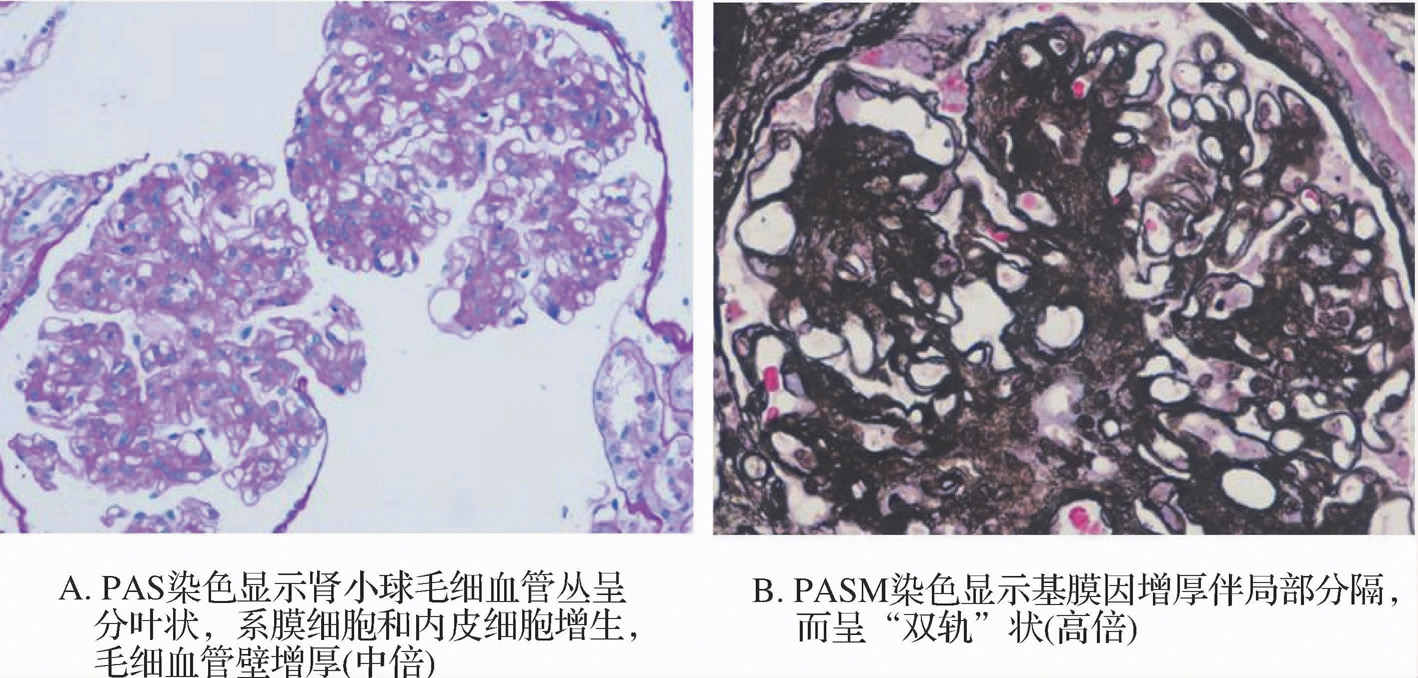
\includegraphics{./images/Image00168.jpg}
 \captionsetup{justification=centering}
 \caption{膜性增生性肾小球肾炎}
 \label{fig10-20}
  \end{figure} 

\begin{figure}[!htbp]
 \centering
 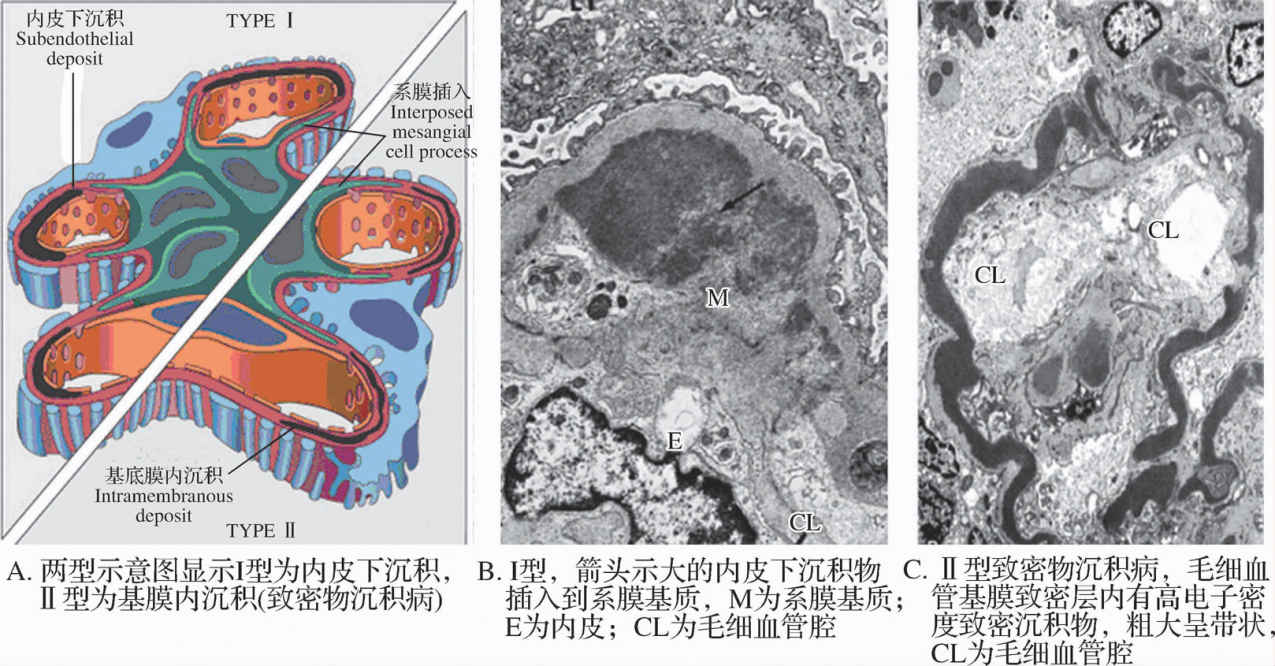
\includegraphics{./images/Image00169.jpg}
 \captionsetup{justification=centering}
 \caption{膜性增生性肾小球肾炎}
 \label{fig10-21}
  \end{figure} 

(3)临床和预后:本病多发生于儿童和青年,主要表现为肾病综合征(占儿童和成人原发性肾病综合征的5%~10%),常伴有血尿,也可仅表现为蛋白尿。病变常为慢性进展性,预后较差。伴有大量新月体形成的病人可出现急进性肾炎的临床表现。尽管类固醇可延缓该病的病程,还是有约50%的病人在10年内发展为慢性肾衰竭。本病在接受肾移植的受体中有很高的复发率,尤其是Ⅱ型疾病患者。

{知识链接}

C3肾小球病是近年提出的新概念,其诊断标准为:肾小球以补体C3沉积为主(C3免疫荧光强度较其他免疫分子荧光强度≥2+)。包括致密沉积物病(dense
deposit disease
DDD)和C3肾小球肾炎;DDD的特征是:在肾小球基膜致密层呈均质飘带样电子致密物的沉积;除DDD以外的其他C3肾小球病基本都被归为C3肾小球肾炎,C3肾小球肾炎的电子致密物可在系膜区、内皮下、上皮下、甚至肾小球基膜内(但与DDD电子致密物的性质不同)沉积,C3肾小球肾炎的光镜表现可多样,如膜性增生性肾小球肾炎、系膜增生性肾小球肾炎、毛细血管内增生性肾炎、轻微病变或光镜表现正常,严重时可伴不同程度的新月体形成。

\paragraph{系膜增生性肾小球肾炎}
系膜增生性肾小球肾炎(mesangioproliferative
glomerulonephritis)的病变特点是弥漫性系膜细胞增生及系膜基质增多。本病在我国和亚太地区常见,在欧美则较少发生。

(1)病因和发病机制:原发性系膜增生性肾小球肾炎的病因和发病机制尚未明确,可能存在多种致病途径,如循环免疫复合物沉积或原位免疫复合物形成等。免疫反应通过介质的作用刺激系膜细胞,导致系膜细胞增生、系膜基质增多。

(2)病理变化:光镜下:主要改变为弥漫性系膜细胞增生和系膜基质增多。电镜下:1/4~1/2病例可在系膜区见到少量稀疏的细颗粒状和云雾状的电子致密物。免疫荧光检查常显示不同的结果,分如下四类:①以IgM为主的免疫球蛋白及C3沉积者;②以IgG为主的免疫球蛋白及C3沉积者;③仅补体C3沉积者(上述免疫球蛋白及补体均呈颗粒状沉积于系膜区,有时也同时沉积于肾小球毛细血管壁);④免疫病理检查阴性者。在我国最常见的是IgG及C3沉积,在其他国家则多表现为IgM和C3沉积(又称IgM肾病)。

(3)临床病理联系:本病多见于青少年,男性多于女性。起病前常有上呼吸道感染等前驱症状。临床表现具有多样性,可表现为肾病综合征,也可表现为无症状蛋白尿(约30%)和(或)血尿(70%~90%,其中多为镜下血尿,约30%病例为反复发作的肉眼血尿)。

(4)预后:本病可用激素和细胞毒药物治疗。病变轻者疗效好,约50%以上的病人用激素治疗后可获得完全缓解,其远期预后目前仍不十分清楚。病变严重者预后多数不好,迟早会出现较严重的局灶性节段性肾小球硬化,甚至出现肾功能障碍与衰竭。

\subsubsection{IgA肾病}

IgA肾病(IgA
nephropathy)常发生于儿童和青年,在全球范围内是最常见的肾炎类型,但在不同地区的发病率差别很大,在亚洲和太平洋地区的发病率很高。据报道在我国的发病率约占原发性肾小球疾病的30%。本病通常表现为反复发作的镜下或肉眼血尿,是引起反复发作的肾小球性血尿最主要的原因。因病变特点是免疫荧光显示系膜区有IgA沉积,故名IgA肾病,又由于本病由Berger于1968年最先描述,又称Berger病。

\paragraph{病因和发病机制}
IgA肾病可为原发、独立的疾病,也可由过敏性紫癜、肝脏和肠道疾病等继发引起。病人血清中聚合IgA增高,或可出现含有IgA的免疫复合物。IgA肾病的发生与某些HLA表型导致的IgA合成、分泌或清除的调节异常有关。资料表明病毒、细菌和食物蛋白等的刺激,可使呼吸道或消化道黏膜IgA合成增多,其中的IgA1或含IgA1的免疫复合物沉积于系膜区,并激活补体替代途径,引起了肾小球损伤。

\paragraph{病理变化}
IgA肾病的组织学改变差异很大。最常见的是系膜增生性病变(图\ref{fig10-22}A),也可表现为局灶性节段性增生或硬化。少数病例可有较多新月体形成。

电镜检查显示系膜区有电子致密沉积物(图\ref{fig10-22}B)。免疫荧光的特征为系膜增生和系膜区IgA沉积(图\ref{fig10-22}C),提示大的循环IgA复合物积聚在系膜区。IgA肾病常伴有C3和备解素,也可出现少量IgG和IgM,通常无补体早期成分。

\begin{figure}[!htbp]
 \centering
 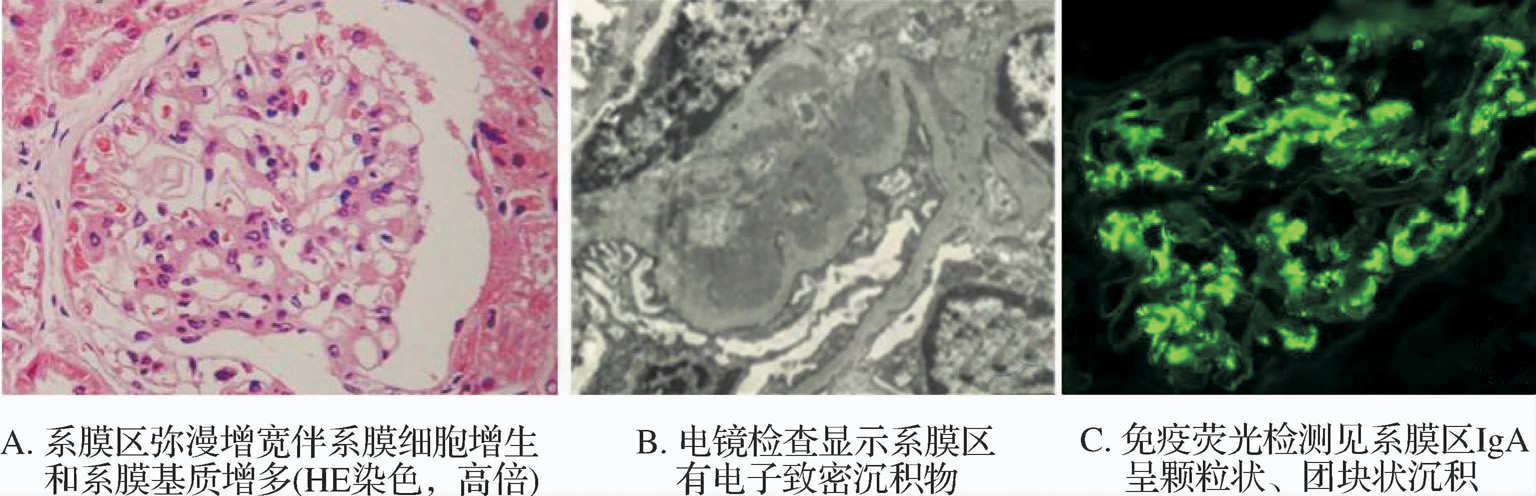
\includegraphics{./images/Image00170.jpg}
 \captionsetup{justification=centering}
 \caption{IgA肾病}
 \label{fig10-22}
  \end{figure} 

\paragraph{临床病理联系}
IgA肾病可发生于不同年龄的个体,儿童和青年多发。发病前常有上呼吸道感染,少数发生于胃肠道或尿路感染后。30%~40%的病人仅出现镜下血尿,可伴有轻度蛋白尿。5%~10%的病人表现为急性肾炎综合征。血尿的典型症状为持续数天而后消退,但每过数月便会复发。

\paragraph{预后}
本病预后差异很大,尽管多数病人病情开始为良性,但15%~40%的病人病情缓慢进展,50%的病人在20年内会发展为慢性肾衰竭。若发病年龄大,严重蛋白尿、高血压、新月体形成和血管硬化则提示预后不佳。肾移植后可重新出现IgA沉积,并引起相应的临床改变。

\subsubsection{慢性肾小球肾炎}

慢性肾小球肾炎(chronic
glomerulonephritis)为许多不同类型肾小球肾炎发展而来的肾小球疾病的终末期共同病变(终末肾),多见于成人,预后差。病变特点是双侧肾小球弥漫性萎缩、玻璃样变和硬化,又称慢性硬化性肾小球肾炎,也称慢性肾炎。

\paragraph{病因和发病机制}
慢性肾小球肾炎由不同类型的肾炎发展形成,这些肾炎类型及进展比例包括:

(1)链球菌感染后肾小球肾炎(儿童1%~2%,成人比例较高);

(2)急进性肾小球肾炎(90%);

(3)膜性肾小球病(50%);

(4)局灶性节段性肾小球硬化(50%~80%);

(5)膜性增生性肾小球肾炎(50%);

(6)系膜增生性肾炎;

(7)IgA肾病(30%~50%);

(8)约20%的病例不清楚由何种肾小球疾病发展而来或缺乏早期肾小球肾炎病史。一是因为慢性肾小球肾炎中的肾小球大多被玻璃样结缔组织所取代,起始的病变类型很难辨认。二是因为有相当数量的慢性肾炎病人发病隐匿,没有明确的急性或其他类型肾炎的病史,发现时已进入慢性阶段。

\paragraph{病理变化}
(1)肉眼观:呈继发性颗粒性固缩肾,表现为双肾体积缩小,质硬,表面呈弥漫性细颗粒状(图\ref{fig10-23}),包膜粘连。切面肾皮质变薄、不规则变窄和瘢痕化并伴有正常结构纹理的消失。皮髓质界限不清,肾盂周围脂肪增多。

\begin{figure}[!htbp]
 \centering
 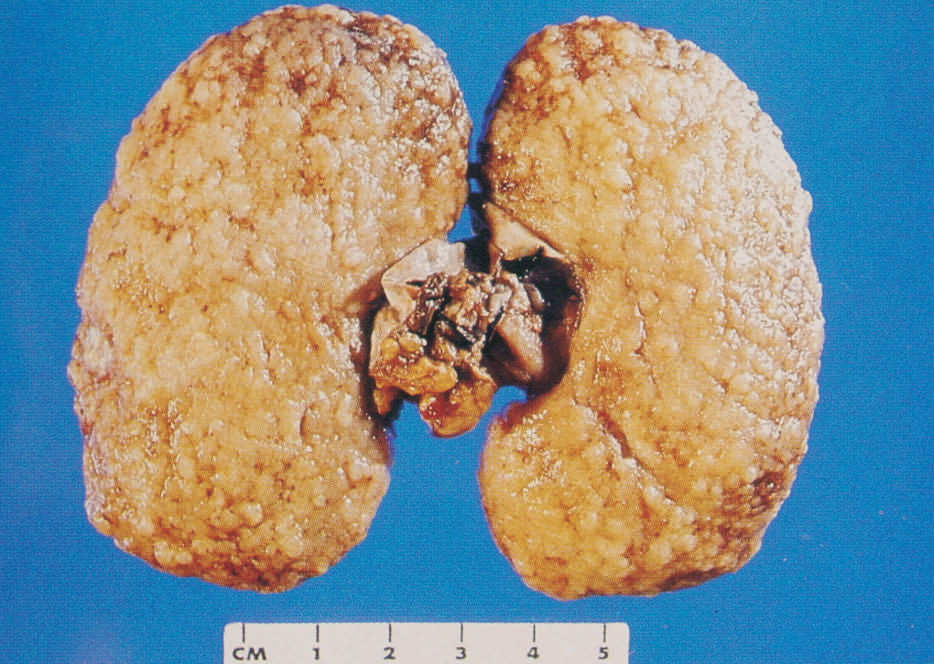
\includegraphics{./images/Image00171.jpg}
 \captionsetup{justification=centering}
 \caption{慢性肾小球肾炎\\ {\small 肾脏对称性缩小,皮质表面呈弥漫颗粒样}}
\label{fig10-23}
  \end{figure}

(2)光镜下:病变早期可能显示有相应类型肾炎的改变,呈现慢性增生性反应,伴有系膜细胞和基质增加(系膜瘢痕化)。之后随病变进展,肾小球内PAS染色阳性的嗜酸性玻璃样物质增多,细胞减少,肾内细、小动脉发生渐发生玻璃样变性和内膜增厚,管腔狭窄。至终末期大量毛细血管闭塞使绝大多数肾小球部分或全部瘢痕化(图\ref{fig10-24})。此时各种类型导致的肾炎病变表现相似,特征表现为病变严重区大部分肾小球(≥75%)发生纤维化和玻璃样变,相应肾小管萎缩消失,代之以间质的纤维化。由于纤维组织的收缩,使玻璃样变性的肾小球相互靠拢,称为肾小球相对集中。病变较轻区肾单位则出现代偿性改变,表现为肾小球体积增大,肾小管扩张,腔内可出现各种管型。肾间质纤维结缔组织明显增生,内见淋巴细胞浸润,有时也见浆细胞和组织细胞。

\begin{figure}[!htbp]
 \centering
 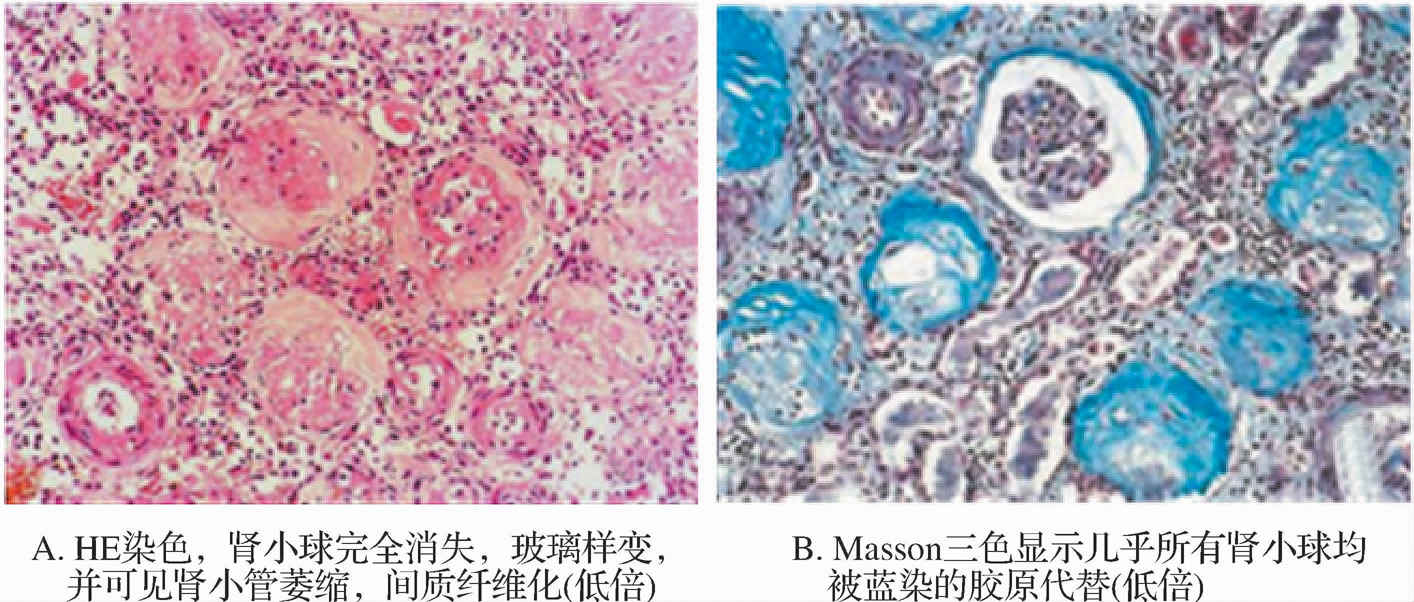
\includegraphics{./images/Image00172.jpg}
 \captionsetup{justification=centering}
 \caption{慢性肾小球肾炎}
 \label{fig10-24}
  \end{figure} 

(3)电镜下:可有毛细血管基膜局灶性增厚,局灶性内皮下沉积物和足突变平。

\paragraph{临床病理联系}
部分病人有其他类型肾炎的病史。部分患者起病隐匿。早期可有食欲差、贫血、呕吐、乏力和疲倦等症状。有的病人则表现为蛋白尿、高血压或氮质血症,亦有表现为水肿者,但由于肾小球闭塞时,蛋白丢失的途径关闭,因此在进展病变中肾病综合征不常见。晚期病人主要症状为慢性肾炎综合征,表现为多尿、夜尿、低比重尿、高血压、贫血、氮质血症和尿毒症。

多尿、夜尿和低比重尿主要由于大量肾单位结构破坏,功能丧失,血液流经残留肾单位时速度加快,肾小球滤过率增加,但肾小管重吸收功能有限,尿浓缩功能降低。尽管可有镜下血尿,但肉眼血尿不常见。

高血压很常见,并可以是主要的临床表现,主要由于肾小球硬化和严重缺血,肾素分泌增多。高血压导致细、小动脉硬化,肾缺血加重,使血压持续增高。长期高血压可导致左心室壁肥厚。

贫血主要由肾单位破坏,促红细胞生成素分泌减少引起。此外,体内代谢产物堆积对骨髓造血功能具有抑制作用。大量肾单位受损使代谢产物不能及时排出,水、电解质和酸碱平衡失调,导致氮质血症和尿毒症。尿毒症患者可出现心外膜炎和胃肠炎等。

\paragraph{预后}
慢性肾小球肾炎病程进展的速度差异很大,但若不治疗的话,预后均很差,残酷地发展为尿毒症,最终多死于因尿毒症或由高血压引起的心力衰竭或脑出血。在首发症状出现到死亡大概是几年或更长些,肾透析和肾移植可以改变这一过程,获得较长期的生存时间。

附:常见原发性肾小球病特点小结(表\ref{tab10-3})。

\begin{table}[htbp]
    \caption{原发性肾小球病特点小结}
    \label{tab10-3}
    \centering
    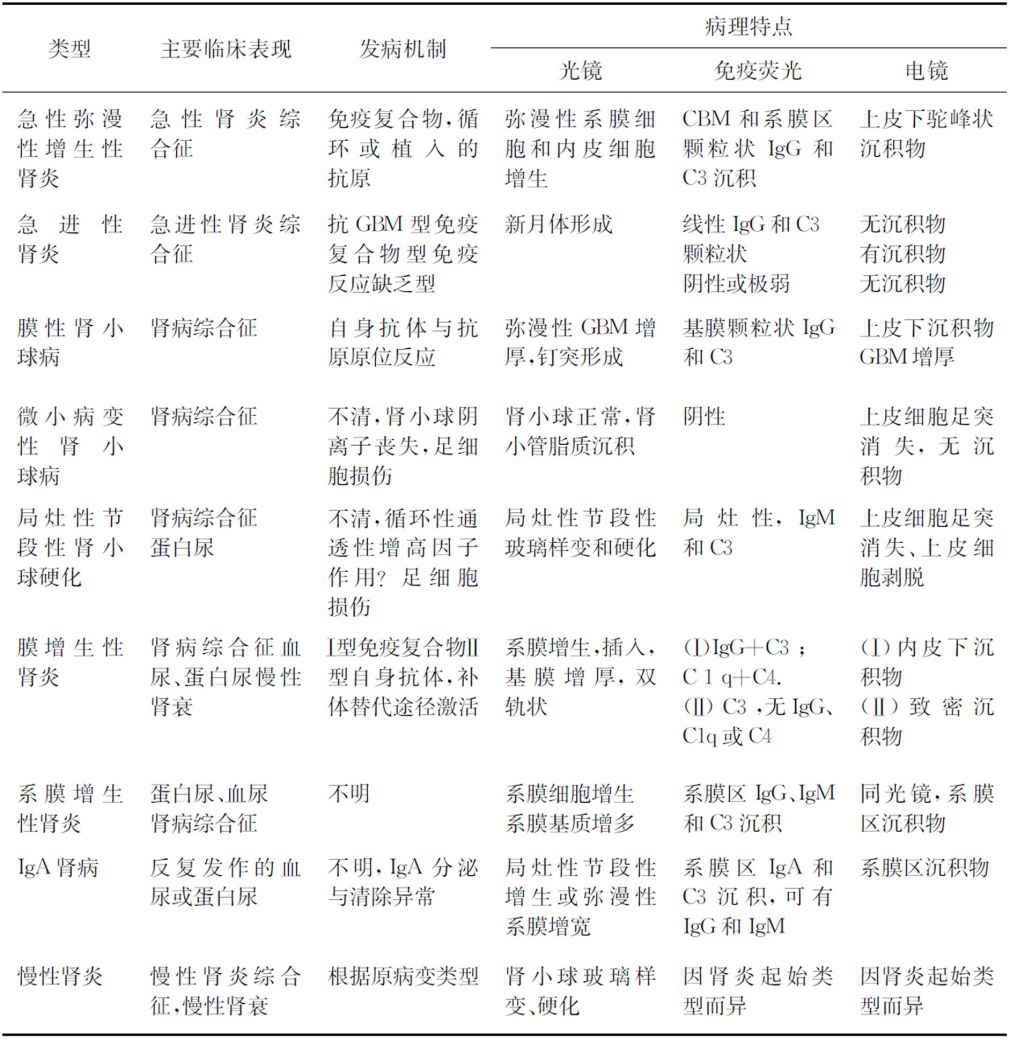
\includegraphics[width=\textwidth]{./images/Image00173.jpg}
\end{table}

\section{肾小管-间质性肾炎}

肾小管-间质性肾炎,又名“间质性肾炎、小管间质性肾病、小管间质性肾炎、间质性肾病”等,为一组累及肾小管和肾间质的炎性疾病,分为急性和慢性两大类,可为由细菌等生物病原体感染和药物、重金属等中毒引起的原发性损伤,也可为肾小球病变、血管性病变、多囊肾和代谢性疾病进展的结果。

肾小管-间质性肾炎的病变主要在髓质,可呈局灶性或弥漫性损害。急性肾小管-间质性肾炎主要表现为间质水肿、间质和肾小管内中性粒细胞等炎细胞浸润,常伴有局灶性肾小管坏死。慢性间质性肾炎表现为淋巴细胞、单核细胞浸润,肾间质纤维化和肾小管萎缩。

本节主要讨论肾盂肾炎和药物引起的肾小管-间质性肾炎。

\subsection{肾盂肾炎}

肾盂肾炎(pyelonephritis)是指肾实质和肾小管都通过间质感染而引起的炎症,以间质的化脓性炎症为特征,包括急性和慢性两种。

\subsubsection{病因和发病机制}

肾盂肾炎多由细菌感染引起,致病菌以肠道革兰阴性菌最常见,其中多数为大肠埃希菌(占60%~80%),其他有变形杆菌、副大肠埃希菌、肠球菌、粪链球菌、葡萄球菌等,还可由霉菌引起。急性肾盂肾炎通常为一种细菌感染引起,慢性肾盂肾炎则可能为多种细菌的混合感染。但由于正常尿液具有自净作用,所以只有在机体全身抵抗力下降或泌尿道局部防御机制被破坏时,致病菌才可能经血源性或上行性感染引起病变。

感染途径及相应的病因有:

(1)血源性传播:亦称下行性感染,多为双侧性,通常在败血症基础上由葡萄球菌或大肠埃希菌引起。

(2)上行性感染:单侧或双侧性,通常由大肠埃希菌、变形杆菌或其他细菌等,引起下尿路感染时,细菌通过尿道、膀胱、膀胱输尿管反流进入肾实质,最终形成肾内反流,或经输尿管周围的淋巴管上行到肾盂、肾盏和肾实质。

易感因素有:①尿路堵塞;②使用器械不当(尤其是操作导管插入时);③膀胱输尿管反流(经结构错乱的膀胱输尿管结合处);④妊娠;⑤先天性异常;⑥糖尿病;⑦免疫抑制;⑧前列腺增生、结石和肿瘤等。

由于女性尿道短、尿道口靠近肛门,容易遭受感染,加上尿道括约肌作用弱,女性激素水平的变化有利于细菌对尿道黏膜的黏附以及性交时黏膜容易受伤等,所以肾盂肾炎在女性非常常见,尤其在15~40岁年龄组,女性与男性发病比率为8∶1。

\subsubsection{急性肾盂肾炎}

急性肾盂肾炎(acute
pyelonephritis)是肾盂、肾间质和肾小管常见的化脓性炎症,主要由细菌感染引起(特别是大肠埃希菌),偶可由多瘤病毒等病毒引起。尿道感染是主要的表现,包括下尿道感染(膀胱炎、前列腺炎、尿道炎)或上尿道肾盂肾炎或同时上、下尿道感染。病变特征为不均匀的、间质性的、化脓性炎症。

\paragraph{病理变化}
(1)肉眼观:肾体积增大,表面充血,表面可见稀疏的黄白色脓肿(图\ref{fig10-25}A),周围见紫红色充血带。病灶局限或弥漫分布,相互融合可形成大脓肿。切面沿髓放线见黄色条纹,向皮质延伸。肾盂黏膜充血水肿,表面有脓性渗出物。严重时,肾盂内有积脓。

(2)镜下:特征为灶性间质性化脓性炎或脓肿形成、肾小管坏死和白细胞管型(图\ref{fig10-25}B)。上行性感染首先累及肾盂,随后波及肾小管;血源性感染常先累及肾皮质,发生于肾小球及其周围的间质,再扩展破坏邻近组织,并向肾盂蔓延。

\begin{figure}[!htbp]
 \centering
 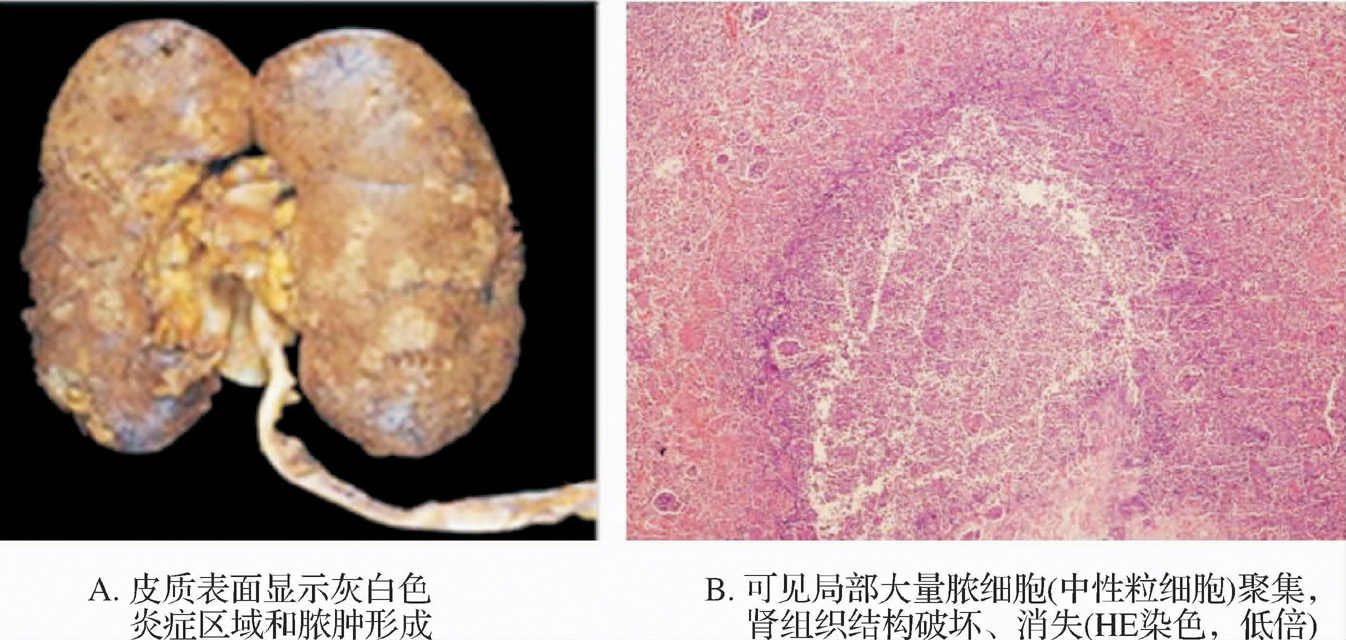
\includegraphics{./images/Image00174.jpg}
 \captionsetup{justification=centering}
 \caption{急性肾盂肾炎}
 \label{fig10-25}
  \end{figure} 

\paragraph{临床病理联系}
通常起病突然,出现发热、寒战、白细胞增多等全身症状,以及尿液的改变,如脓尿、菌尿、血尿、管型尿和蛋白尿等。通常有膀胱和尿路刺激症状如排尿困难、尿频、尿急和尿痛。肾肿大和肾包膜炎病人常伴有肋腰部的疼痛。尿液培养可发现细菌。白细胞管型有临床诊断意义。由于急性肾盂肾炎病变多呈灶状分布,肾小球通常较少受累,一般不出现高血压、氮质血症和肾功能障碍。伴有尿路阻塞、糖尿病或免疫障碍病人的病情常较严重,可发生败血症。并发肾乳头坏死时可发生急性肾衰竭。

\paragraph{预后}
急性肾盂肾炎使用抗生素治疗疗效好。即使本病不治疗其经过也是良性和自限性的,症状往往持续不超过一周,但菌尿可以存在较长时间,若引起感染的诱因未去除或治疗不彻底不确当,则病变易反复发作慢性化,最终使肾组织瘢痕形成并伴有皮质及其下的肾盂肾盏的纤维化变形(上行性感染者易发生)。

常见并发症有:

(1)肾乳头坏死(papillary
necrosis):病变特征是肾锥体乳头侧2/3区域内出现境界清楚的灰白或灰黄色梗死样坏死灶(图\ref{fig10-26})。病变累及单个或所有肾乳头。显微镜下肾乳头发生梗死样的凝固性坏死,正常组织和坏死组织交界处可见中性粒细胞浸润。肾乳头坏死尤其见于糖尿病和尿路堵塞的病例。

\begin{figure}[!htbp]
 \centering
 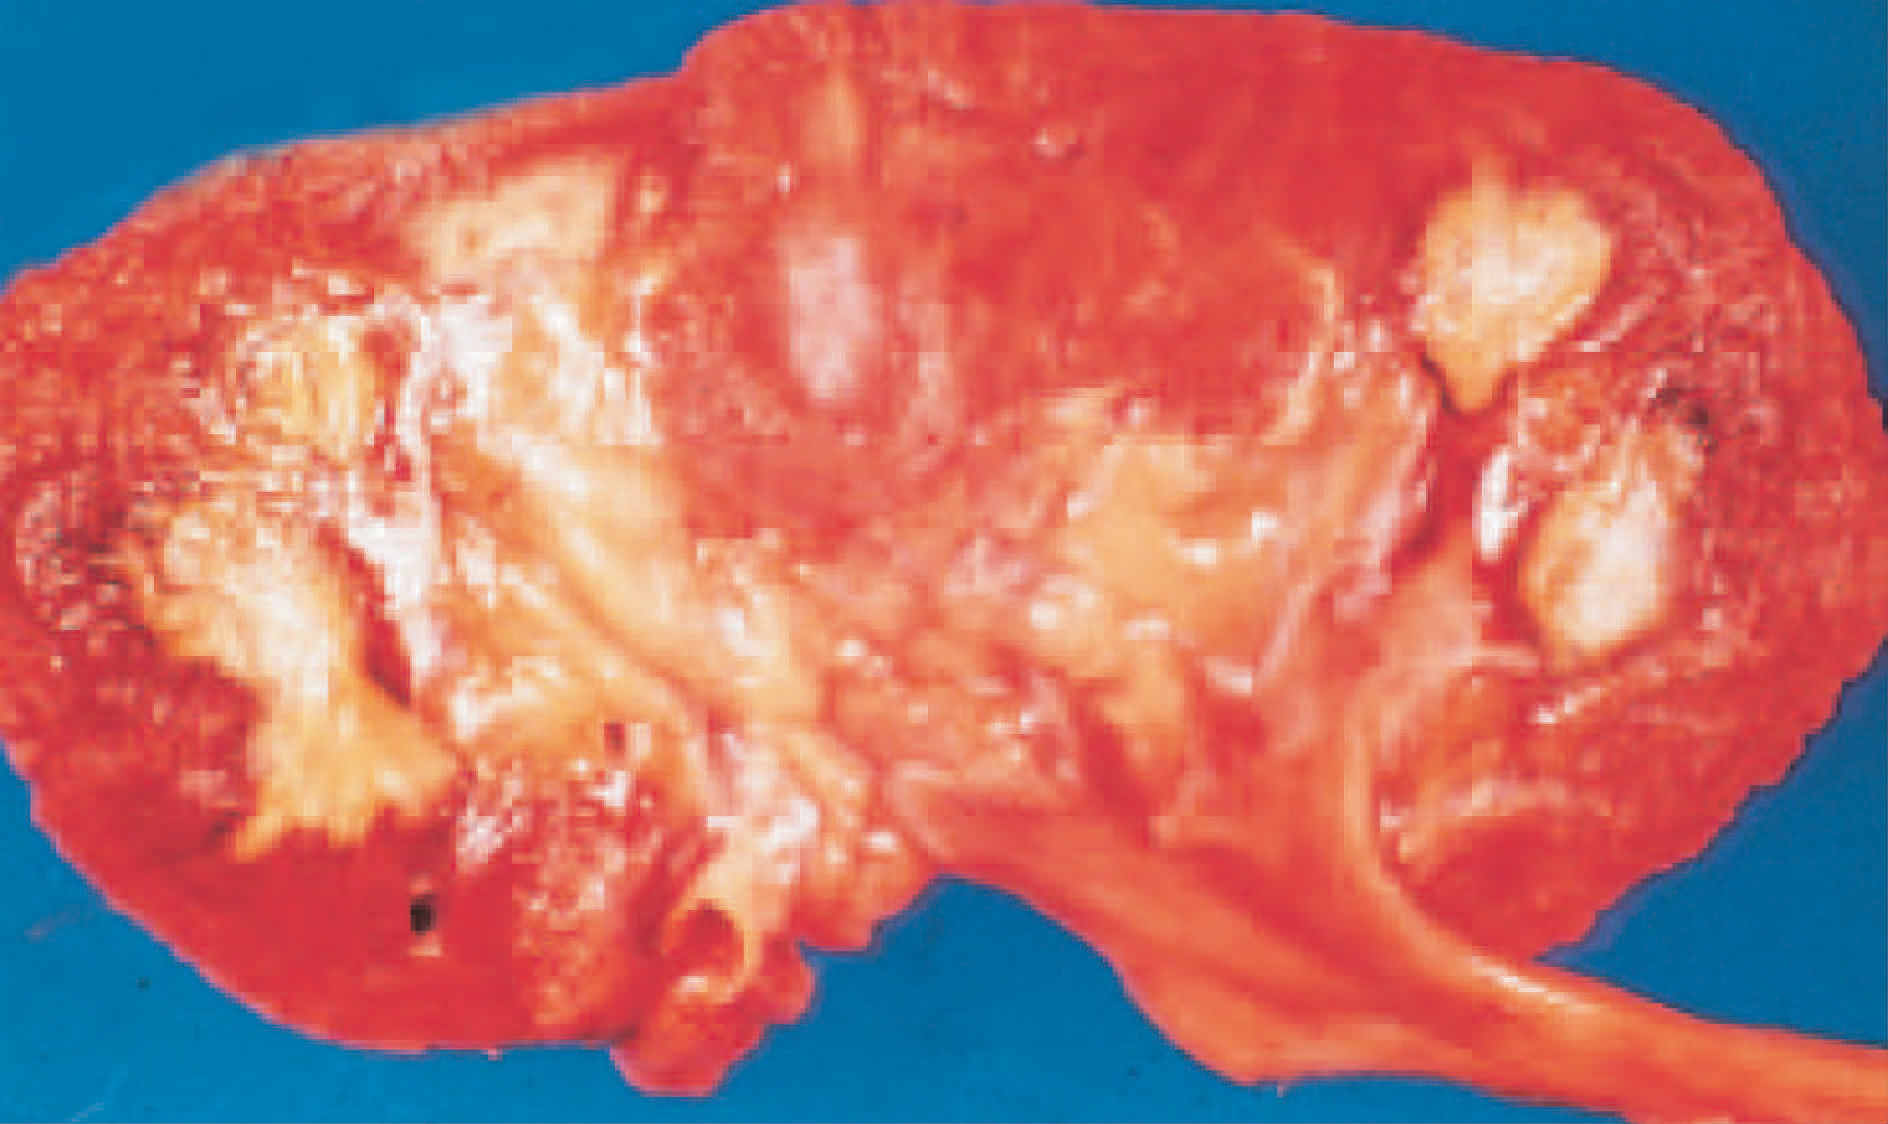
\includegraphics{./images/Image00175.jpg}
 \captionsetup{justification=centering}
 \caption{肾乳头坏死\\ {\small 灰白色的坏死区指向肾乳头}}
\label{fig10-26}
  \end{figure}

(2)肾盂积脓(pyonephrosis):严重尿路阻塞,特别是上尿路的阻塞,脓性渗出不能排除,发生滞留在肾盂、肾盏内形成积脓。

(3)肾周围脓肿(perinephric
abscess):病变严重时肾内化脓性改变可穿破肾被膜,在肾周组织形成脓肿。

\subsubsection{慢性肾盂肾炎}

慢性肾盂肾炎(chronic
pyelonephritis)为肾小管-间质的慢性炎症,伴皮、髓质肾实质瘢痕形成,以及明显的肾盂和肾盏扩张、变平和变形。可由急性肾盂肾炎发展而来,或开始即为慢性。病变呈反复发作性,按原因分有两种类型,分别如下:

(1)慢性阻塞性肾盂肾炎:长期尿路堵塞使肾易于感染,反复多次感染可产生慢性肾盂肾炎。通常由肠道细菌引起,可因阻塞部位的不同而分别呈双侧或单侧性。

(2)伴有反流性肾病:又称为慢性反流性肾盂肾炎,这是慢性肾盂肾炎最常见的原因。起始于儿童,是由于先天性膀胱输尿管反流或肾内反流,可以是单侧或双侧,引起的感染导致慢性肾盂肾炎。反流性肾病起病隐匿,常伴有高血压和多尿症。

\paragraph{病理变化}
(1)肉眼观:一侧或双侧肾脏体积缩小,出现不规则的瘢痕,双侧不对称性(图\ref{fig10-27}
A)。瘢痕多少不等,分布不匀,多见于肾的上、下极。切面见皮髓质界限不清,肾乳头萎缩,肾盏和肾盂因瘢痕收缩而变形,肾盂黏膜粗糙。

(2)镜下:早期肾小球很少受累,主要是局灶性的淋巴细胞、浆细胞浸润和间质纤维化。肾盂黏膜粗糙,在上皮下可见淋巴细胞团。严重的间质炎症可引起肾小管的逐渐萎缩和破坏,甚至导致肾小球玻璃样变。代偿扩张的肾小管内可充满胶样管型类似甲状腺组织形态(甲状腺化)(图\ref{fig10-27}B)。最终,导致形成粗糙U形瘢痕,肾脏体积极度缩小,功能丧失。慢性肾盂肾炎通常是双侧性病变,但两侧肾脏的损害和固缩并不一致。其终末期表现在临床上可与慢性肾小球肾炎混淆。慢性肾盂肾炎急性发作时出现大量中性粒细胞,并有小脓肿形成。

\begin{figure}[!htbp]
 \centering
 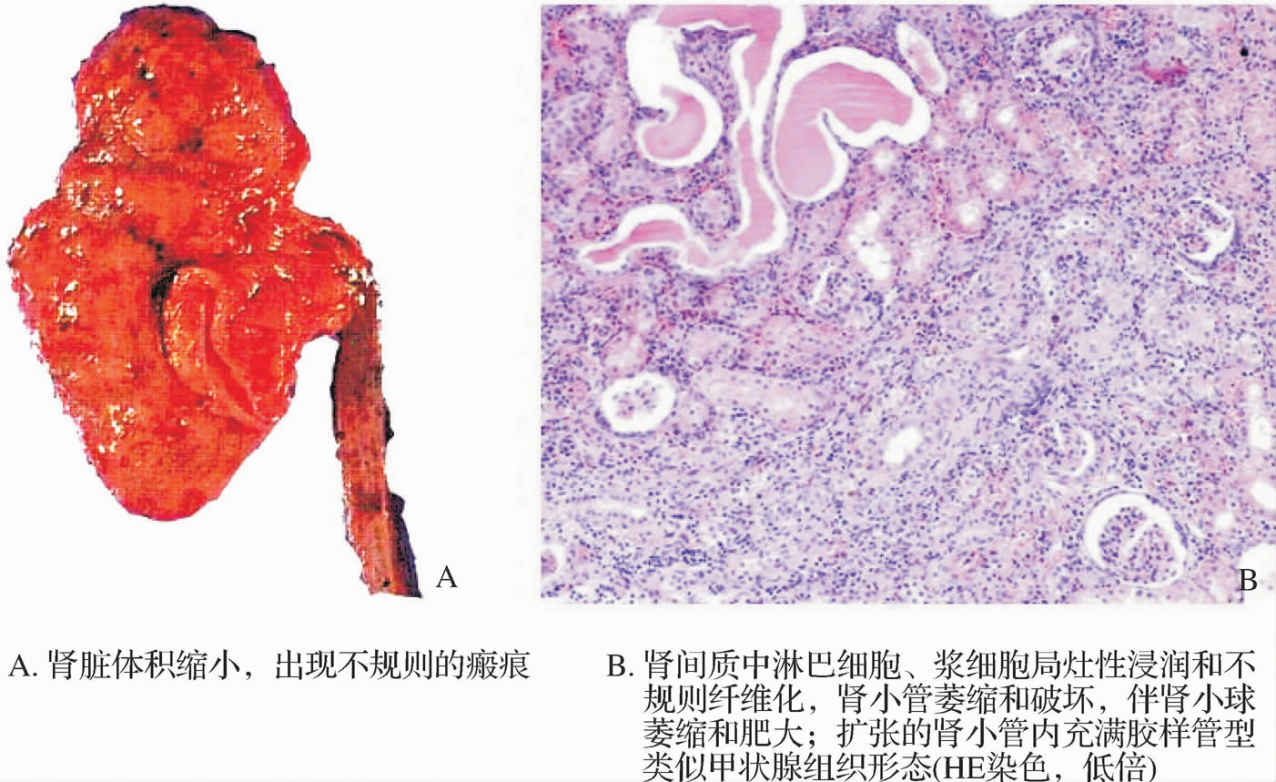
\includegraphics{./images/Image00176.jpg}
 \captionsetup{justification=centering}
 \caption{慢性肾盂肾炎}
 \label{fig10-27}
  \end{figure} 

尽管慢性肾盂肾炎的多数病例可追溯到急性病史,有持续或反复的细菌感染,但有相当数量的慢性病例与先前的急性发病阶段无关。尤其需注意的是不伴有尿路堵塞的慢性肾盂肾炎的病人,通常没有以前或当前受感染的证据。这种病例不能排除先前已有无症状性细菌感染的可能性,还提示可能有除了感染以外的其他因素可引起本病。

\paragraph{临床病理联系}
慢性肾盂肾炎常反复发作,伴有腰背部疼痛、发热,频发的脓尿和菌尿。肾小管功能特别是浓缩能力的丧失会导致多尿和夜尿。钠、钾和重碳酸盐丧失可引起低钠、低钾及代谢性酸中毒。肾组织纤维化和小血管硬化导致局部缺血,肾素分泌增加,引起高血压。晚期肾组织破坏严重,出现氮质血症和尿毒症。X线检查可显示不对称的固缩肾,伴有典型的粗糙瘢痕、肾盂肾盏变平和变形。菌尿是本病的特征,但在终末阶段常消失。肾盂造影术和X线检查均有助于本病的诊断。

\paragraph{预后}
若能及时去除诱发因素,病变可获控制,肾功能可获代偿而不引起严重后果。若频繁发作并广泛累及双肾,最终必将引起慢性肾衰竭(占11%~20%)和高血压,危及生命。一些伴有肾盂肾炎瘢痕的病人可在数年后发展为局灶性节段性肾小球硬化,预后多不佳。

\subsection{药物和中毒引起的肾小管-间质性肾炎}

抗生素和镇痛药的广泛应用已使药物成为引起肾脏损伤的主要原因之一。药物和中毒可诱发间质的免疫反应,引起双侧非化脓性肾间质病变,称为急性过敏性间质性肾炎,也可造成肾小管的慢性损伤,最终导致慢性肾功能不全。

\subsubsection{急性过敏性间质性肾炎}

急性过敏性间质性肾炎,又名急性药物性间质性肾炎,过敏性急性小管间质性肾炎、变应性小管间质性肾炎、急性过敏性小管间质性肾炎等,是常见的免疫介导的肾脏损害。

\paragraph{病因和发病机制}
目前发现引起急性过敏性间质性肾炎的药物种类很多,可由抗生素、利尿药、非甾体抗炎药(NSAIDs)及其他药物引起。抗生素引起的占2/3,常见的如氨基糖苷类、青霉素类、头孢菌素类、两性霉素、四环素族、磺胺类、阿霉素、抗结核药等。利尿药如噻嗪类、呋塞米、三氨苯蝶啶、氯噻酮。NSAIDs如吲哚美辛、布洛芬、阿司匹林等。其他药物如抗癫痫药物、麻醉剂、中枢兴奋剂、免疫抑制剂等。

急性药物性间质性肾炎主要由免疫机制引起。药物作为半抗原与肾小管上皮细胞胞质或细胞外成分结合,产生抗原性,引起IgE的形成和(或)细胞介导的免疫反应,导致肾小管上皮细胞和基膜的免疫损伤和炎症反应。

\paragraph{病理变化}
肾间质出现严重的水肿、淋巴细胞和巨噬细胞浸润,并有大量嗜酸性粒细胞(图\ref{fig10-28})和中性粒细胞,可有少量浆细胞和嗜碱性粒细胞。新型青霉素I和噻嗪类利尿药等药物可引起具有巨细胞的间质肉芽肿性改变。肾小管出现不同程度的变性和坏死。肾小球通常不受累,但非甾体抗炎药引起的间质性肾炎可伴有微小病变性肾小球病和肾病综合征。

\begin{figure}[!htbp]
 \centering
 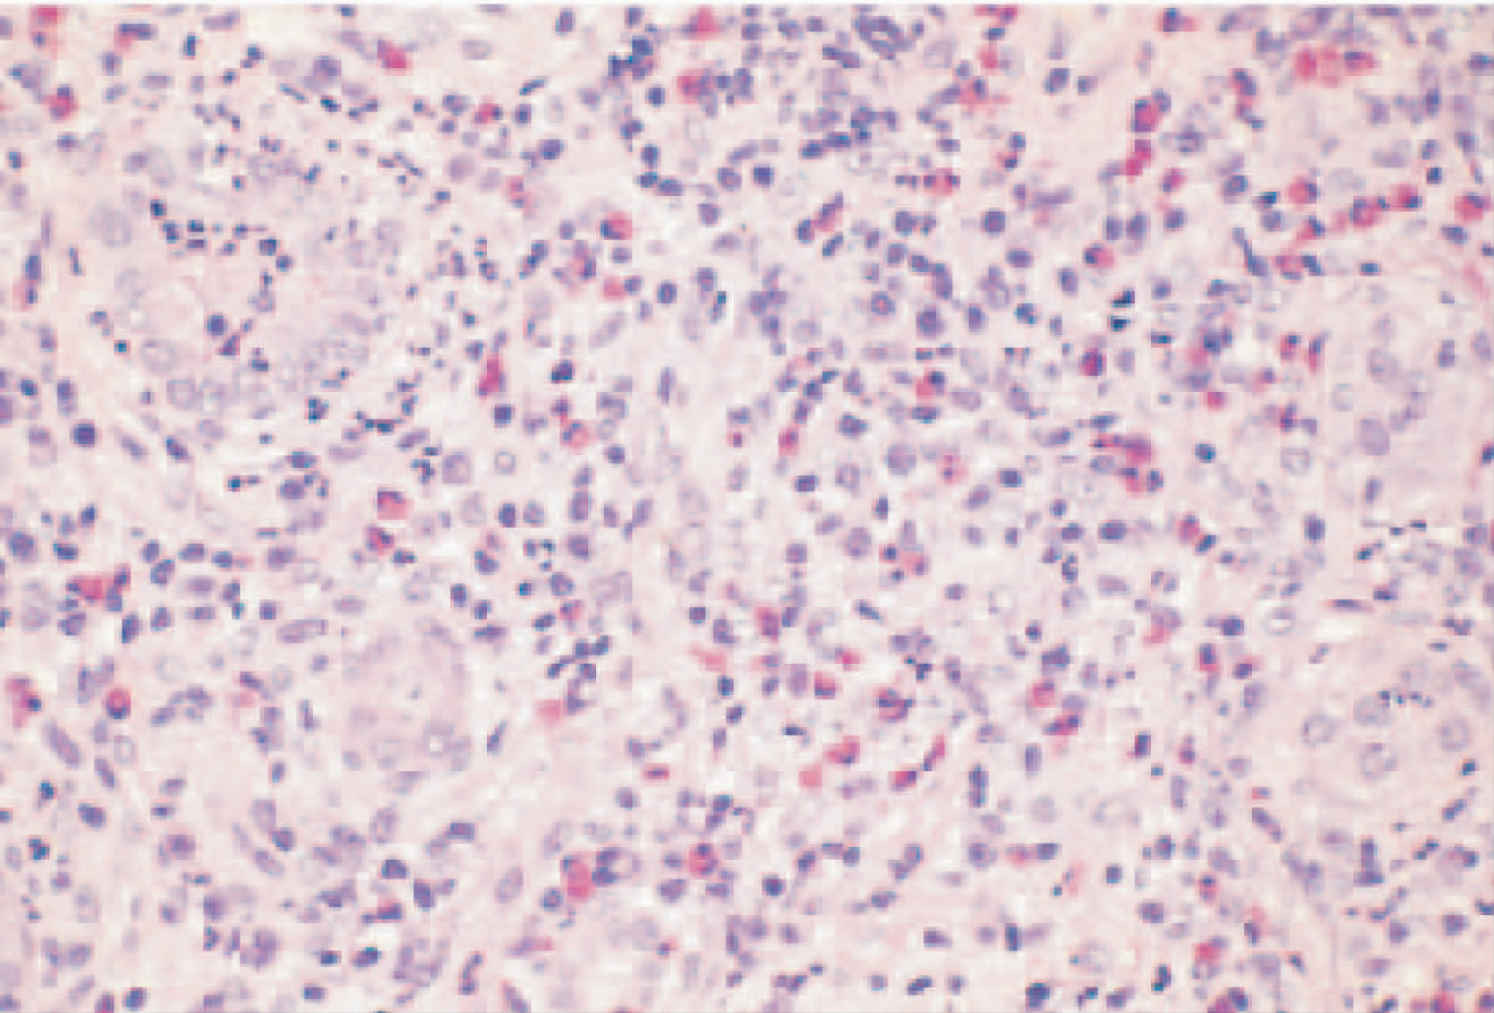
\includegraphics{./images/Image00177.jpg}
 \captionsetup{justification=centering}
 \caption{药物诱导性间质性肾炎(HE染色,高倍)\\ {\small 病变显示小管间质水肿、中性粒细胞、嗜酸性粒细胞浸润}}
\label{fig10-28}
  \end{figure}

\paragraph{临床病理联系}
病变可发生于任何年龄,常在用药后2~40天(平均15天)出现发烧、皮疹(占25%)、关节痛、一过性嗜酸性粒细胞增高等症状(占60%~80%)。肾脏病变引起血尿(占95%)、轻中度蛋白尿和白细胞尿,且86%的尿白细胞中嗜酸性粒细胞占30%以上。约50%病人血清肌酐水平增高,也可出现少尿等急性肾衰竭的症状。但非甾体抗炎药引起的本病主要发生在老年人(64.6岁±2.1岁),常发生在数月之后,只有5%的患者有嗜酸性粒细胞尿,24小时尿蛋白定量小于1.5
g。短时间的嗜酸性粒细胞增多,对本病诊断有较大帮助。

\paragraph{预后}
及时停用相关药物后病情可缓解,但常需要几个月的时间肾功能才能完全恢复正常。少数老年病人的肾脏功能难以恢复。常见并发症主要为代谢性酸中毒、心衰及急性肾衰竭。

\subsubsection{镇痛药性肾炎}

镇痛药性肾炎,又称镇痛药性肾病,是由于病人长期或大量混合服用镇痛药,其累积量超过1~2
kg时引起的慢性肾脏疾病,病变特点是慢性肾小管-间质性炎症和(或)肾乳头坏死。也称镇痛剂所致慢性小管间质性肾炎、无痛性肾病。

\paragraph{病因和发病机制}
常见的引起镇痛药肾病的药物有对乙酰氨基酚、阿司匹林、非那西汀等混合镇痛药等。

发病原因为病人长期或大量服用至少两种镇痛药,累积量超过1~2
kg时,即可患病,累积量超过6
kg者肾脏受累可达50%~80%。发病机制主要是复方镇痛药中部分成分如对乙酰氨基酚在肾髓质中堆积,并在由细胞色素P-450系统参与的代谢过程中生成过多的活性氧成分,同时抑制前列腺素合成,引起肾血流量减少,肾小球滤过率下降导致肾缺血性肾乳头坏死,还可引起肾组织的直接毒性作用和局部过敏反应及肾小血管硬化,肾乳头损伤是药物的毒性作用和缺血共同作用的结果。此外,细胞凋亡可能也参与慢性间质性肾炎的发生。

\paragraph{病理变化}
肉眼上双肾体积正常或轻度缩小。肾皮质厚薄不一。坏死乳头表面皮质下陷。肾乳头发生不同程度的坏死、钙化和脱落。镜下肾乳头早期出现灶状坏死。严重时整个肾乳头坏死,局部结构破坏,仅见残存的肾小管轮廓,并有灶状钙化。有的肾乳头从肾脏剥脱。皮质肾小管萎缩,间质纤维化并有淋巴细胞和巨噬细胞浸润。

\paragraph{临床病理联系}
临床常表现为慢性肾衰竭、高血压和贫血。贫血可能与镇痛药代谢产物对红细胞的损伤有关。实验室检查显示尿浓缩功能减退。肾乳头坏死可引起肉眼血尿和肾绞痛。磁共振和CT检查可显示肾乳头坏死和钙化。

\paragraph{预后}
停用相关镇痛药可使病情稳定,并可能使肾功能有所恢复。少数镇痛药性肾炎的病人有肾盂的移行细胞癌的危险。主要并发症有:

(1)肾结石和慢性肾功能不全:本病约60%病人伴发尿路感染。晚期可能有慢性肾功能减退,表现为少尿型肾衰。

(2)消化道主要并发症为胃及十二指肠球部溃疡、消化道出血、胃穿孔及幽门梗阻等。

(3)心血管系统主要并发症是心脏扩大,心力衰竭及恶性高血压等。

另外,可使皮肤呈青铜色以及精神紧张、抑郁、心理障碍等。

\subsubsection{马兜铃酸肾病}

自1964年首次由吴松寒报道了两例病人因服用大剂量关木通导致急性肾衰竭以来,我国陆续有学者报道了该病。1993年比利时学者Vanherweghem等首先报道了服用含马兜铃属中药广防己的“苗条丸”导致的肾衰竭,并将此称为“中草药肾病”。以后其他国家也有类似的报道。1999年后,我国学者又陆续报道了马兜铃类植物所致的肾病病例,并提出马兜铃酸可能是引起所谓的“中草药肾病”的主要毒性物质,将其命名为马兜铃酸肾病。由于马兜铃酸肾病的临床表现较特殊,发展较快,危害较大,目前其发病机制不清,治疗无成熟方案,因此很有必要提高对此病的认识。

\paragraph{病因和发病机制}
马兜铃属植物广泛分布于热带和亚热带,我国有40余种。常用于中药的包括马兜铃、青木香、天仙藤、广防己、汉中防己、关木通和寻骨风等。这些植物均含有马兜铃酸。目前已知马兜铃酸引起的肾病有三种形式,但其发病机制不清,分别为①急性马兜铃酸肾病(短期大量服用关木通煎剂引起);②肾小管功能障碍型马兜铃酸肾病(间断小量服用后数月发病);③慢性马兜铃酸肾病(在持续或间断服用后),后二者主要是由服用含关木通、广防己或青木香的中成药所致。

\paragraph{病理变化}
(1)急性马兜铃酸肾病:病理学特征是急性肾小管坏死。部分肾小管仅残留裸露基膜,肾间质水肿,偶有少量淋巴细胞、单核细胞浸润,肾小球无明显病变,小动脉内皮细胞肿胀。部分病人有肾小球系膜轻度增生病变。

(2)肾小管功能障碍型:病理改变较轻,主要为肾小管变性及萎缩,部分崩解脱落。管腔扩张,肾间质无明显病变或轻度水肿。肾小球基本正常。

(3)慢性马兜铃酸肾病:肉眼肾小球缩小,双肾可不对称,镜下显示有慢性肾间质纤维化,特点为多灶或大片状纤维化,有少量淋巴、单核细胞呈散在或灶性浸润,白细胞浸润不明显,故称为寡细胞性肾间质纤维化。

\paragraph{临床病理联系}
急性马兜铃酸肾病表现为急性肾衰竭,死亡率高。临床表现为少尿或非少尿性急性肾衰,恶心、呕吐、贫血、血小板减少、肝功能损害,视力、听力障碍、震颤等。

肾小管功能障碍型马兜铃酸肾病主要表现为肾小管酸中毒和(或)Fanconi综合征,伴轻度蛋白尿及肾浓缩功能障碍,而血清肌酐及尿素氮基本正常。

慢性马兜铃酸肾病多数病例起病隐匿,服药后数年出现氮质血症或慢性肾衰竭,少数病例进展迅速,主要表现为肾性糖尿、轻度蛋白尿,低比重及低渗透压尿,肾功能进行性损害(0.5~10年),直到肾衰竭尿毒症。常伴贫血和高血压。

\paragraph{预后}
对本病尚无成熟治疗方案。应先停用马兜铃类药物。皮质激素对早、中期患者可能有缓解病情的作用,其余为对症治疗。马兜铃属药物累积量大时,病人肾盂、输尿管和膀胱癌的发病率增高,应予注意。

\section{肾和膀胱的常见肿瘤}

\subsection{肾细胞癌}

肾细胞癌又称肾癌,是最常见的成人肾脏恶性肿瘤,占肾恶性肿瘤的80%~90%,占成人恶性肿瘤的1%~3%,多发生于40岁以后,男∶女为2∶1。因该肿瘤起源于肾小管上皮,故又称肾腺癌。

\subsubsection{病因和发病机制}

流行病学研究显示在烟草、烟斗和雪茄的吸烟者中肾细胞癌是非吸烟者的两倍,因此吸烟被认为是肾细胞癌最重要的危险因子,但有家族倾向。资料显示其散发性病例占绝大多数,发病年龄大,多发生于一侧肾脏。而遗传性、家族性肾细胞癌为常染色体显性遗传,仅占4%,发病年龄小,肿瘤多为双侧多灶性。其他危险因素还有肥胖(特别是女性)、高血压、接触石棉、石油产品和重金属等。

在发病机制中,几乎所有的遗传性肾癌和绝大多数的散发性肾透明细胞癌源于VHL(Von
Hippel-Lindau)基因的异常。VHL基因是一种抑癌基因,位于染色体3的短臂上(3p25~26),编码一种信号传导或细胞黏附的蛋白质,参与调控细胞生长。该基因的缺失、易位、突变或高甲基化均与肾透明细胞癌的发生有关。肾透明细胞癌散发和遗传性病例均有染色体3p的缺失。缺失区域含有VHL基因。80%的肾透明细胞癌病人的未缺失的VHL等位基因发生突变或高甲基化性失活。在非乳头状肾癌的遗传性、家族性病例中常发现VHL基因的3∶8或3∶11基因易位。肾细胞癌有近2/3病例伴有VHL综合征,表现为中枢神经系统和视网膜出现血管母细胞瘤,可发生双侧多灶性的肾细胞癌。乳头状肾癌与VHL基因改变无关。散发性乳头状肾细胞癌的细胞遗传学改变主要是7,16和17号染色体三体性及男性患者的y染色体丢失,检测到7号染色体位点MET基因酪氨酸激酶结构域的突变。遗传性、家族性乳头状肾癌的改变主要是7号染色体三体性;散发性乳头状肾癌存在1号染色体的乳头状肾细胞癌基因与位于X染色体的转录因子E3基因融合。嫌色细胞癌常显示多个染色体缺失和亚二倍体。

\subsubsection{病理变化}

\paragraph{肉眼观}
肿瘤常为单个圆形,直径为3~15
cm,多见于肾上、下两极,但以上极更多见。乳头状癌可为多灶和双侧性。切面呈淡黄色或灰白色,可见结缔组织小梁,常伴变性、坏死、软化、出血和囊性变,因此表现为红、黄、灰、白等多种颜色相交错的多彩的特征(图\ref{fig10-29})。肿瘤边缘通常境界清晰,可有假包膜形成,局限于肾包膜内。在肿瘤周围常出现小的卫星灶样癌结节,这证明肿瘤具有侵袭性,其侵袭性的一个最显著特征是肿瘤可蔓延到肾盂、肾盏和输尿管,并常侵犯肾静脉形成瘤栓,肾静脉瘤栓可进一步延伸至下腔静脉,甚至右心。偶尔直接浸润到肾周脂肪中或肾上腺。

\begin{figure}[!htbp]
 \centering
 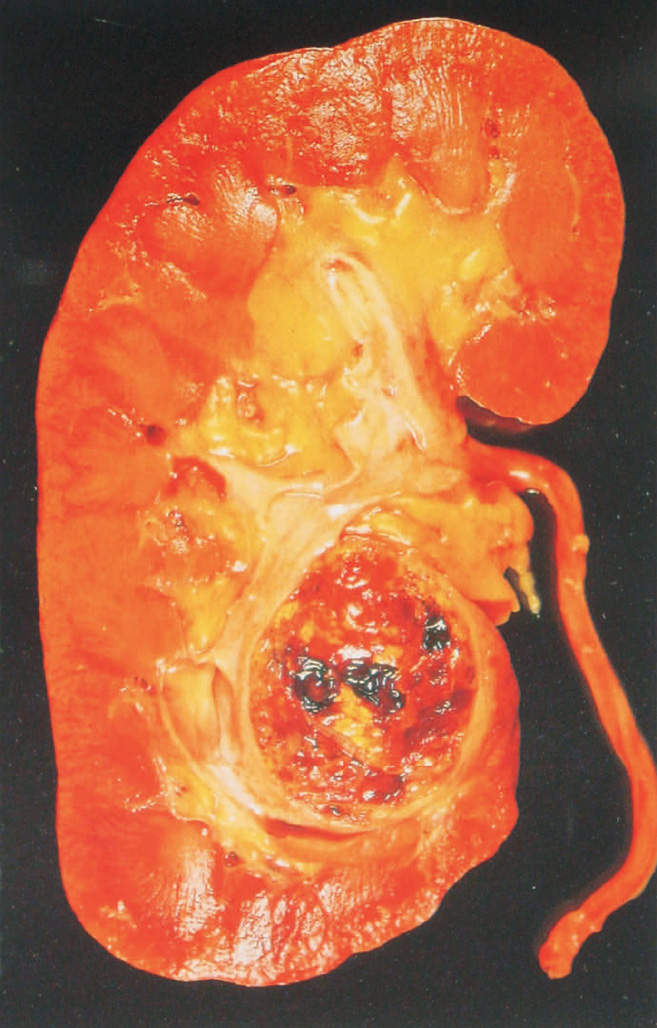
\includegraphics{./images/Image00178.jpg}
 \captionsetup{justification=centering}
 \caption{肾细胞癌\\ {\small 境界清楚的肾细胞癌压迫肾盂。肿瘤呈淡黄色伴出血}}
\label{fig10-29}
  \end{figure}

\paragraph{镜下}
光镜下,肿瘤生长模式多种多样,有乳头状、实性小梁状(条索样)或管状(似小管样)。可根据细胞的形态将肾细胞癌分为透明细胞型、颗粒细胞型、肉瘤样细胞癌。肉瘤样细胞癌较少见,主要由未分化的肿瘤细胞构成。近来,基于对家族性和散发性肾细胞癌的细胞遗传学、遗传学和组织病理学的综合研究,修订了新分类主要类型。

(1)肾透明细胞癌:占肾细胞癌的70%~80%,是最常见的肿瘤细胞类型。肿瘤细胞体积较大,呈圆形或多角形,胞质丰富,透明或颗粒状,核小常被推到基底侧,胞质PAS特殊染色阳性(图\ref{fig10-30}A)。

(2)乳头状肾细胞癌:多为多中心起源,占肾细胞癌的10%~15%。肿瘤细胞呈立方状或矮柱状、乳头状排列。乳头中轴间质内常见砂粒体和泡沫细胞,并可发生水肿(图\ref{fig10-30}B)。

(3)嫌色性肾细胞癌:在肾细胞癌中约占5%。肿瘤细胞大小不一,细胞膜较明显,胞质淡染或略嗜酸性,核周常有空晕(图\ref{fig10-30}C)。病人预后较好。细胞遗传学检查常显示多个染色体确实或亚二倍体细胞,

(4)其他类型:包括集合管癌(图\ref{fig10-30}D)和未分类性肾癌。前者较少见,在肾癌中的比例不到1%。后者为不能归入其他类型的肾癌,占肾细胞癌的3%~5%。

\begin{figure}[!htbp]
 \centering
 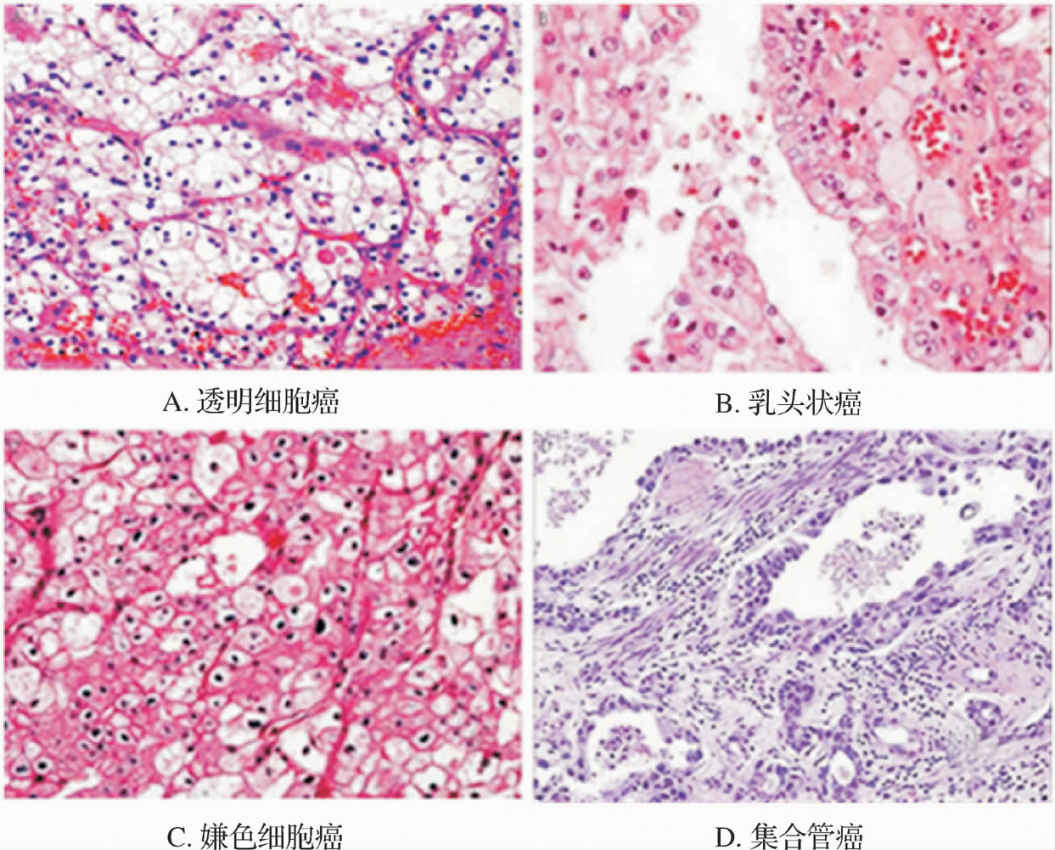
\includegraphics{./images/Image00179.jpg}
 \captionsetup{justification=centering}
 \caption{肾细胞癌的细胞学类型}
 \label{fig10-30}
  \end{figure} 

\subsubsection{临床病理联系}

肾细胞癌早期症状不明显,主要为血尿,占肾细胞癌患者的50%以上。肉眼血尿呈间歇性或瞬间性,镜下血尿较稳定出现。有些患者由于肿瘤体积增大引起腰部疼痛和出现可触及的肿块。腰痛、肾区肿块和血尿是本病具有诊断意义的三个典型症状,简称“三联征”,但三者同时出现的比例很小。常见的肾外表现有发热和红细胞增多症,后者占肾细胞癌患者的5%~10%,这是由于肾肿瘤产生红细胞生成素增加所致。肾肿瘤也可能产生一些激素样物质引起高钙血症、高血压、Cushing's综合征或女性化、男性化的表现,但这些表现并不常见。

肾细胞癌具有广泛转移的特征,常在局部症状和体征出现前就已发生了转移,因此许多患者在肿瘤转移产生症状时才被发现。肾细胞癌最常见的转移部位是肺(超过50%)和骨(33%),接下来依次为局部淋巴结、肝、肾上腺和脑。在10%~15%的病例中原发肿瘤可越过中线转移至对侧肾脏。通过放射检查可发现25%的转移病灶。肾超声检查、肾体层摄影、CT扫描和静脉内肾盂造影术有助于鉴别诊断单纯囊肿和肿瘤。尿液脱落细胞学检查可有助于识别肿瘤细胞。

\subsubsection{预后}

肾癌病人预后较差,5年生存率约为45%,若无远处转移可达70%以上。随着肿瘤侵入肾静脉和肾周脂肪组织,5年生存率降至15%~20%。

\begin{framed}
{案例10-2}

{【病例摘要】}

晋×,男性,58岁。无痛性血尿一周。体检:血压150/100
mmHg,呼吸20次/分,心率78次/分。实验室检查:血红细胞6×10{12}
/L,血白细胞6.9$\times 10^{9}$
/L,尿沉渣红细胞3+,肾功检查无异常。肾区CT检查显示:肾上极包块。自诉有长期吸烟史,但无高血压、糖尿病、肾炎等病史。

{【问题】}

(1)试问本病最可能的诊断是什么?

(2)单纯无痛性血尿应考虑哪些病?
\end{framed}

\subsection{肾母细胞瘤}

肾母细胞瘤又称肾胚胎瘤,是起源于后肾胚基组织的恶性肿瘤,因最早由Max
Wilms医师于1899年首先描述,故又称Wilms瘤,在10岁以内儿童癌症好发器官中居第三位,是儿童期肾脏最主要的恶性肿瘤之一,也是应用现代综合治疗最早和效果最好的恶性实体瘤。肿瘤多发生于儿童,其中有90%发生于7岁前,平均年龄是15个月,罕见于成人及新生儿。男女性别及肾左右侧的发病率无明显差别。

\subsubsection{病因和发病机制}

从胚胎学上来说,肾母细胞瘤是由于持续存在的后肾胚基未能分化为肾小球及肾小管并呈不正常的增殖发展形成。肿瘤多数呈散发性,也有家族性病例的报道(占1%~2.4%),以常染色体显性方式遗传,伴不完全外显性。有人认为家族性遗传形式显现的肿瘤发生更早,更易为双侧性及多中心形式。发病机制中肾母细胞瘤与WT1基因(Wilms'tumor
associated
gene-1)的缺失和突变有关。WT1基因位于染色体11的短臂上(11p13),编码转录因子,表达于胎儿期肾脏和性腺。根据细胞所处的环境,该基因分别起转录激活和抑制的作用。WT1功能缺失的转基因小鼠肾脏和性腺发育均有障碍。约有15%的散发性Wilms瘤病人中可检测到WT1的突变。Wilms瘤也可由其他遗传学异常引起。Beckwith-Wiedemann综合征病人发生11p15的缺失,许多散发性肾母细胞瘤也发生11p15的杂合性缺失,而11p13位点未被累及。现推测11p15是具有另一个与肾母细胞瘤有关的WT2基因,但有待进一步研究证实。

此外,部分病人伴有不同的先天畸形。已发现的畸形有虹膜缺如(1.1%)、泌尿生殖系畸形(4.4%),如尿道下裂、假两性畸形、隐睾症、单侧肢体肥大(2.9%)等。这些畸形常以三种先天畸形综合征形式出现:分别为:①WAGR综合征:表现为Wi1ms瘤、虹膜缺如、生殖泌尿道畸形和智力迟钝。病人有染色体11p13的缺失,因而缺乏抑癌基因WT1;②Denys-Drash综合征:特点为性腺发育不全(如男性假两性畸形)和幼年发生的肾脏病变(如弥漫性肾小球系膜硬化)并导致肾衰竭。遗传学异常主要是WT1基因的突变;③Beckwith-Wiedemann综合征:特征为器官肥大、巨舌、偏身肥大、脐突出和肾上腺皮质细胞肥大。常可检测到染色体11p15.5的缺失。故对这些小儿应随访监测,如每3个月做一次超声检查,直至5~6岁。

\subsubsection{病理变化}

\paragraph{肉眼观}
肾母细胞瘤多表现为单个实性肿物,体积较大(图\ref{fig10-31}),可仅限于肾区,大者可上起膈下,下达盆腔,跨越中线并使主动脉和下腔静脉(inferior
caval
vein)移位。边界清楚,可有假包膜。少数病例为双侧性和多灶性。肿瘤质软,切面鱼肉状,灰白或灰红色,伴灶状出血或坏死时则呈橘黄色或棕色,间有囊腔形成。约5%病例合并钙化,多位于既往肿瘤坏死区,呈线状位于瘤体周缘,与神经母细胞瘤之分散钙化点不同。罕见肾外肾母细胞瘤,可位于腹膜后或腹股沟区,其他部位包括后纵隔、盆腔和骶尾区。

\begin{figure}[!htbp]
 \centering
 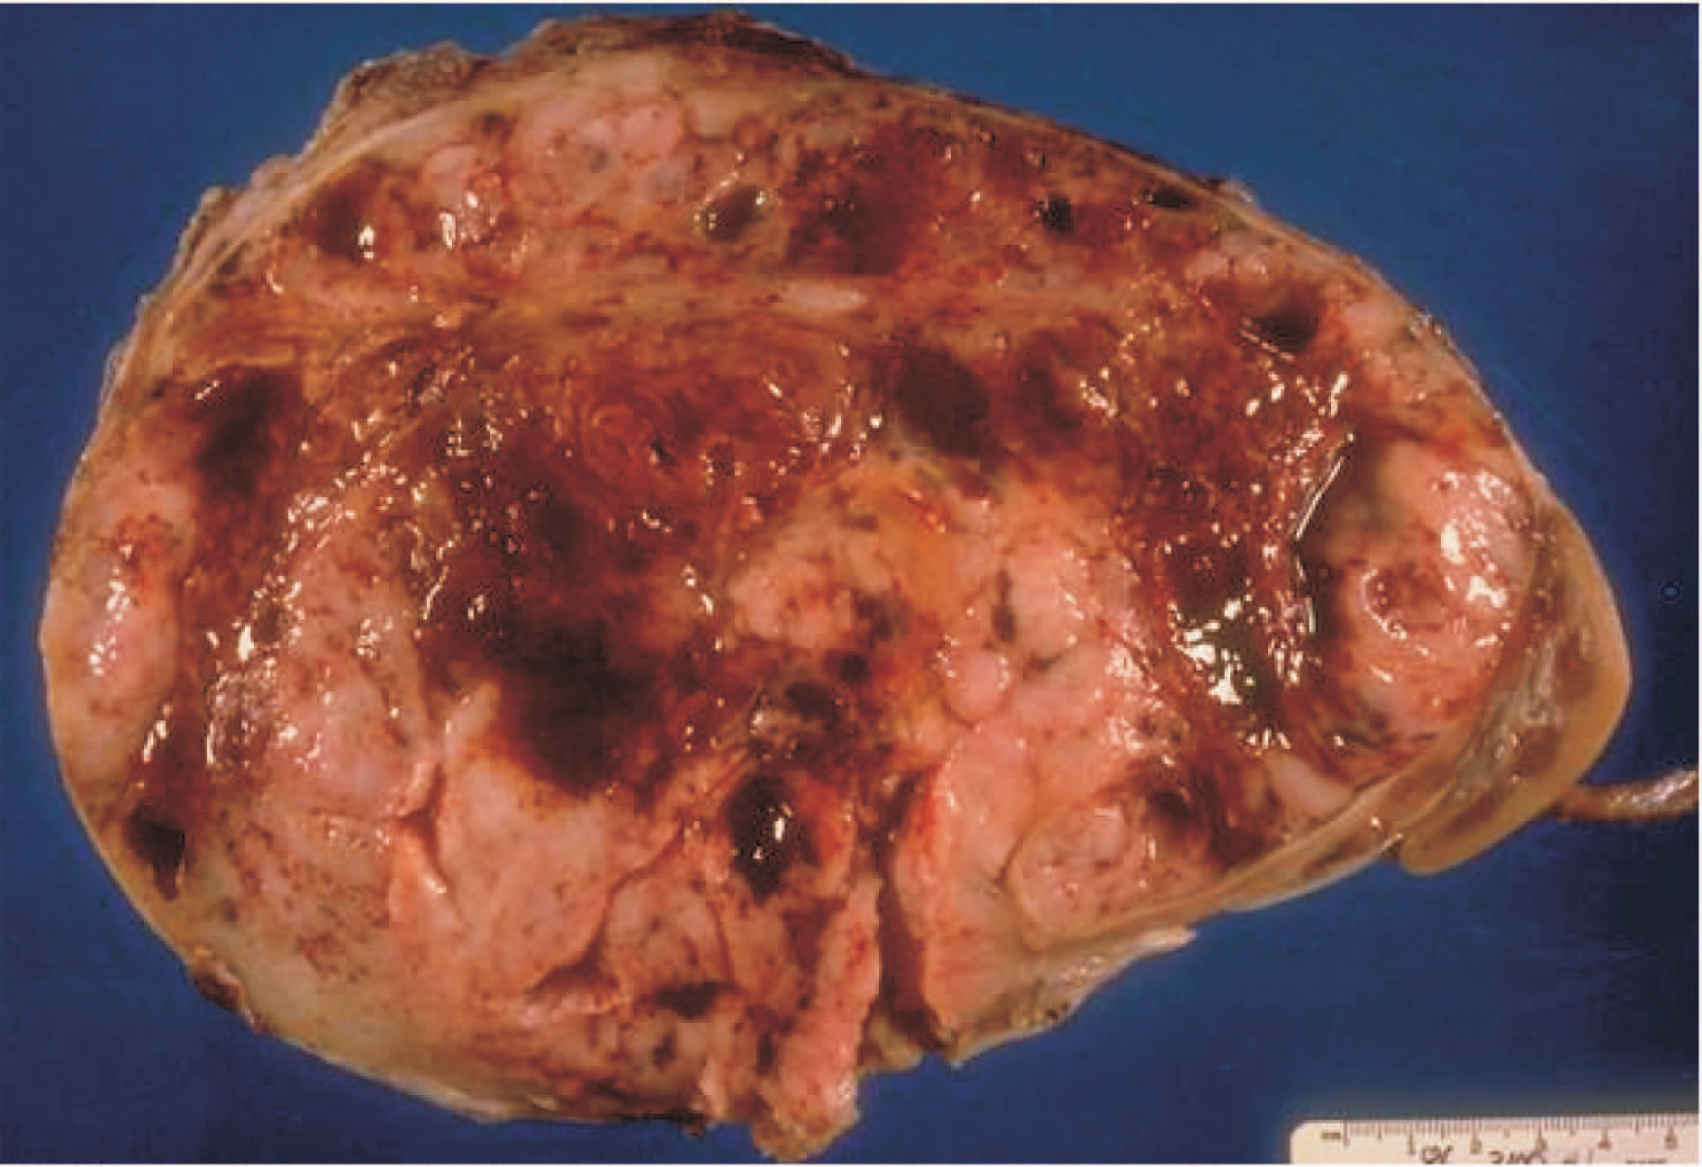
\includegraphics{./images/Image00180.jpg}
 \captionsetup{justification=centering}
 \caption{Wilms瘤\\ {\small 肾脏几乎完全被黄褐色肉质肿瘤取代,肿瘤伴区域性出血和坏死,有假包膜;右边有一小块残留的肾组织,上见输尿管}}
\label{fig10-31}
  \end{figure}

\paragraph{镜下}
肿瘤实质含三种细胞成分,分别为间叶细胞、上皮样细胞和幼稚的胚基组织细胞(图\ref{fig10-32})。上皮样细胞体积小,圆形、多边形或立方形,可形成小管或小球样结构,并可出现鳞状上皮分化;间叶细胞多为纤维性或黏液性,细胞较小,梭形或星状,可出现横纹肌、软骨、骨或脂肪等分化;胚基幼稚细胞为小圆形或卵圆形原始细胞,胞质少。肿瘤间质可含任何结缔组织包括肌肉、软骨等成分,偶见骨组织。

\begin{figure}[!htbp]
 \centering
 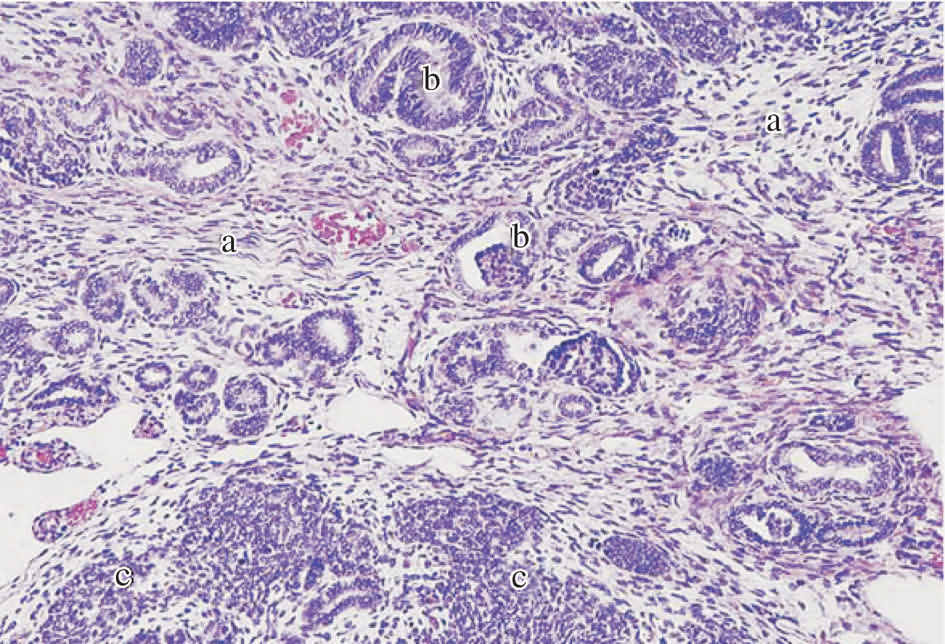
\includegraphics{./images/Image00181.jpg}
 \captionsetup{justification=centering}
 \caption{肾母细胞瘤\\ {\small 肿瘤实质含三种细胞成分,分别为间叶组织的细胞(a)、上皮样细胞(b)和幼稚的胚基组织细胞(c)}}
\label{fig10-32}
  \end{figure}

病理类型:肾母细胞瘤分预后好的组织类型和预后差的组织类型两类,预后好的为经典型肾母细胞瘤,易于辨认。预后差的为未分化型,局灶或弥散性,瘤细胞较经典型者大三倍,核深染,较多病理性核分裂象。

\subsubsection{临床病理联系}

腹部肿块是最常见的症状,约75%患者均以腹部肿块或腹胀就诊。肿块位于上腹季肋部一侧,表面平滑,中等硬度,无压痛,早期可稍具活动性,迅速增大后,少数病例可超越中线。此时虽无远距离转移,但小儿受巨大肿瘤压迫,可有气促、食欲不振、消瘦、烦躁不安现象。肉眼血尿少见,但镜下血尿可高达25%。25%~63%的患者有高血压,肿瘤切除后,血压可恢复正常。此外,偶见腹痛及低热,但多不严重。食欲不振、体重下降、恶心及呕吐是疾病晚期的信号。肿瘤也可产生红细胞生长素导致红细胞增多症。极少数肾母细胞瘤自发破溃,临床上与急腹症表现相似。

\subsubsection{预后}

采用手术配合化疗及放疗的综合疗法能取得良好的效果。完整执行治疗方案的病例,2年无复发可认为治愈;治疗方案执行不完整的要等待5年再作定论。肿瘤局限在肾内者,2年无瘤存活率为88%,2年存活率为93%。局部晚期病变及远处转移者,2年无瘤存活率为77%。从组织类型分析,预后好的2年存活率为90%,预后差的仅54%。

\subsection{膀胱尿路上皮肿瘤}

膀胱肿瘤约有95%来源于上皮组织,其中最常见的来源于尿路上皮即移行上皮,称为尿路上皮肿瘤或移行上皮肿瘤,其他也可发生鳞状细胞癌、腺癌和间叶起源的肿瘤,但均较少见。

膀胱尿路(移行)上皮癌是世界上第七位最常见的恶性肿瘤,估计每年全世界新增病例为男性26万,女性7.6万,膀胱癌占全世界所有癌肿的3.2%,男性多于女性(男∶女约3∶1),在两性中膀胱尿路上皮癌的最高发病率在西欧、北美和澳洲。总的来说,发达国家的发病率高于发展中国家,城市居民发病率高于农村人口,发病多数在50岁以后。

膀胱尿路上皮癌约占整个膀胱癌的男性84%、女性79%,所以以下介绍的主要为膀胱尿路上皮癌。

\subsubsection{病因和发病机制}

\paragraph{与膀胱尿路上皮癌发生相关的危险因素}
(1)吸烟:吸烟是膀胱尿路上皮癌最确定的危险因素。据估计,由于吸烟所致的膀胱尿路上皮癌的危险性,在男性为66%,在女性为30%。吸烟者发生膀胱尿路上皮癌的危险性是非吸烟者的2~6倍。随着吸烟时间的延长,发生膀胱尿路上皮癌的危险性增加。

(2)职业暴露因素:膀胱尿路上皮癌与许多职业或职业暴露因素相关。这种相关性最初被Rehu在1895年发现,Rehu认为在从事苯胺印染工业的男性中,膀胱尿路上皮癌的发生率高。随后研究发现对二氨基联苯胺、2-奈胺和1-奈胺都可能是膀胱尿路上皮癌的危险因素。据估计,25%以上的膀胱肿瘤与职业接触致癌物有关。

(3)药物:一些流行病学研究表明长期滥用包括非那西丁(Phenacetin)在内的解热镇痛药很大程度上增加了膀胱尿路上皮癌发生的危险性。其他抗肿瘤药萘氮芥(chlornaphazine)和膀胱尿路上皮癌的发生相关。

(4)慢性感染:由血吸虫导致的慢性膀胱炎是膀胱尿路上皮癌的一个确定病因。一些学者提示膀胱尿路上皮癌与泌尿道感染、泌尿道结石有相关性。基本机制是可能导致膀胱壁的慢性刺激,这种慢性刺激可能增加膀胱尿路上皮癌发生的危险性。

(5)其他因素:一些研究表明饮用含有氯化物和被砷污染的水可能增加膀胱尿路上皮癌发生的危险性。在从未吸烟的仅由饮用咖啡所致的膀胱尿路上皮癌的危险性增加,而长期吸烟且饮用咖啡所致的膀胱尿路上皮癌的危险性没有发现增加。人工甜味佐料也可能增加膀胱尿路上皮癌发生的危险性。

\paragraph{膀胱尿路上皮癌发病机制}
膀胱尿路上皮癌发生的分子模式包括两条途径。第一条途径是通过9号染色体为单体或发生9p和9q的缺失累及p16等抑癌基因的缺失,引起浅表的乳头状肿瘤。一些病例在此基础上发生p53缺失或突变,肿瘤发生浸润。另一条途径是通过17p(含p53基因)的缺失或p53的突变导致原位癌,再发生9号染色体的缺失,发展为浸润癌。许多侵袭性尿路上皮癌中p53基因的改变与癌进展有关。其他改变包括13q缺失累及Rb基因,见于浸润性肿瘤。以及11p和14q的缺失等。

\subsubsection{病理变化}

\paragraph{肉眼观}
膀胱尿路上皮癌好发于膀胱侧壁和膀胱三角区近输尿管开口处。肿瘤可单个或可多灶性,大小不等。肿瘤外观可呈乳头状到扁平状(图\ref{fig10-33}),生物学表现亦可从不伴浸润到浸润,从高分化到高度间变,侵袭性程度各不相等。最具有临床意义的是肿瘤浸润的深度。

\begin{figure}[!htbp]
 \centering
 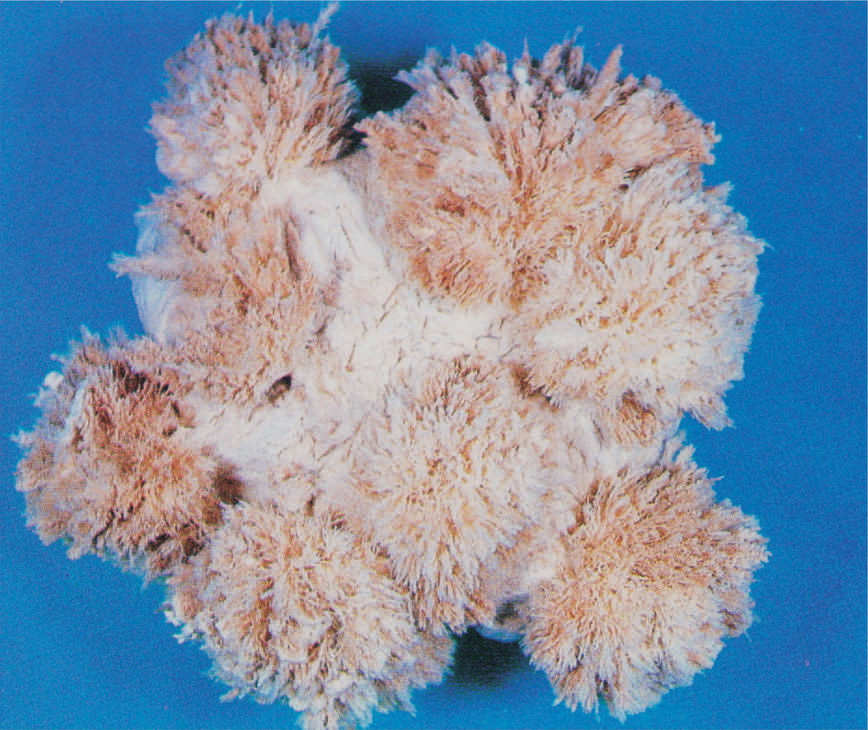
\includegraphics{./images/Image00182.jpg}
 \captionsetup{justification=centering}
 \caption{乳头状尿路上皮(移行细胞)癌\\ {\small 多个息肉样肿块表面被覆无数纤细的乳头}}
\label{fig10-33}
  \end{figure}

\paragraph{镜下}
(1)病理分级:可根据瘤细胞有无间变、细胞大小、核异型、排列方式,将膀胱尿路上皮癌分为Ⅰ级~Ⅲ级。

Ⅰ级:肿瘤细胞有一定异型性,但分化较好,近似于正常的移行细胞,核分裂象少见,细胞层次增多至七层以上,但极性无明显紊乱(图\ref{fig10-34}A)。Ⅰ级癌总是以乳头状方式生长,很少浸润,但可以术后复发。

Ⅱ级:肿瘤细胞仍可识别出起源于移行细胞。细胞层次增多(通常超过十层),且核分裂象较多,极性消失。细胞大小、形态改变明显,核染色深(图\ref{fig10-34}B)。一些肿瘤显示鳞状分化。

Ⅲ级:肿瘤细胞勉强可识别出移行细胞的起源。所有在Ⅱ级中发生的细胞改变更为严重,细胞排列紊乱并伴有细胞表层的松散和碎裂(图\ref{fig10-34}C)。肿瘤可以覆盖膀胱黏膜表面的大部分区域,深部浸润,有蓬松的表面坏死。有时可出现巨细胞。可见近似鳞状细胞和腺细胞癌的方向分化,但仅只有5%的膀胱癌是真正鳞状细胞癌。半数病人有严重的间变,大多数发生于膀胱侧壁、后壁,许多膀胱癌为多中心性。

Ⅰ级属于非浸润性乳头状尿路上皮癌,Ⅱ级和Ⅲ级浸润周围组织,扩散到局部淋巴结,偶尔广泛转移。

\begin{figure}[!htbp]
 \centering
 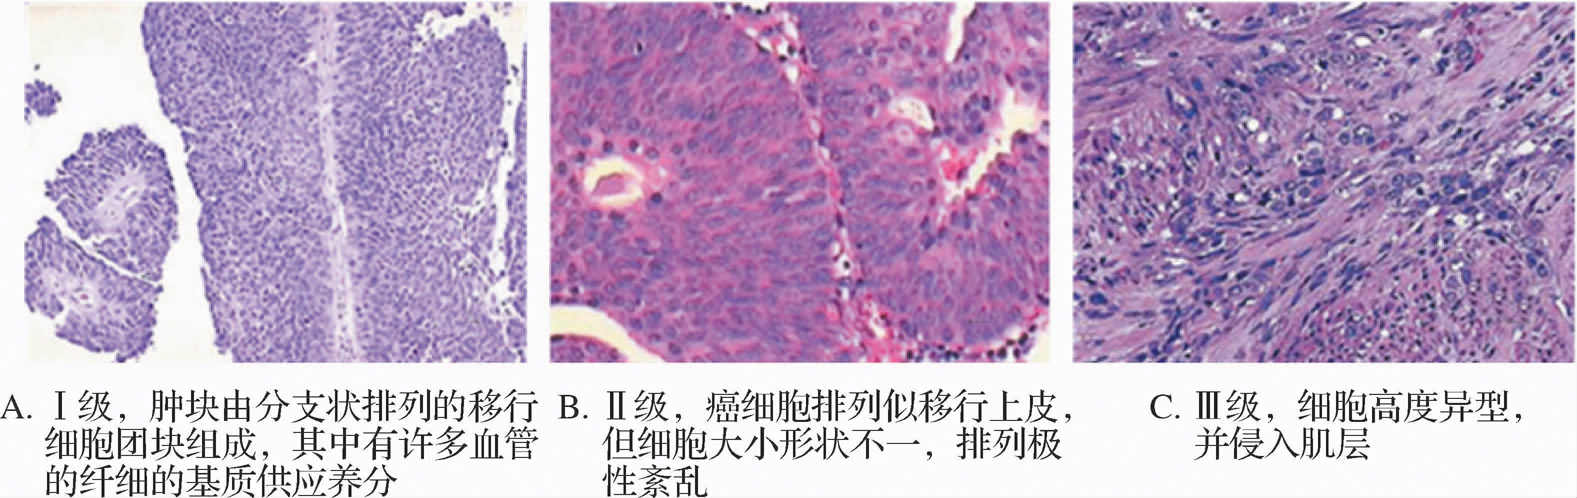
\includegraphics{./images/Image00183.jpg}
 \captionsetup{justification=centering}
 \caption{膀胱乳头状移行细胞癌}
 \label{fig10-34}
  \end{figure} 

(2)浸润性尿路上皮癌的变异型

1)伴有鳞状上皮分化的浸润性尿路上皮癌;

2)伴有腺上皮分化的浸润性尿路上皮癌;

3)巢状癌;

4)微囊癌;

5)微乳头状癌;

6)淋巴上皮瘤样癌;

7)淋巴瘤样和浆细胞样癌;

8)肉瘤样癌(有/没有异源性因素);

9)伴有滋养层细胞分化的移行上皮癌;

10)透明细胞癌;

11)脂质细胞癌;

12)未分化癌:此型非常少见,如小细胞癌、大细胞癌和淋巴上皮瘤样癌,这些肿瘤中的一些类型现被认为是膀胱癌的特殊类型。

(3)世界卫生组织和国际泌尿病理学会对尿路(移形)上皮肿瘤的分类为:①尿路上皮乳头状瘤占膀胱肿瘤的1%或更少,多见于青年。肿瘤呈乳头状,细胞分化好(图\ref{fig10-35}A)。②低恶性潜能的乳头状尿路上皮肿瘤 其组织学特征与乳头状瘤相似,区别是上皮增厚,乳头粗大或细胞核普遍增大(图\ref{fig10-35}B)。③低级别乳头状尿路上皮癌:瘤细胞和组织结构较规则。细胞排列紧密,维持正常极性,但有明显的小灶状核异型性改变,表现为核浓染、少量核分裂象(多见于基底部)和轻度核多形性(图\ref{fig10-35}C)。低级别乳头状尿路上皮癌术后可复发,少数可发生浸润。④高级别乳头状尿路上皮癌 瘤细胞核浓染,部分细胞异型性明显,核分裂象较多,可有病理性核分裂象。细胞排列紊乱,极性消失(图\ref{fig10-35}D)。高级别乳头状尿路上皮癌多为浸润性,并容易发生转移。

\begin{figure}[!htbp]
 \centering
 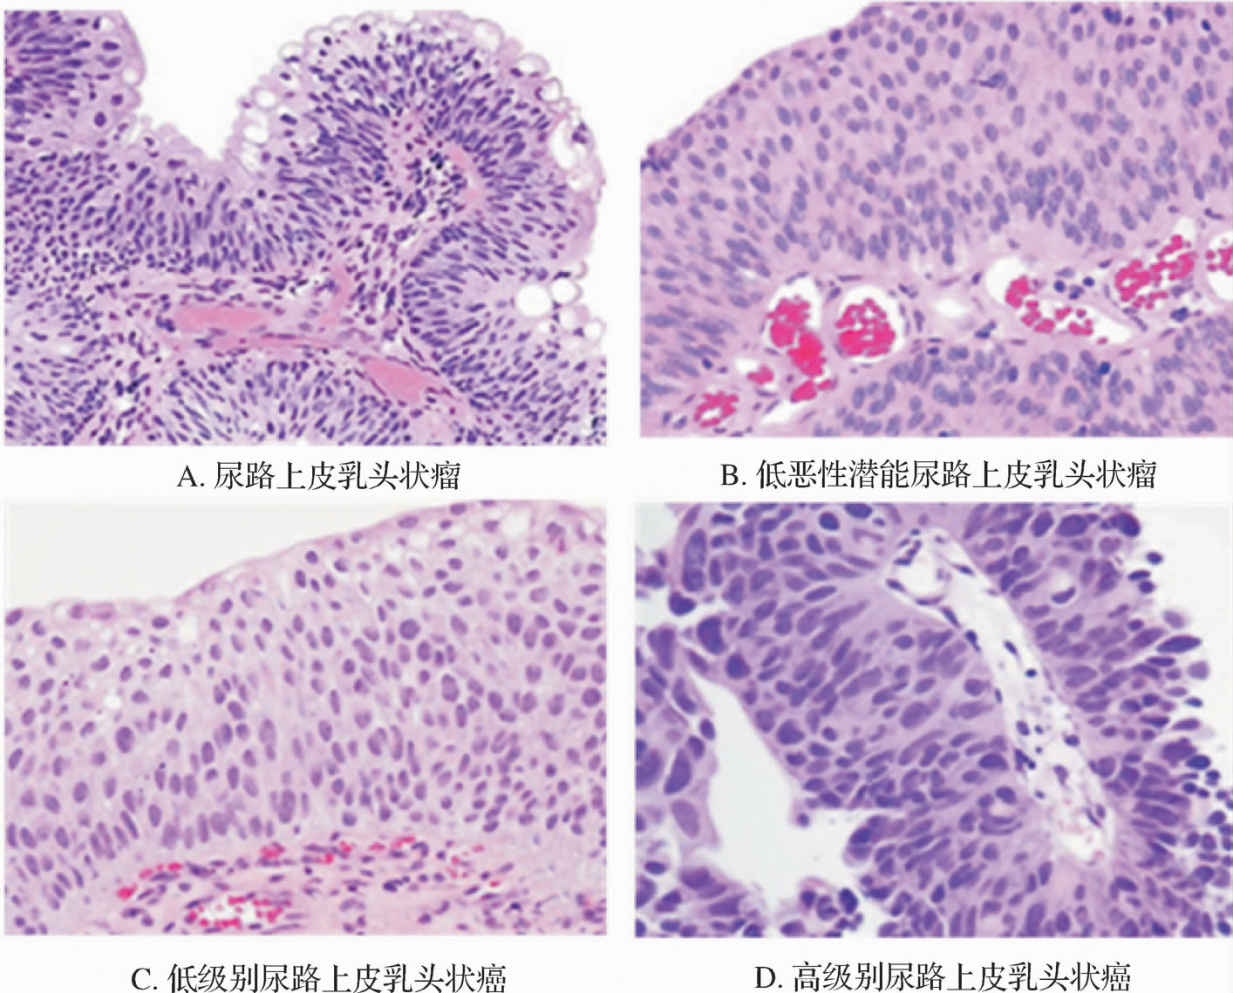
\includegraphics{./images/Image00184.jpg}
 \captionsetup{justification=centering}
 \caption{世界卫生组织(WHO)和国际泌尿病理学会(ISUP)关于尿路上皮肿瘤的分类}
 \label{fig10-35}
  \end{figure} 

据分析,不到10%的低级别膀胱乳头状癌为浸润性,但高级别乳头状癌发生浸润的比例可高达80%。侵袭性强的肿瘤可累及邻近的前列腺、精囊和输尿管等。有的可形成与阴道或直肠相通的瘘管。约40%的浸润性肿瘤可发生局部淋巴结的转移。高度间变的肿瘤晚期可发生血行转移,常累及肝、肺和骨髓。

\subsubsection{临床病理联系}

无痛性血尿是膀胱肿瘤最显著的临床特点,肿瘤乳头的断裂、肿瘤表面坏死和溃疡均可引起血尿。部分病例因肿瘤侵犯膀胱壁,刺激膀胱黏膜或并发感染,出现尿频、尿急和尿痛等膀胱刺激症状。肿瘤阻塞输尿管开口时可引起肾盂积水(hydronephrosis)、肾盂肾炎、甚至肾盂积脓。

\subsubsection{预后}

膀胱尿路上皮起源的肿瘤手术后容易复发,部分复发肿瘤的分化可能变差。

本病总的5年生存率为57%。但尿路上皮肿瘤病人的预后与肿瘤的分级和浸润与否有较密切的关系。乳头状瘤、低恶性潜能乳头状瘤和低级别乳头状癌病人的10年生存率可达90%以上。少数病人(小于10%)进展为高级别肿瘤。而高级别乳头状癌病人的10年生存率仅为40%左右。

\section*{复习与思考}

{一、名词解释}

颗粒性固缩肾 肾炎综合征 肾病综合征 急性增生性肾小球肾炎 快速进行性肾小球肾炎 蚤咬肾 新月体 膜性肾小球病 微小病变性肾小球病 IgA肾病 局灶性节段性肾小球硬化 慢性肾小球肾炎 肾盂肾炎 肾细胞癌

{二、问答题}

1.
慢性硬化性肾小球肾炎肾脏体积缩小及表面颗粒是怎样形成的?它与哪些疾病引起的肾硬变相似?

2. 急性肾小球肾炎与急性肾盂肾炎的发病机制、病理变化和临床表现有何不同?

3. 新月体性肾小球肾炎的病变特征是什么?试以其病理变化解释临床表现。

4. 肾小球疾病的基本病变有哪些?

5. 肾小球疾病有哪些常见的临床综合征?表现如何?

6. 简述急性弥漫性毛细血管内增生性肾小球肾炎的病变特征。

7. 简述膜性肾病肾小球病变的基本特征。

8. 简述慢性硬化性肾小球肾炎的主要组织学改变。

9. 试以病理变化解释急性肾炎综合征的产生机制。

10. 简述慢性肾盂肾炎的主要组织学改变。

11. 简述慢性肾盂肾炎的临床病理联系。

12. 简述肾细胞癌和膀胱癌的病变特点。

13. 简述肾母细胞瘤的病理变化。

{三、临床病理分析}

[病例摘要]

患者,女性,7岁,全身水肿伴尿量减少4天,呼吸困难1天,于1969年10月19日急诊入院。患儿于两月前下肢发生多数脓疱疮。入院前6天出现晨起时两眼睑轻度水肿,渐加重,并遍及全身。体检:体温38℃(腋窝正常36.2~37.2℃),脉搏124次/分(正常60~100次/分),呼吸42次/分(正常12~18次/分),血压150/100
mmHg。烦躁,呼吸困难,不能平卧,呈急性病容,口周发绀,鼻翼扇动,全身有凹陷性水肿,两下肢有少数脓疱疮。两侧颈静脉轻度怒张,心界稍扩大,心音弱,无杂音,心率快124次/分,律齐,两肺可闻及少许湿啰音,腹部膨胀,有轻度移动性浊音,肝于右肋下5
cm,边缘钝,质中等,有压痛。脾于左肋下2
cm,质软。入院经利尿、强心治疗后,病情未见好转而死亡。实验室检查:血红蛋白95.8
g/L(女性正常110~150 g/L),红细胞3.68×10{12} /L(女性正常3.5×10{12}
~5×10{12} /L),白细胞13.9×10$\times 10^{9}$/L(儿童正常值5$\times 10^{9}$
~12$\times 10^{9}$
/L),尿蛋白(3+),尿RBC(2+),尿白细胞(1~3个/高倍镜),颗粒管型(0~1个/高倍镜)。酚红试验:2小时酚红排泄总量45%(正常高于55%)。血非蛋白氮26.6
mmol/L(正常14.3~25 mmol/L)。血沉26 mm/60 min(正常女性<20 mm/60
min)。X线(胸部):心脏扩大,心搏减弱,肺呈淤血表现。尸检:两侧肾脏呈对称性肿大,包膜紧张,表面光滑,色泽红,表面有小点状出血,切面皮质增厚,纹理模糊,但与髓质界限清楚。心脏扩大,肺呈淤血、水肿改变。

[问题]

(1)本病的病理诊断为何?推测显微镜下的表现有哪些?

(2)从病理变化如何解释临床症状?

(3)该患者的死因是什么?